% !TEX program = xelatex
% 編譯方式： xelatex young_tableaux_導讀.tex   （在 notes/ 裡執行，跑兩次以產生目錄與交互參照）
% 內文在 fulton/part1..10.tex（part9、part10 是附錄 A、B）；圖與表由 fulton/make_figs.py 產生（fulton/figs.tex，含數字檢查）。
\documentclass[11pt,a4paper]{article}

\usepackage[margin=2.2cm]{geometry}
\usepackage{amsmath,amssymb,mathtools}
\usepackage{xeCJK}
\setCJKmainfont[BoldFont={Microsoft JhengHei Bold},ItalicFont={DFKai-SB}]{Microsoft JhengHei}
\setCJKsansfont[BoldFont={Microsoft JhengHei Bold}]{Microsoft JhengHei}
\setCJKmonofont{Microsoft JhengHei}
\linespread{1.28}
\setlength{\parskip}{0.45em}
\setlength{\parindent}{0pt}

\usepackage{xcolor}
\usepackage{tikz}
\usetikzlibrary{calc,arrows.meta,positioning}
\usepackage[most]{tcolorbox}
\usepackage{booktabs}
\usepackage{enumitem}
\setlist{itemsep=0.15em,topsep=0.3em}
\usepackage{float}
\usepackage{caption}
\captionsetup{font=small,labelfont=bf,labelsep=quad}
\renewcommand{\figurename}{圖}
\renewcommand{\tablename}{表}
\renewcommand{\contentsname}{目錄}
\usepackage[colorlinks=true,linkcolor=blue!50!black,urlcolor=blue!50!black]{hyperref}
\usepackage{ytableau}
\ytableausetup{boxsize=1.25em,aligntableaux=center}

% ---------- 顏色（與 manim 動畫 F01–F65 一致） ----------
\colorlet{cA}{blue!75!black}
\colorlet{cB}{orange!90!black}
\colorlet{cC}{green!50!black}
\colorlet{cBad}{red!85!black}
\colorlet{cTop}{orange!90!black}
\colorlet{cLeft}{teal!80!black}
\colorlet{cRight}{purple!80!black}

% ---------- 盒子 ----------
\newtcolorbox{keybox}[1][]{enhanced,breakable,colback=blue!4,colframe=blue!45!black,
  boxrule=0.7pt,arc=2pt,left=8pt,right=8pt,top=5pt,bottom=5pt,fonttitle=\bfseries,title={#1}}
\newtcolorbox{thmbox}[1][]{enhanced,breakable,colback=orange!7,colframe=orange!75!black,
  boxrule=0.8pt,arc=2pt,left=8pt,right=8pt,top=5pt,bottom=5pt,fonttitle=\bfseries,title={#1}}
\newtcolorbox{notebox}[1][]{enhanced,breakable,colback=gray!7,colframe=gray!60,
  boxrule=0.5pt,arc=2pt,left=8pt,right=8pt,top=5pt,bottom=5pt,fonttitle=\bfseries,title={#1}}

\newcommand{\fulref}[1]{{\small\color{gray!70!black}〔Fulton #1〕}}       % 書上的頁碼
\newcommand{\yts}[1]{{\ytableausetup{smalltableaux}\ytableaushort{#1}}}  % 行內的小表：\yts{122,34}

\begin{document}

\begin{center}
{\Large\bfseries Young 表導讀}\\[4pt]
W.~Fulton《Young Tableaux》第 1--10 章與附錄 A、B（配合 manim 動畫 F01--F65）\\[8pt]
{\small 原文：William Fulton, \emph{Young Tableaux: With Applications to Representation Theory and Geometry},\\
London Mathematical Society Student Texts 35, Cambridge University Press, 1997.}
\end{center}

\begin{keybox}[一頁看懂]
\textbf{主角}：Young 表（列弱遞增、行嚴格遞增），以及兩個操作——\textbf{列插入}（bumping）與\textbf{滑動}（jeu de taquin）。
\begin{enumerate}[nosep]
\item \textbf{表 = 字}（第 2 章）：把表攤平成字；列插入與滑動都只做「基本 Knuth 變換」，每個字恰與一個表等價（主定理）。
      由此兩種乘積相同、有結合律，Rect 與滑法無關。
\item \textbf{為什麼唯一}（第 3 章）：最長遞增子序列 $L(w,k)$ 在等價下不變，它讀出表的形狀。
\item \textbf{R-S-K}（第 4 章）：插入時記下新格子，就得到矩陣 $\leftrightarrow$ 同形狀表對的對應；轉置 $\leftrightarrow$ 對調，計數恆等式一把抓。
\item \textbf{LR 規則}（第 5 章）：$s_\lambda s_\mu=\sum c^\nu_{\lambda\mu}s_\nu$，$c^\nu_{\lambda\mu}$ = 表的「因數分解」數 = LR 斜表（字是反格字）的個數。
\item \textbf{對稱函數}（第 6 章）：五組基底、Jacobi–Trudi、內積與 $\omega$；換基底的係數 $\chi^\lambda_\mu$ 就是第 7 章 $S_n$ 的特徵標。
\item \textbf{對稱群的表示}（第 7 章）：tabloid 的行交錯和 $v_T$ 張成不可約的 Specht 模 $S^\lambda$，標準表是基底；$R\cong\Lambda$ 把 Young、LR、Pieri、$\omega$ 翻譯成表示論。
\item \textbf{一般線性群}（第 8 章）：數字換成向量、行換成楔積，同一條交換關係給出 Schur 模 $E^\lambda$；基底是半標準表、特徵標是 $s_\lambda$，$E^{\otimes n}\cong\bigoplus E^\lambda\otimes S^\lambda$。
\item \textbf{旗流形}（第 9--10 章）：子空間用 Plücker 座標記錄；$Gr$、$Fl$ 切成胞腔（星號＝維數），交點數＝LR 係數；差商從 $x_1^{m-1}\cdots x_{m-1}$ 推出 Schubert 多項式，推廣 Schur 多項式。
\item \textbf{附錄}：A 是組合的變形（evacuation、行插入、Burge、0-1 矩陣、鑰匙）；B 把拓撲翻成計數（胞腔＝同調、交點＝乘法、Chern 類解釋 $e_k=0$）。
\end{enumerate}
\end{keybox}

\setcounter{tocdepth}{1}
\begingroup
\setlength{\parskip}{0pt}
\tableofcontents
\endgroup

\begin{center}
\small
\begin{tabular}{@{}lll@{\qquad}lll@{}}
\toprule
節 & 內容 & 動畫 & 節 & 內容 & 動畫\\
\midrule
1 & 第 1 章回顧 & F01--F08 & 4 & R-S-K 對應 & F16--F19\\
2 & 字與 plactic monoid & F09--F13 & 5 & Littlewood–Richardson 規則 & F20--F24\\
3 & 遞增子序列、主定理的證明 & F14--F15 & 6 & 對稱多項式 & F25--F27\\
 & & & 7 & 對稱群的表示 & F28--F41\\
 & & & 8 & 一般線性群的表示 & F42--F45\\
 & & & 9 & 旗流形與 Schubert 計算 & F46--F49\\
 & & & 10 & Schubert 多項式 & F50--F55\\
 & & & A & 組合的各種變形 & F56--F61\\
 & & & B & 代數簇的拓撲、全書地圖 & F62--F65\\
\bottomrule
\end{tabular}
\end{center}

\noindent 以〔Fulton p.18〕等標示書上的頁碼。所有例子都用書上的資料，內文寫到的每一個數字都由程式（\texttt{codes/utils/tableaux.py}）重算、
圖由 \texttt{fulton/make\_figs.py} 產生並先做數字檢查。連續播放：\texttt{FultonDemo}（F01--F08）、\texttt{FultonDemo2}（F09--F19）、\texttt{FultonDemo3}（F20--F27）、\texttt{FultonDemo4}（F28--F41；第 7 章的數字另由 \texttt{codes/utils/rep\_data.py} 核對）、\texttt{FultonDemo5}（F42--F45）、\texttt{FultonDemo6}（F46--F55；第 9--10 章的數字另由 \texttt{codes/utils/schubert.py} 核對）、\texttt{FultonDemo7}（F56--F65；附錄的數字由 \texttt{codes/utils/fulton\_appendix.py} 核對）。

% Young 表講義第 1 段：第 1 章回顧與第 2 章（動畫 F01–F08、F09–F13）
% 圖與表由 fulton/make_figs.py 產生（含數字檢查）；格子 (i,j) = 第 i 列第 j 行，1 起算。
% figs.tex —— 由 fulton/make_figs.py 產生，請勿手動修改。
% 重新產生：python fulton/make_figs.py（附錄 B，動畫 F09–F19）

\newcommand{\FulFactor}{%
\begin{tabular}{@{}l@{\qquad}l@{}}$V=\begin{ytableau}1 & 2 & 3 \\ 4 & 5 \\ 6\end{ytableau}=$ & $\begin{ytableau}1 & 4 \\ 6\end{ytableau}\cdot\begin{ytableau}2 & 3 \\ 5\end{ytableau}$\quad 或\quad $\begin{ytableau}1 & 6 \\ 4\end{ytableau}\cdot\begin{ytableau}2 & 3 \\ 5\end{ytableau}$\\[10pt]$U_0=\begin{ytableau}1 & 1 \\ 2\end{ytableau}$ & $\begin{ytableau}*(gray!30) {} & *(gray!30) {} & 1 \\ *(gray!30) {} & 1 \\ 2\end{ytableau}\ \to\ \begin{ytableau}1 & 1 \\ 2\end{ytableau}$\ \textcolor{cC}{\checkmark}\qquad $\begin{ytableau}*(gray!30) {} & *(gray!30) {} & 1 \\ *(gray!30) {} & 2 \\ 1\end{ytableau}\ \to\ \begin{ytableau}1 & 1 \\ 2\end{ytableau}$\ \textcolor{cC}{\checkmark}\qquad $\begin{ytableau}*(gray!30) {} & *(gray!30) {} & 2 \\ *(gray!30) {} & 1 \\ 1\end{ytableau}\ \to\ \begin{ytableau}1 & 1 & 2\end{ytableau}$\ \textcolor{cBad}{$\times$}\end{tabular}}

\newcommand{\FulLRAll}{%
{\ytableausetup{smalltableaux}\begin{tabular}{@{}r@{\quad}l@{}}$c=1$ & \begin{tabular}{c}$\begin{ytableau}*(gray!30) {} & *(gray!30) {} & *(gray!30) {} & *(cLeft!35) 1 & *(cLeft!35) 1 \\ *(gray!30) {} & *(gray!30) {} & *(gray!30) {} & *(cB!40) 2 \\ *(gray!30) {} & *(cLeft!35) 1 & *(cLeft!35) 1 \\ *(cLeft!35) 1 & *(cB!40) 2\end{ytableau}$\\[-1pt]{\scriptsize $(5,2)$}\end{tabular}\ \ \begin{tabular}{c}$\begin{ytableau}*(gray!30) {} & *(gray!30) {} & *(gray!30) {} & *(cLeft!35) 1 & *(cLeft!35) 1 \\ *(gray!30) {} & *(gray!30) {} & *(gray!30) {} & *(cB!40) 2 \\ *(gray!30) {} & *(cLeft!35) 1 & *(cLeft!35) 1 \\ *(cLeft!35) 1 & *(cRight!30) 3\end{ytableau}$\\[-1pt]{\scriptsize $(5,1,1)$}\end{tabular}\ \ \begin{tabular}{c}$\begin{ytableau}*(gray!30) {} & *(gray!30) {} & *(gray!30) {} & *(cLeft!35) 1 & *(cLeft!35) 1 \\ *(gray!30) {} & *(gray!30) {} & *(gray!30) {} & *(cB!40) 2 \\ *(gray!30) {} & *(cLeft!35) 1 & *(cRight!30) 3 \\ *(cLeft!35) 1 & *(cC!30) 4\end{ytableau}$\\[-1pt]{\scriptsize $(4,1,1,1)$}\end{tabular}\ \ \begin{tabular}{c}$\begin{ytableau}*(gray!30) {} & *(gray!30) {} & *(gray!30) {} & *(cLeft!35) 1 & *(cLeft!35) 1 \\ *(gray!30) {} & *(gray!30) {} & *(gray!30) {} & *(cB!40) 2 \\ *(gray!30) {} & *(cB!40) 2 & *(cRight!30) 3 \\ *(cRight!30) 3 & *(cC!30) 4\end{ytableau}$\\[-1pt]{\scriptsize $(2,2,2,1)$}\end{tabular}\\[4pt]
$c=2$ & \begin{tabular}{c}$\begin{ytableau}*(gray!30) {} & *(gray!30) {} & *(gray!30) {} & *(cLeft!35) 1 & *(cLeft!35) 1 \\ *(gray!30) {} & *(gray!30) {} & *(gray!30) {} & *(cB!40) 2 \\ *(gray!30) {} & *(cLeft!35) 1 & *(cLeft!35) 1 \\ *(cB!40) 2 & *(cB!40) 2\end{ytableau}$\,$\begin{ytableau}*(gray!30) {} & *(gray!30) {} & *(gray!30) {} & *(cLeft!35) 1 & *(cLeft!35) 1 \\ *(gray!30) {} & *(gray!30) {} & *(gray!30) {} & *(cB!40) 2 \\ *(gray!30) {} & *(cLeft!35) 1 & *(cB!40) 2 \\ *(cLeft!35) 1 & *(cB!40) 2\end{ytableau}$\\[-1pt]{\scriptsize $(4,3)$}\end{tabular}\ \ \begin{tabular}{c}$\begin{ytableau}*(gray!30) {} & *(gray!30) {} & *(gray!30) {} & *(cLeft!35) 1 & *(cLeft!35) 1 \\ *(gray!30) {} & *(gray!30) {} & *(gray!30) {} & *(cB!40) 2 \\ *(gray!30) {} & *(cLeft!35) 1 & *(cRight!30) 3 \\ *(cB!40) 2 & *(cC!30) 4\end{ytableau}$\,$\begin{ytableau}*(gray!30) {} & *(gray!30) {} & *(gray!30) {} & *(cLeft!35) 1 & *(cLeft!35) 1 \\ *(gray!30) {} & *(gray!30) {} & *(gray!30) {} & *(cB!40) 2 \\ *(gray!30) {} & *(cB!40) 2 & *(cRight!30) 3 \\ *(cLeft!35) 1 & *(cC!30) 4\end{ytableau}$\\[-1pt]{\scriptsize $(3,2,1,1)$}\end{tabular}\\[4pt]
 & \begin{tabular}{c}$\begin{ytableau}*(gray!30) {} & *(gray!30) {} & *(gray!30) {} & *(cLeft!35) 1 & *(cLeft!35) 1 \\ *(gray!30) {} & *(gray!30) {} & *(gray!30) {} & *(cB!40) 2 \\ *(gray!30) {} & *(cLeft!35) 1 & *(cB!40) 2 \\ *(cB!40) 2 & *(cRight!30) 3\end{ytableau}$\,$\begin{ytableau}*(gray!30) {} & *(gray!30) {} & *(gray!30) {} & *(cLeft!35) 1 & *(cLeft!35) 1 \\ *(gray!30) {} & *(gray!30) {} & *(gray!30) {} & *(cB!40) 2 \\ *(gray!30) {} & *(cLeft!35) 1 & *(cRight!30) 3 \\ *(cB!40) 2 & *(cB!40) 2\end{ytableau}$\\[-1pt]{\scriptsize $(3,3,1)$}\end{tabular}\ \ \begin{tabular}{c}$\begin{ytableau}*(gray!30) {} & *(gray!30) {} & *(gray!30) {} & *(cLeft!35) 1 & *(cLeft!35) 1 \\ *(gray!30) {} & *(gray!30) {} & *(gray!30) {} & *(cB!40) 2 \\ *(gray!30) {} & *(cLeft!35) 1 & *(cB!40) 2 \\ *(cRight!30) 3 & *(cRight!30) 3\end{ytableau}$\,$\begin{ytableau}*(gray!30) {} & *(gray!30) {} & *(gray!30) {} & *(cLeft!35) 1 & *(cLeft!35) 1 \\ *(gray!30) {} & *(gray!30) {} & *(gray!30) {} & *(cB!40) 2 \\ *(gray!30) {} & *(cB!40) 2 & *(cRight!30) 3 \\ *(cLeft!35) 1 & *(cRight!30) 3\end{ytableau}$\\[-1pt]{\scriptsize $(3,2,2)$}\end{tabular}\\[4pt]
$c=3$ & \begin{tabular}{c}$\begin{ytableau}*(gray!30) {} & *(gray!30) {} & *(gray!30) {} & *(cLeft!35) 1 & *(cLeft!35) 1 \\ *(gray!30) {} & *(gray!30) {} & *(gray!30) {} & *(cB!40) 2 \\ *(gray!30) {} & *(cLeft!35) 1 & *(cLeft!35) 1 \\ *(cB!40) 2 & *(cRight!30) 3\end{ytableau}$\,$\begin{ytableau}*(gray!30) {} & *(gray!30) {} & *(gray!30) {} & *(cLeft!35) 1 & *(cLeft!35) 1 \\ *(gray!30) {} & *(gray!30) {} & *(gray!30) {} & *(cB!40) 2 \\ *(gray!30) {} & *(cLeft!35) 1 & *(cB!40) 2 \\ *(cLeft!35) 1 & *(cRight!30) 3\end{ytableau}$\,$\begin{ytableau}*(gray!30) {} & *(gray!30) {} & *(gray!30) {} & *(cLeft!35) 1 & *(cLeft!35) 1 \\ *(gray!30) {} & *(gray!30) {} & *(gray!30) {} & *(cB!40) 2 \\ *(gray!30) {} & *(cLeft!35) 1 & *(cRight!30) 3 \\ *(cLeft!35) 1 & *(cB!40) 2\end{ytableau}$\\[-1pt]{\scriptsize $(4,2,1)$}\end{tabular}\\[4pt]\end{tabular}}}

\newcommand{\FulRW}{%
反向編號：$\begin{ytableau}*(gray!30) {} & *(gray!30) {} & *(gray!30) {} & 2 & 1 \\ *(gray!30) {} & *(gray!30) {} & *(gray!30) {} & 3 \\ *(gray!30) {} & 5 & 4 \\ 7 & 6\end{ytableau}$\qquad\qquad$w=1\,1\,2\,3\,1\,2\,1\ \longmapsto\ U(w)=\begin{ytableau}1 & 3 & 6 & 7 \\ 2 & 5 \\ 4\end{ytableau}$}

\newcommand{\FulRWTable}{%
{\footnotesize\setlength{\tabcolsep}{4pt}\begin{tabular}{@{}l|ccccccccc|c@{}}$\mu$ & $(5,2)$ & $(5,1,1)$ & $(4,1,1,1)$ & $(2,2,2,1)$ & $(4,3)$ & $(3,2,1,1)$ & $(3,3,1)$ & $(3,2,2)$ & $(4,2,1)$ & 合計\\\hline$\mu$ 上的標準表 & 14 & 15 & 20 & 14 & 14 & 35 & 21 & 21 & 35 & 189\\ 符合 (i)(ii) 的 & 1 & 1 & 1 & 1 & 2 & 2 & 2 & 2 & 3 & 15\end{tabular}}}

\newcommand{\FulCharFour}{%
\begin{tabular}{@{}l|ccccc@{}}$\lambda\backslash\mu$ & $(4)$ & $(3,1)$ & $(2,2)$ & $(2,1,1)$ & $(1,1,1,1)$\\\hline$\chi^{(4)}$ & 1 & 1 & 1 & 1 & 1\\
$\chi^{(3,1)}$ & -1 & 0 & -1 & 1 & 3\\
$\chi^{(2,2)}$ & 0 & -1 & 2 & 0 & 2\\
$\chi^{(2,1,1)}$ & 1 & 0 & -1 & -1 & 3\\
$\chi^{(1,1,1,1)}$ & -1 & 1 & 1 & -1 & 1\\\midrule $z(\mu)$ & 4 & 3 & 8 & 4 & 24\\\end{tabular}}

\newcommand{\FulRecap}{%
$T=\begin{ytableau}1 & 2 & 2 & *(yellow!45) 3 \\ 2 & 3 & *(yellow!45) 5 & 5 \\ 4 & 4 & *(yellow!45) 6 \\ 5 & 6\end{ytableau}\quad\xrightarrow{\ \leftarrow 2\ }\quad T\leftarrow 2=\begin{ytableau}1 & 2 & 2 & *(yellow!45) 2 \\ 2 & 3 & *(yellow!45) 3 & 5 \\ 4 & 4 & *(yellow!45) 5 \\ 5 & 6 & *(cC!35) 6\end{ytableau}$\qquad $U=\begin{ytableau}1 & 3 \\ 2\end{ytableau}$\qquad $T\cdot U=\begin{ytableau}1 & 1 & 2 & 2 & 3 \\ 2 & 2 & 3 & 5 \\ 3 & 4 & 5 \\ 4 & 6 & 6 \\ 5\end{ytableau}$}

\newcommand{\FulRuns}{%
{\ytableausetup{smalltableaux}$\begin{ytableau}\none & \none & \none & \none & \none & \none & \none & \none & \none & \none & \none & 2 \\ \none & \none & \none & \none & \none & \none & 1 & 2 & 2 & 3 & 3 \\ \none & \none & \none & 2 & 3 & 4 \\ 1 & 3 & 4\end{ytableau}$}}

\newcommand{\FulKnuthRules}{%
\begin{tabular}{@{}c@{\qquad\qquad}c@{}}$\textcolor{cLeft}{K'}:\ y\,z\,x\mapsto y\,x\,z\quad(x<y\le z)$ & $\textcolor{cRight}{K''}:\ x\,z\,y\mapsto z\,x\,y\quad(x\le y<z)$\\[6pt]$\begin{ytableau}y & z\end{ytableau}\leftarrow x\ =\ \begin{ytableau}x & z \\ y\end{ytableau}$ & $\begin{ytableau}x & z\end{ytableau}\leftarrow y\ =\ \begin{ytableau}x & y \\ z\end{ytableau}$\\[4pt]字：$y\,z\,x\ \to\ y\,x\,z$ & 字：$x\,z\,y\ \to\ z\,x\,y$\end{tabular}}

\newcommand{\FulChain}{%
\begin{tabular}{@{}rll@{}}\toprule 步 & 字 & 規則\\\midrule0 & $5\,6\,4\,4\,6\,2\,3\,5\,5\,1\,2\,2\,3\,\textcolor{cB}{\mathbf{2}}$ & $w(T)\cdot 2$\\
1 & $5\,6\,4\,4\,6\,2\,3\,5\,5\,1\,2\,\textcolor{cB}{\mathbf{3}}\,\textcolor{cB}{\mathbf{2}}\,\textcolor{cB}{\mathbf{2}}$ & $\textcolor{cRight}{K''}$\\
2 & $5\,6\,4\,4\,6\,2\,3\,5\,5\,1\,\textcolor{cB}{\mathbf{3}}\,\textcolor{cB}{\mathbf{2}}\,\textcolor{cB}{\mathbf{2}}\,2$ & $\textcolor{cRight}{K''}$\\
3 & $5\,6\,4\,4\,6\,2\,3\,5\,5\,\textcolor{cB}{\mathbf{3}}\,\textcolor{cB}{\mathbf{1}}\,\textcolor{cB}{\mathbf{2}}\,2\,2$ & $\textcolor{cRight}{K''}$\\
4 & $5\,6\,4\,4\,6\,2\,3\,\textcolor{cB}{\mathbf{5}}\,\textcolor{cB}{\mathbf{3}}\,\textcolor{cB}{\mathbf{5}}\,1\,2\,2\,2$ & $\textcolor{cLeft}{K'}$\\
5 & $5\,6\,4\,4\,6\,2\,\textcolor{cB}{\mathbf{5}}\,\textcolor{cB}{\mathbf{3}}\,\textcolor{cB}{\mathbf{3}}\,5\,1\,2\,2\,2$ & $\textcolor{cRight}{K''}$\\
6 & $5\,6\,4\,4\,6\,\textcolor{cB}{\mathbf{5}}\,\textcolor{cB}{\mathbf{2}}\,\textcolor{cB}{\mathbf{3}}\,3\,5\,1\,2\,2\,2$ & $\textcolor{cRight}{K''}$\\
7 & $5\,6\,4\,\textcolor{cB}{\mathbf{6}}\,\textcolor{cB}{\mathbf{4}}\,\textcolor{cB}{\mathbf{5}}\,2\,3\,3\,5\,1\,2\,2\,2$ & $\textcolor{cRight}{K''}$\\
8 & $5\,6\,\textcolor{cB}{\mathbf{6}}\,\textcolor{cB}{\mathbf{4}}\,\textcolor{cB}{\mathbf{4}}\,5\,2\,3\,3\,5\,1\,2\,2\,2$ & $\textcolor{cRight}{K''}$\\\bottomrule\end{tabular}}

\newcommand{\FulSlide}{%
$\begin{ytableau}1 & *(yellow!40) {} & 4 \\ 2 & 3 & 5\end{ytableau}\ \longrightarrow\ \begin{ytableau}1 & 3 & 4 \\ 2 & *(yellow!40) {} & 5\end{ytableau}$\qquad $2\,3\,5\,1\,4\equiv 2\,\textcolor{cB}{\mathbf{3}}\,\textcolor{cB}{\mathbf{1}}\,\textcolor{cB}{\mathbf{5}}\,4\equiv \textcolor{cB}{\mathbf{2}}\,\textcolor{cB}{\mathbf{1}}\,\textcolor{cB}{\mathbf{3}}\,5\,4\equiv 2\,1\,\textcolor{cB}{\mathbf{5}}\,\textcolor{cB}{\mathbf{3}}\,\textcolor{cB}{\mathbf{4}}\equiv \textcolor{cB}{\mathbf{2}}\,\textcolor{cB}{\mathbf{5}}\,\textcolor{cB}{\mathbf{1}}\,3\,4$}

\newcommand{\FulPieri}{%
\begin{tabular}{@{}r@{\ }l@{}}$S_{(2,1)}\cdot S_{(2)}=$ & $\begin{ytableau}{} & {} & *(cLeft!40) {} & *(cLeft!40) {} \\ {}\end{ytableau}+\begin{ytableau}{} & {} & *(cLeft!40) {} \\ {} & *(cLeft!40) {}\end{ytableau}+\begin{ytableau}{} & {} & *(cLeft!40) {} \\ {} \\ *(cLeft!40) {}\end{ytableau}+\begin{ytableau}{} & {} \\ {} & *(cLeft!40) {} \\ *(cLeft!40) {}\end{ytableau}$\\[10pt]$S_{(2,1)}\cdot S_{(1,1)}=$ & $\begin{ytableau}{} & {} & *(cRight!35) {} \\ {} & *(cRight!35) {}\end{ytableau}+\begin{ytableau}{} & {} & *(cRight!35) {} \\ {} \\ *(cRight!35) {}\end{ytableau}+\begin{ytableau}{} & {} \\ {} & *(cRight!35) {} \\ *(cRight!35) {}\end{ytableau}+\begin{ytableau}{} & {} \\ {} \\ *(cRight!35) {} \\ *(cRight!35) {}\end{ytableau}$\end{tabular}}

\newcommand{\FulKostkaTabs}{%
$\begin{ytableau}*(cLeft!35) 1 & *(cLeft!35) 1 & *(cB!40) 2 \\ *(cB!40) 2 & *(cRight!30) 3\end{ytableau}$\ \ {\small $\varnothing\subset (2)\subset (3,1)\subset (3,2)$}\qquad\qquad $\begin{ytableau}*(cLeft!35) 1 & *(cLeft!35) 1 & *(cRight!30) 3 \\ *(cB!40) 2 & *(cB!40) 2\end{ytableau}$\ \ {\small $\varnothing\subset (2)\subset (2,2)\subset (3,2)$}}

\newcommand{\FulKostkaMatrix}{%
\begin{tabular}{@{}l|ccccc@{}}$\lambda\backslash\mu$ & $(1,1,1,1)$ & $(2,1,1)$ & $(2,2)$ & $(3,1)$ & $(4)$\\\hline$(1,1,1,1)$ & \textbf{1} & \textcolor{gray}{0} & \textcolor{gray}{0} & \textcolor{gray}{0} & \textcolor{gray}{0}\\
$(2,1,1)$ & 3 & \textbf{1} & \textcolor{gray}{0} & \textcolor{gray}{0} & \textcolor{gray}{0}\\
$(2,2)$ & 2 & 1 & \textbf{1} & \textcolor{gray}{0} & \textcolor{gray}{0}\\
$(3,1)$ & 3 & 2 & 1 & \textbf{1} & \textcolor{gray}{0}\\
$(4)$ & 1 & 1 & 1 & 1 & \textbf{1}\\\end{tabular}}

\newcommand{\FulCut}{%
$T=\begin{ytableau}*(cLeft!30) 1 & *(cLeft!30) 2 & *(cRight!25) 2 & *(cRight!25) 3 \\ *(cLeft!30) 2 & *(cLeft!30) 3 & *(cRight!25) 5 & *(cRight!25) 5 \\ *(cLeft!30) 4 & *(cLeft!30) 4 & *(cRight!25) 6 \\ *(cLeft!30) 5 & *(cLeft!30) 6\end{ytableau}$\qquad $T'=\begin{ytableau}1 & 2 \\ 2 & 3 \\ 4 & 4 \\ 5 & 6\end{ytableau}$\quad $T''=\begin{ytableau}2 & 3 \\ 5 & 5 \\ 6\end{ytableau}$\qquad$T'*T''=\begin{ytableau}*(gray!25) {} & *(gray!25) {} & 2 & 3 \\ *(gray!25) {} & *(gray!25) {} & 5 & 5 \\ *(gray!25) {} & *(gray!25) {} & 6 \\ 1 & 2 \\ 2 & 3 \\ 4 & 4 \\ 5 & 6\end{ytableau}$}

\newcommand{\FulIncreasing}{%
\begin{tabular}{@{}lll@{}}$k=1$: & $\textcolor{cLeft}{\mathbf{1}}\ 3\ 4\ 2\ 3\ 4\ \textcolor{cLeft}{\mathbf{1}}\ \textcolor{cLeft}{\mathbf{2}}\ \textcolor{cLeft}{\mathbf{2}}\ \textcolor{cLeft}{\mathbf{3}}\ \textcolor{cLeft}{\mathbf{3}}\ 2$ & $L(w,1)=6$\\
$k=2$: & $\textcolor{cB}{\mathbf{1}}\ \textcolor{cB}{\mathbf{3}}\ 4\ 2\ \textcolor{cB}{\mathbf{3}}\ \textcolor{cB}{\mathbf{4}}\ \textcolor{cLeft}{\mathbf{1}}\ \textcolor{cLeft}{\mathbf{2}}\ \textcolor{cLeft}{\mathbf{2}}\ \textcolor{cLeft}{\mathbf{3}}\ \textcolor{cLeft}{\mathbf{3}}\ 2$ & $L(w,2)=9=5+4$\\
$k=3$: & $\textcolor{cLeft}{\mathbf{1}}\ \textcolor{cLeft}{\mathbf{3}}\ \textcolor{cLeft}{\mathbf{4}}\ \textcolor{cB}{\mathbf{2}}\ \textcolor{cB}{\mathbf{3}}\ \textcolor{cLeft}{\mathbf{4}}\ \textcolor{cRight}{\mathbf{1}}\ \textcolor{cRight}{\mathbf{2}}\ \textcolor{cRight}{\mathbf{2}}\ \textcolor{cB}{\mathbf{3}}\ \textcolor{cB}{\mathbf{3}}\ \textcolor{cRight}{\mathbf{2}}$ & $L(w,3)=12=4+4+4$\\\end{tabular}\qquad$P(w)=\begin{ytableau}*(cLeft!30) 1 & *(cLeft!30) 1 & *(cLeft!30) 2 & *(cLeft!30) 2 & *(cLeft!30) 2 & *(cLeft!30) 3 \\ *(cB!30) 2 & *(cB!30) 3 & *(cB!30) 3 \\ *(cRight!30) 3 & *(cRight!30) 4 & *(cRight!30) 4\end{ytableau}$}

\newcommand{\FulRebuild}{%
{\small\begin{tabular}{@{}rlccl@{}}\toprule $p$ & $w_p$（灰色是已去掉的） & $L(w_p,1..3)$ & 形狀 & 最大字母放哪\\\midrule0 & $1\,3\,4\,2\,3\,4\,1\,2\,2\,3\,3\,2$ & 6, 9, 12 & $(6,3,3)$ & $4\to$ 第 3 列\\
1 & $1\,3\,4\,2\,3\,\textcolor{gray!45}{\mathbf{4}}\,1\,2\,2\,3\,3\,2$ & 6, 9, 11 & $(6,3,2)$ & $4\to$ 第 3 列\\
2 & $1\,3\,\textcolor{gray!45}{\mathbf{4}}\,2\,3\,\textcolor{gray!45}{\mathbf{4}}\,1\,2\,2\,3\,3\,2$ & 6, 9, 10 & $(6,3,1)$ & $3\to$ 第 1 列\\
3 & $1\,3\,\textcolor{gray!45}{\mathbf{4}}\,2\,3\,\textcolor{gray!45}{\mathbf{4}}\,1\,2\,2\,3\,\textcolor{gray!45}{\mathbf{3}}\,2$ & 5, 8, 9 & $(5,3,1)$ & $3\to$ 第 2 列\\
4 & $1\,3\,\textcolor{gray!45}{\mathbf{4}}\,2\,3\,\textcolor{gray!45}{\mathbf{4}}\,1\,2\,2\,\textcolor{gray!45}{\mathbf{3}}\,\textcolor{gray!45}{\mathbf{3}}\,2$ & 5, 7, 8 & $(5,2,1)$ & $3\to$ 第 2 列\\
5 & $1\,3\,\textcolor{gray!45}{\mathbf{4}}\,2\,\textcolor{gray!45}{\mathbf{3}}\,\textcolor{gray!45}{\mathbf{4}}\,1\,2\,2\,\textcolor{gray!45}{\mathbf{3}}\,\textcolor{gray!45}{\mathbf{3}}\,2$ & 5, 6, 7 & $(5,1,1)$ & $3\to$ 第 3 列\\
6 & $1\,\textcolor{gray!45}{\mathbf{3}}\,\textcolor{gray!45}{\mathbf{4}}\,2\,\textcolor{gray!45}{\mathbf{3}}\,\textcolor{gray!45}{\mathbf{4}}\,1\,2\,2\,\textcolor{gray!45}{\mathbf{3}}\,\textcolor{gray!45}{\mathbf{3}}\,2$ & 5, 6, 6 & $(5,1)$ & $2\to$ 第 1 列\\
7 & $1\,\textcolor{gray!45}{\mathbf{3}}\,\textcolor{gray!45}{\mathbf{4}}\,2\,\textcolor{gray!45}{\mathbf{3}}\,\textcolor{gray!45}{\mathbf{4}}\,1\,2\,2\,\textcolor{gray!45}{\mathbf{3}}\,\textcolor{gray!45}{\mathbf{3}}\,\textcolor{gray!45}{\mathbf{2}}$ & 4, 5, 5 & $(4,1)$ & $2\to$ 第 1 列\\
8 & $1\,\textcolor{gray!45}{\mathbf{3}}\,\textcolor{gray!45}{\mathbf{4}}\,2\,\textcolor{gray!45}{\mathbf{3}}\,\textcolor{gray!45}{\mathbf{4}}\,1\,2\,\textcolor{gray!45}{\mathbf{2}}\,\textcolor{gray!45}{\mathbf{3}}\,\textcolor{gray!45}{\mathbf{3}}\,\textcolor{gray!45}{\mathbf{2}}$ & 3, 4, 4 & $(3,1)$ & $2\to$ 第 1 列\\
9 & $1\,\textcolor{gray!45}{\mathbf{3}}\,\textcolor{gray!45}{\mathbf{4}}\,2\,\textcolor{gray!45}{\mathbf{3}}\,\textcolor{gray!45}{\mathbf{4}}\,1\,\textcolor{gray!45}{\mathbf{2}}\,\textcolor{gray!45}{\mathbf{2}}\,\textcolor{gray!45}{\mathbf{3}}\,\textcolor{gray!45}{\mathbf{3}}\,\textcolor{gray!45}{\mathbf{2}}$ & 2, 3, 3 & $(2,1)$ & $2\to$ 第 2 列\\
10 & $1\,\textcolor{gray!45}{\mathbf{3}}\,\textcolor{gray!45}{\mathbf{4}}\,\textcolor{gray!45}{\mathbf{2}}\,\textcolor{gray!45}{\mathbf{3}}\,\textcolor{gray!45}{\mathbf{4}}\,1\,\textcolor{gray!45}{\mathbf{2}}\,\textcolor{gray!45}{\mathbf{2}}\,\textcolor{gray!45}{\mathbf{3}}\,\textcolor{gray!45}{\mathbf{3}}\,\textcolor{gray!45}{\mathbf{2}}$ & 2, 2, 2 & $(2)$ & $1\to$ 第 1 列\\
11 & $1\,\textcolor{gray!45}{\mathbf{3}}\,\textcolor{gray!45}{\mathbf{4}}\,\textcolor{gray!45}{\mathbf{2}}\,\textcolor{gray!45}{\mathbf{3}}\,\textcolor{gray!45}{\mathbf{4}}\,\textcolor{gray!45}{\mathbf{1}}\,\textcolor{gray!45}{\mathbf{2}}\,\textcolor{gray!45}{\mathbf{2}}\,\textcolor{gray!45}{\mathbf{3}}\,\textcolor{gray!45}{\mathbf{3}}\,\textcolor{gray!45}{\mathbf{2}}$ & 1, 1, 1 & $(1)$ & $1\to$ 第 1 列\\\bottomrule\end{tabular}}}

\newcommand{\FulRS}{%
{\ytableausetup{smalltableaux}$k=1$：$x_1=5$\ \ $\begin{ytableau}5\end{ytableau}\ \ \begin{ytableau}1\end{ytableau}$\quad $k=2$：$x_2=4$\ \ $\begin{ytableau}4 \\ 5\end{ytableau}\ \ \begin{ytableau}1 \\ 2\end{ytableau}$\quad $k=3$：$x_3=8$\ \ $\begin{ytableau}4 & 8 \\ 5\end{ytableau}\ \ \begin{ytableau}1 & 3 \\ 2\end{ytableau}$\quad $k=4$：$x_4=2$\ \ $\begin{ytableau}2 & 8 \\ 4 \\ 5\end{ytableau}\ \ \begin{ytableau}1 & 3 \\ 2 \\ 4\end{ytableau}$}\\[8pt]$P=\begin{ytableau}1 & 1 & 3 & 5 \\ 2 & 3 \\ 4 & 4 \\ 5 & 7 \\ 8\end{ytableau}\qquad Q=\begin{ytableau}1 & 3 & 6 & 8 \\ 2 & 5 \\ 4 & 9 \\ 7 & 10 \\ 11\end{ytableau}$}

\newcommand{\FulArray}{%
$\omega=\begin{pmatrix}1 & 1 & 1 & 2 & 2 & 3 & 3 & 3 & 3\\1 & 2 & 2 & 1 & 2 & 1 & 1 & 1 & 2\end{pmatrix}\qquad A=\begin{pmatrix}1 & 2\\1 & 1\\3 & 1\end{pmatrix}\qquad P=\begin{ytableau}1 & 1 & 1 & 1 & 1 & 2 \\ 2 & 2 & 2\end{ytableau}\quad Q=\begin{ytableau}1 & 1 & 1 & 2 & 3 & 3 \\ 2 & 3 & 3\end{ytableau}$}

\newcommand{\FulBalls}{%
$A$:\ 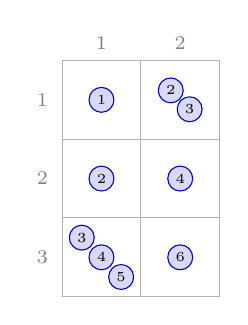
\begin{tikzpicture}[baseline=(current bounding box.center)]
\draw[gray!60] (0,0.00) -- (2.00,0.00);
\draw[gray!60] (0,-1.00) -- (2.00,-1.00);
\draw[gray!60] (0,-2.00) -- (2.00,-2.00);
\draw[gray!60] (0,-3.00) -- (2.00,-3.00);
\draw[gray!60] (0.00,0) -- (0.00,-3.00);
\draw[gray!60] (1.00,0) -- (1.00,-3.00);
\draw[gray!60] (2.00,0) -- (2.00,-3.00);
\node[font=\scriptsize,gray] at (-0.25,-0.50) {1};
\node[font=\scriptsize,gray] at (-0.25,-1.50) {2};
\node[font=\scriptsize,gray] at (-0.25,-2.50) {3};
\node[font=\scriptsize,gray] at (0.50,0.22) {1};
\node[font=\scriptsize,gray] at (1.50,0.22) {2};
\node[circle,draw=cA,fill=cA!15,inner sep=0pt,minimum size=9pt,font=\tiny] at (0.50,-0.50) {1};
\node[circle,draw=cA,fill=cA!15,inner sep=0pt,minimum size=9pt,font=\tiny] at (1.38,-0.38) {2};
\node[circle,draw=cA,fill=cA!15,inner sep=0pt,minimum size=9pt,font=\tiny] at (1.62,-0.62) {3};
\node[circle,draw=cA,fill=cA!15,inner sep=0pt,minimum size=9pt,font=\tiny] at (0.50,-1.50) {2};
\node[circle,draw=cA,fill=cA!15,inner sep=0pt,minimum size=9pt,font=\tiny] at (1.50,-1.50) {4};
\node[circle,draw=cA,fill=cA!15,inner sep=0pt,minimum size=9pt,font=\tiny] at (0.25,-2.25) {3};
\node[circle,draw=cA,fill=cA!15,inner sep=0pt,minimum size=9pt,font=\tiny] at (0.50,-2.50) {4};
\node[circle,draw=cA,fill=cA!15,inner sep=0pt,minimum size=9pt,font=\tiny] at (0.75,-2.75) {5};
\node[circle,draw=cA,fill=cA!15,inner sep=0pt,minimum size=9pt,font=\tiny] at (1.50,-2.50) {6};\end{tikzpicture}\ \ {\small\begin{tabular}{@{}l@{}}$P$ 第 1 列：$1,1,1,1,1,2$\\$Q$ 第 1 列：$1,1,1,2,3,3$\end{tabular}}\qquad $A^\flat$:\ 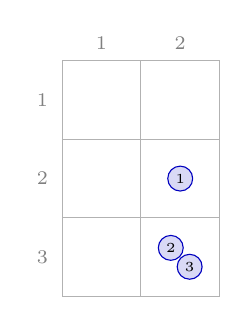
\begin{tikzpicture}[baseline=(current bounding box.center)]
\draw[gray!60] (0,0.00) -- (2.00,0.00);
\draw[gray!60] (0,-1.00) -- (2.00,-1.00);
\draw[gray!60] (0,-2.00) -- (2.00,-2.00);
\draw[gray!60] (0,-3.00) -- (2.00,-3.00);
\draw[gray!60] (0.00,0) -- (0.00,-3.00);
\draw[gray!60] (1.00,0) -- (1.00,-3.00);
\draw[gray!60] (2.00,0) -- (2.00,-3.00);
\node[font=\scriptsize,gray] at (-0.25,-0.50) {1};
\node[font=\scriptsize,gray] at (-0.25,-1.50) {2};
\node[font=\scriptsize,gray] at (-0.25,-2.50) {3};
\node[font=\scriptsize,gray] at (0.50,0.22) {1};
\node[font=\scriptsize,gray] at (1.50,0.22) {2};
\node[circle,draw=cA,fill=cA!15,inner sep=0pt,minimum size=9pt,font=\tiny] at (1.50,-1.50) {1};
\node[circle,draw=cA,fill=cA!15,inner sep=0pt,minimum size=9pt,font=\tiny] at (1.38,-2.38) {2};
\node[circle,draw=cA,fill=cA!15,inner sep=0pt,minimum size=9pt,font=\tiny] at (1.62,-2.62) {3};\end{tikzpicture}\ \ {\small\begin{tabular}{@{}l@{}}$P$ 第 2 列：$2,2,2$\\$Q$ 第 2 列：$2,3,3$\end{tabular}}}

\newcommand{\FulHook}{%
$h(i,j)=\begin{ytableau}9 & 8 & 7 & 5 & 4 & 1 \\ 7 & 6 & 5 & 3 & 2 \\ 6 & 5 & 4 & 2 & 1 \\ 3 & 2 & 1\end{ytableau}\qquad 5+j-i=\begin{ytableau}*(cB!35) 5 & 6 & 7 & 8 & 9 & 10 \\ 4 & *(cB!35) 5 & 6 & 7 & 8 \\ 3 & 4 & *(cB!35) 5 & 6 & 7 \\ 2 & 3 & 4\end{ytableau}$}


% ---------------------------------------------------------------------
\section{第 1 章回顧：列插入、表的字與滑動（動畫 F01--F08）}\label{sec:f-recap}

這一節只把後面各章要用的定義集中寫一次（動畫 F01--F08 有完整的示範）。

\textbf{Young 圖與表。}分割 $\lambda=(\lambda_1\ge\lambda_2\ge\cdots)$ 畫成 Young 圖：第 $i$ 列有 $\lambda_i$ 格、靠左對齊、第一列在最上面。
在格子裡填正整數，每一列由左到右\textbf{弱遞增}、每一行由上到下\textbf{嚴格遞增}，就是一個（半標準）\textbf{表}；
$1,\ldots,n$ 各用一次的叫\textbf{標準表}。從 $\lambda$ 挖掉左上角的小圖 $\mu$ 得到斜形狀 $\lambda/\mu$，填法相同的叫\textbf{斜表}。

\textbf{列插入 $T\leftarrow x$} \fulref{p.7}。把 $x$ 放進第一列：如果這一列沒有比 $x$ 大的數，$x$ 接在列尾；
否則 $x$ 擠出「最左邊、比 $x$ 大」的那個數，被擠出的數再用同樣的規則插入下一列，直到某個數接在列尾（可能自成新的一列）。
結果仍是表，形狀多出一個外角。知道新格子在哪裡，就能反向擠出，還原 $T$ 與 $x$。

\textbf{表的字與乘積} \fulref{p.11}。表的\textbf{字} $w(T)$：從最下面一列讀到最上面一列，每列由左往右。
乘積 $T\cdot U$：把 $w(U)$ 的字母依序列插入 $T$。

\begin{figure}[H]
\centering
\FulRecap
\caption{列插入 $T\leftarrow 2$：2 擠出 3、3 擠出 5、5 擠出 6、6 接在第 4 列尾（\colorbox{yellow!45}{黃色}是擠壓路徑，
\colorbox{cC!35}{綠色}是新格子 $(4,3)$）。右邊是乘積 $T\cdot U$：把 $w(U)=2\,1\,3$ 依序插入 $T$。
這裡 $w(T)=5\,6\,4\,4\,6\,2\,3\,5\,5\,1\,2\,2\,3$。}
\label{fig:f-recap}
\end{figure}

\textbf{滑動與 rectification} \fulref{p.12--13}。在斜表裡挑一個\textbf{內角}（$\mu$ 的角）當洞，
把洞右邊與下面兩個數中\textbf{較小}的滑進洞（相等時取下面的），洞跟著移動，直到洞成為外角、被拿掉。
一直滑到沒有內角，得到一個表，叫做 $S$ 的 \textbf{rectification} $\mathrm{Rect}(S)$。
把 $T$ 放在左下、$U$ 放在右上、中間補一塊空白矩形，得到斜表 $T*U$。

\begin{keybox}[第 1 章留下的三個 Claim（第 2--3 章證明它們）]
\begin{enumerate}[nosep]
\item 乘積有結合律：$(T\cdot U)\cdot V=T\cdot(U\cdot V)$。
\item $\mathrm{Rect}(S)$ 與內角的挑法無關。
\item $\mathrm{Rect}(T*U)=T\cdot U$。
\end{enumerate}
三者都由第 2 章的主定理（\S\ref{sec:f-slides}）推出，主定理的唯一性在第 3 章（\S\ref{sec:f-unique}）證明。
\end{keybox}

% ---------------------------------------------------------------------
\section{第 2 章：字與 plactic monoid（動畫 F09--F13）}\label{sec:f-ch2}

\subsection{字與 Knuth 變換}\label{sec:f-knuth}

\textbf{由字還原表} \fulref{p.17}。把字在每個「下一個字母比前一個小」的地方切開，切出的弱遞增片段由下往上疊起來，
就是原來的表。例如 $5\,6\,4\,4\,6\,2\,3\,5\,5\,1\,2\,2\,3$ 切成 $56\mid 446\mid 2355\mid 1223$，正是圖~\ref{fig:f-recap} 中 $T$ 的四列。
不是每個字都來自表：$3\,4\,1\,4$ 切成 $34\mid 14$，疊起來第 2 行是 4 在 4 上面，不是嚴格遞增。
但\textbf{每個字都是某個斜表的字}：每段當一列，每一列放在下一列的整個右上方，各行至多一格，條件自動成立（圖~\ref{fig:f-runs}）。

\begin{figure}[H]
\centering
\FulRuns
\caption{字 $w=1\,3\,4\,2\,3\,4\,1\,2\,2\,3\,3\,2$ 切成 $134\mid 234\mid 12233\mid 2$，排成階梯形的斜表，它的字就是 $w$。}
\label{fig:f-runs}
\end{figure}

\textbf{用字的語言寫列插入} \fulref{p.18}。把一列的字寫成 $u\,x'\,v$：$x'$ 是第一個比 $x$ 大的字母，
所以 $u\le x<x'\le v$（意思是 $u$ 的每個字母 $\le x$、$v$ 的每個字母 $\ge x'$）。插入 $x$ 就是
\[
(u\,x'\,v)\cdot x\ \longmapsto\ x'\cdot(u\,x\,v),
\]
被擠出的 $x'$ 移到這一列的左邊，而在字裡，下一列恰好就在左邊。圖~\ref{fig:f-recap} 的插入寫成四行：
\[
\begin{aligned}
(56)(446)(2355)(1223)\cdot 2&\mapsto(56)(446)(2355)\cdot 3\cdot(1222)\mapsto(56)(446)\cdot 5\cdot(2335)(1222)\\
&\mapsto(56)\cdot 6\cdot(445)(2335)(1222)=(566)(445)(2335)(1222).
\end{aligned}
\]

\textbf{Knuth 的拆解} \fulref{p.18--19}。每一行還可以再拆成更小的步：先讓 $x$ 一格一格往左移過 $v$ 的字母，
再讓 $x'$ 一格一格往左移過 $u$ 的字母。每一步只動三個相鄰的字母、交換其中兩個，而且只有兩種：
\begin{figure}[H]
\centering
\FulKnuthRules
\caption{兩種基本變換與記法：$K'$ 是把 $x$ 插入一列 $[\,y\ z\,]$（$x$ 擠出 $y$），$K''$ 是把 $y$ 插入 $[\,x\ z\,]$（$y$ 擠出 $z$）。
插入前後的字分別是左邊與右邊的三個字母。}
\label{fig:f-knuth-rules}
\end{figure}
換句話說：一個字母 $y$ 同一側的兩個鄰居若一個比 $y$ 小、一個比 $y$ 大，就可以交換它們
（有相等時，照「相等的字母左邊的算小」來判斷）。

\begin{keybox}[Knuth 等價]
對字裡三個相鄰的字母做一次 $K'$、$K''$ 或它們的反方向，叫做一次\textbf{基本 Knuth 變換}。
兩個字若能用一串基本變換互相變到，就說它們 \textbf{Knuth 等價}，記作 $w\equiv w'$。
\end{keybox}

\begin{thmbox}[命題 1 \fulref{p.19}]
對任何表 $T$ 與正整數 $x$，$w(T\leftarrow x)\equiv w(T)\cdot x$。所以 $w(T\cdot U)\equiv w(T)\cdot w(U)$。
\end{thmbox}

表~\ref{tab:f-chain} 是圖~\ref{fig:f-recap} 的插入拆成的 8 步。第 1 列 $1\,2\,2\,3$：$x=2$ 擠出 $x'=3$，$v$ 是空的，
$3$ 往左移過 $u=1\,2\,2$，三步 $K''$；第 2 列：$3$ 擠出 $5$，先用一步 $K'$ 越過 $v=5$，再用兩步 $K''$ 越過 $u=2\,3$；
第 3 列：$5$ 擠出 $6$，兩步 $K''$ 越過 $4\,4$；第 4 列：$6$ 接在 $5\,6$ 後面，字已經是 $w(T\leftarrow 2)$。

\begin{table}[H]
\centering
\FulChain
\caption{$w(T)\cdot 2\equiv w(T\leftarrow 2)$ 的 8 步基本變換（每一步動到的三個字母標成橘色）。}
\label{tab:f-chain}
\end{table}

\begin{notebox}
一個等價類有多少個字？若 $T$ 的形狀是 $\lambda$，與 $w(T)$ 等價的字恰有 $f^\lambda$ 個（$f^\lambda$ = 形狀 $\lambda$ 的標準表個數，
書 p.57 練習 16，理由見 \S\ref{sec:f-rs}）。例如 $1\,3\,2\equiv 3\,1\,2$，而 $f^{(2,1)}=2$。
\end{notebox}

% ---------------------------------------------------------------------
\subsection{滑動、主定理與 plactic monoid}\label{sec:f-slides}

滑動的中途會出現「有洞」的表；它的字照常讀，跳過洞。\textbf{水平滑動}（洞右邊的數往左移）字完全不變；
\textbf{垂直滑動}（洞下面的數往上移）字會變，但仍然 Knuth 等價。最簡單的情形 \fulref{p.20}：上列 $u\ \square\ y$、
下列 $v\ x\ z$，$x$ 往上滑。用 $u,v,x,y,z=1,2,3,4,5$，字從 $v\,x\,z\,u\,y=2\,3\,5\,1\,4$ 變成 $v\,z\,u\,x\,y=2\,5\,1\,3\,4$，
四步基本變換就能接起來（圖~\ref{fig:f-slide}）。一般情形把 $u,v,y,z$ 換成整段的遞增列，對列長用歸納法，每一步用一次命題 1 \fulref{p.21--22}。

\begin{figure}[H]
\centering
\FulSlide
\caption{垂直滑動前後的字 Knuth 等價：$23514\equiv 25134$（每一步動到的三個字母標成橘色）。}
\label{fig:f-slide}
\end{figure}

\begin{thmbox}[命題 2 \fulref{p.22}]
若一個斜表可以經由一串滑動變成另一個，它們的字 Knuth 等價。
\end{thmbox}

\begin{thmbox}[主定理 \fulref{p.22}]
每個字都恰好與\textbf{一個}表的字 Knuth 等價。
\end{thmbox}

\textbf{存在}很容易：把 $w=x_1x_2\cdots x_r$ 的字母依序插入空表，
\[
P(w)=\bigl(\cdots\bigl((x_1\leftarrow x_2)\leftarrow x_3\bigr)\leftarrow\cdots\bigr)\leftarrow x_r ,
\]
由命題 1，每插入一個字母，等價類都不變，所以 $w\equiv w(P(w))$。例如 $w=1\,3\,4\,2\,3\,4\,1\,2\,2\,3\,3\,2$ 的
$P(w)$ 是圖~\ref{fig:f-increasing} 右邊的表，它的字 $3\,4\,4\,2\,3\,3\,1\,1\,2\,2\,2\,3$ 和 $w$ 不同，卻彼此等價。
\textbf{唯一}則需要新的想法，留到第 3 章（\S\ref{sec:f-unique}）。先承認它，就得到：

\begin{thmbox}[推論 \fulref{p.23}]
\begin{enumerate}[nosep]
\item $\mathrm{Rect}(S)$ 是唯一與 $w(S)$ 等價的表；$\mathrm{Rect}(S)=\mathrm{Rect}(S')$ 若且唯若 $w(S)\equiv w(S')$。
\item 乘積 $T\cdot U$ 的三種做法——把 $w(U)$ 插入 $T$、$\mathrm{Rect}(T*U)$、唯一與 $w(T)\,w(U)$ 等價的表——結果相同。
\end{enumerate}
\end{thmbox}

第 1 點由命題 2 得到，所以 $\mathrm{Rect}(S)$ 與挑內角的順序無關（Claim 2）。例如 p.12 的斜表 $S$，
$w(S)=5\,5\,2\,3\,6\,2\,4\,4\,6\,2$，把它插入空表與把 $S$ 滑成表，都得到 $\yts{22246,346,55}$。
第 2 點：三種做法的字都與 $w(T)\,w(U)$ 等價，所以是同一個表（Claim 3）；而字的連接顯然有結合律，所以乘積也有（Claim 1）。
圖~\ref{fig:f-recap} 的例子 $T\cdot U=\yts{11223,2235,345,466,5}$ 三種做法都得到。

\textbf{Plactic monoid} \fulref{p.23--24}。把字依 Knuth 等價分類，等價類的乘法就是把字接起來（等價的字接起來仍等價），
得到一個么半群 $\mathcal{M}$，Lascoux 與 Schützenberger 稱為 plactic monoid。主定理說：$\mathcal{M}$ 和「表＋乘積」是同一個東西。
再取以表為基底的自由 $\mathbb{Z}$-模、以表的乘積為乘法，得到 \textbf{tableau ring} $R_{[m]}$（數字取自 $[m]=\{1,\ldots,m\}$；
有結合律、不交換）。$T\mapsto x^T$（數字 $i$ 出現幾次，$x_i$ 就幾次方）是 $R_{[m]}\to\mathbb{Z}[x_1,\ldots,x_m]$ 的環同態。

% ---------------------------------------------------------------------
\subsection{Pieri 公式}\label{sec:f-pieri}

在 tableau ring 裡，令 $S_\lambda=S_\lambda[m]$ 為所有形狀 $\lambda$、數字在 $[m]$ 的表的和；它的像就是 Schur 多項式 $s_\lambda(x_1,\ldots,x_m)$。

\begin{thmbox}[Pieri 公式 \fulref{p.24}]
\[
\begin{aligned}
S_\lambda\cdot S_{(p)}&=\sum_{\mu} S_\mu &&(\mu/\lambda\ \text{是 $p$ 格的\textbf{水平帶}：任兩格不同行}),\\
S_\lambda\cdot S_{(1^p)}&=\sum_{\mu} S_\mu &&(\mu/\lambda\ \text{是 $p$ 格的\textbf{垂直帶}：任兩格不同列}).
\end{aligned}
\]
\end{thmbox}

理由是第 1 章 \S1.1 的命題（動畫 F05）：依序插入一列（弱遞增的數），新格子一格比一格靠右、而且不會往下，所以新長出的格子是水平帶；
反過來，若 $U$ 的形狀 $\mu$ 比 $\lambda$ 多一條 $p$ 格的水平帶，從最右邊的新格子開始反向擠出 $p$ 次，
就把 $U$ \textbf{唯一地}拆成 $T\cdot V$（$T$ 的形狀 $\lambda$、$V$ 是一列）。插入一行（嚴格遞增的數）的情形同理，得到垂直帶。

\begin{figure}[H]
\centering
\FulPieri
\caption{$\lambda=(2,1)$、$p=2$。加\textcolor{cLeft}{水平帶}得到 $(4,1)$、$(3,2)$、$(3,1,1)$、$(2,2,1)$；
加\textcolor{cRight}{垂直帶}得到 $(3,2)$、$(3,1,1)$、$(2,2,1)$、$(2,1,1,1)$。}
\label{fig:f-pieri}
\end{figure}

數一數 $m=3$ 的情形：形狀 $(2,1)$ 的表有 8 個、長 2 的列有 6 個，$8\cdot 6=48=24+15+6+3$，右邊正是四種 $\mu$ 的表數。
把每個表換成 $x^T$，一列的表的和是完全對稱多項式 $h_p$、一行的表的和是基本對稱多項式 $e_p$，得到
\[
s_\lambda\,h_p=\sum s_\mu\ (\text{水平帶}),\qquad s_\lambda\,e_p=\sum s_\mu\ (\text{垂直帶}).
\]
用三個變數比較 $x_1^2x_2^2x_3$ 的係數：$s_{(2,1)}h_2$ 那邊是 $6=2+2+1+1$，$s_{(2,1)}e_2$ 那邊是 $4=2+1+1+0$
（最後一項是 0：$s_{(2,1,1,1)}$ 要 4 個不同的數，三個變數不夠）。

% ---------------------------------------------------------------------
\subsection{Kostka 數與兩種序}\label{sec:f-kostka}

表的\textbf{內容}是 $\mu=(\mu_1,\mu_2,\ldots)$：數字 $i$ 出現 $\mu_i$ 次。\textbf{Kostka 數} $K_{\lambda\mu}$ = 形狀 $\lambda$、內容 $\mu$ 的表的個數 \fulref{p.25}。
等價的說法：把數字 $\le k$ 的格子取出來，得到形狀 $\lambda^{(k)}$，於是 $\varnothing\subset\lambda^{(1)}\subset\cdots\subset\lambda$，每一步多一條 $\mu_k$ 格的水平帶；
$K_{\lambda\mu}$ 就是這種鏈的個數。

\begin{figure}[H]
\centering
\FulKostkaTabs
\caption{$\lambda=(3,2)$、$\mu=(2,2,1)$ 的兩個表（\textcolor{cLeft}{1}、\textcolor{cB}{2}、\textcolor{cRight}{3} 分色）與它們的水平帶鏈，所以 $K_{(3,2),(2,2,1)}=2$。}
\label{fig:f-kostka-tabs}
\end{figure}

反覆使用 Pieri 公式 $s_\lambda h_p=\sum s_\mu$，從 1 開始依序乘上 $h_{\mu_1},h_{\mu_2},\ldots$，每乘一次就加一條水平帶：
\[
h_{\mu_1}h_{\mu_2}\cdots h_{\mu_\ell}=\sum_\lambda K_{\lambda\mu}\,s_\lambda ,\qquad\text{例如}\quad h_2h_1h_1=s_{(4)}+2s_{(3,1)}+s_{(2,2)}+s_{(2,1,1)} .
\]
同理 $e_{\mu_1}\cdots e_{\mu_\ell}=\sum_\lambda K_{\tilde\lambda\mu}\,s_\lambda$（$\tilde\lambda$ 是共軛分割；垂直帶轉置後就是水平帶）。

\textbf{兩種序} \fulref{p.26}。\textbf{字典序}：從第一項比起，第一個不同的地方較大者為大，這是全序。
\textbf{支配序} $\mu\trianglelefteq\lambda$：每個 $i$ 都有 $\mu_1+\cdots+\mu_i\le\lambda_1+\cdots+\lambda_i$。
包含 $\Rightarrow$ 支配 $\Rightarrow$ 字典序，反過來都不對：$(2,2)\trianglelefteq(3,1)$ 但 $(2,2)\not\subset(3,1)$；
$(4,1,1)$ 的字典序比 $(3,3)$ 大，卻不支配它（$4+1<3+3$）；$(2,2,2)$ 與 $(3,1,1,1)$ 在支配序下不可比。

由定義，$K_{\lambda\lambda}=1$，而 $\mu$ 的字典序比 $\lambda$ 大時 $K_{\lambda\mu}=0$（第一列放不下那麼多 1，依此類推）。
所以把分割依字典序由小到大排，Kostka 矩陣是對角線全為 1 的下三角矩陣（表~\ref{tab:f-kostka}）。
更精確地（練習 2）：$K_{\lambda\mu}\ne 0$ 若且唯若 $\mu\trianglelefteq\lambda$；字典序較大還不夠，例如 $K_{(4,1,1),(3,3)}=0$。

\begin{table}[H]
\centering
\FulKostkaMatrix
\caption{$n=4$ 的 Kostka 矩陣 $K_{\lambda\mu}$（列 $\lambda$、行 $\mu$，字典序由小到大）：下三角、對角線為 1。}
\label{tab:f-kostka}
\end{table}

下三角矩陣可以反解，所以 $s_\lambda$ 能寫成 $h_\mu$ 的整係數組合，而 $h_\mu$ 是對稱多項式——\textbf{Schur 多項式是對稱的}。
這也推出 $K_{\lambda\mu}$ 與 $\mu$ 各項的順序無關（例如 $K_{(3,2),(2,2,1)}=K_{(3,2),(1,2,2)}=K_{(3,2),(2,1,2)}=2$），第 4 章會直接證明（\S\ref{sec:f-apps}）。

% ---------------------------------------------------------------------
\subsection{行字}\label{sec:f-colword}

另一種把表攤平的方法 \fulref{p.27}：由左到右逐行，每一行\textbf{由下往上}讀，得到\textbf{行字} $w_{\mathrm{col}}(T)$。
圖~\ref{fig:f-recap} 的 $T$：$w_{\mathrm{col}}(T)=5421\ 6432\ 652\ 53$，而 $w_{\mathrm{row}}(T)=56\ 446\ 2355\ 1223$。兩個字長得不一樣，但

\begin{thmbox}[(10) \fulref{p.27}]
$w_{\mathrm{col}}(T)\equiv w_{\mathrm{row}}(T)$。（把行字插入空表，長出來的正是 $T$。）
\end{thmbox}

這由一個更一般的事實得到。\textbf{Lemma 1}：斜表被一條水平或垂直的線切成 $T'$、$T''$，則 $w(T)\equiv w(T')\cdot w(T'')$。
水平切是字的定義本身。垂直切：把左塊 $T'$ 往下移到右塊 $T''$ 的左下，得到斜表 $T'*T''$，它的字正是 $w(T')\,w(T'')$；
再從 $T'$ 正上方的內角由右到左一格一格滑回去，就回到 $T$，由命題 2 得證（圖~\ref{fig:f-cut}）。
一次切下最左邊的一行，對剩下的再切，得到 $w(T)\equiv w(C_1)\,w(C_2)\cdots$，而單獨一行的字就是由下往上讀，所以就是 (10)。

\begin{figure}[H]
\centering
\FulCut
\caption{在第 2 行之後垂直切開：$T'$（左兩行）與 $T''$；$T'*T''$ 的字是 $56442312\cdot 65523$，滑回去仍是 $T$。}
\label{fig:f-cut}
\end{figure}

\begin{notebox}
還有更強的 Lemma 2 \fulref{p.28}：$w_{\mathrm{col}}(T)$ 與 $w_{\mathrm{row}}(T)$ 只用 $K'$ 一種變換（及其反方向）就能互變。書到附錄 A 才用到。
\end{notebox}

% Young 表講義第 2 段：第 3–4 章（動畫 F14–F19）
% 圖與表在 fulton/figs.tex（由 fulton/make_figs.py 產生，part1.tex 已 \input）。

% ---------------------------------------------------------------------
\section{第 3 章：遞增子序列與主定理的證明（動畫 F14--F15）}\label{sec:f-ch3}

\subsection{遞增子序列與 $L(w,k)$}\label{sec:f-increasing}

Schensted 發明列插入，原本是為了研究字裡的遞增子序列 \fulref{p.30}。令 $L(w,k)$ 為從 $w$ 取出 $k$ 個\textbf{互不相交}的
弱遞增子序列，長度總和的最大值。例子 $w=1\,3\,4\,2\,3\,4\,1\,2\,2\,3\,3\,2$：$L(w,1)=6$、$L(w,2)=9$、$k\ge 3$ 時 $L(w,k)=12$（圖~\ref{fig:f-increasing}）。

\begin{figure}[H]
\centering
\FulIncreasing
\caption{$w$ 的 1、2、3 個不相交弱遞增子序列（分色）達到 $L(w,k)=6,9,12$；右邊是 $P(w)$，它的各列長 $6,3,3$。}
\label{fig:f-increasing}
\end{figure}

長度的分配並不唯一：$L(w,2)=9$ 可以是 $6+3$，也可以是 $5+4$；而且\textbf{沒有}長度 $6,3,3$ 的三條（程式窮舉確認），
也就是 $k=1$ 時最長的那一條，不一定能保留到 $k=3$。可是換成與 $w$ 等價的 $w'=w(P(w))=3\,4\,4\,2\,3\,3\,1\,1\,2\,2\,2\,3$，
從右邊一塊一塊取（也就是 $P(w)$ 的各列），立刻得到最好的取法 $6$、$6+3$、$6+3+3$。這兩件事一般都成立：

\begin{thmbox}[Lemma 1 \fulref{p.32}]
若 $w$ 是形狀 $\lambda$ 的表的字，則 $L(w,k)=\lambda_1+\cdots+\lambda_k$。
\end{thmbox}

理由：在表的字裡，一條遞增子序列在圖上一定由左往右、從不往下走（同一行下面的數較大，卻在字裡排在前面），
所以每一行至多用到一格。$k$ 條加起來不會超過前 $k$ 列的格數，而前 $k$ 列本身就達到這個數。

\begin{thmbox}[Lemma 2 \fulref{p.32--33}]
若 $w\equiv w'$，則對所有 $k$，$L(w,k)=L(w',k)$。
\end{thmbox}

只需看一次基本變換，例如 $K'$：$w=u\,y\,x\,z\,v$、$w'=u\,y\,z\,x\,v$（$x<y\le z$）。$w'$ 的遞增子序列不會同時含 $z$ 和 $x$（$z>x$ 卻在前面），
所以照搬到 $w$ 仍遞增，$L(w,k)\ge L(w',k)$。反方向的關鍵情形是：$w$ 的某一條同時用到 $x$、$z$（形如 $u_1\,x\,z\,v_1$），
另一條用到 $y$（形如 $u_2\,y\,v_2$）。這時把兩條換成 $u_2\,y\,z\,v_1$ 與 $u_1\,x\,v_2$——\textbf{交換尾巴}，兩條在 $w'$ 裡都遞增，總長不變。
$K''$ 的情形相同。

由兩個 Lemma，與 $w$ 等價的任何表，形狀都由 $w$ 決定：$\lambda_k=L(w,k)-L(w,k-1)$。

% ---------------------------------------------------------------------
\subsection{唯一性的證明}\label{sec:f-unique}

\begin{thmbox}[Lemma 3 \fulref{p.33}]
若 $w\equiv w'$，各自去掉 $p$ 個最大的字母（一樣大時右邊的算比較大，先去掉）與 $q$ 個最小的字母，剩下的字仍然等價。
\end{thmbox}

一樣只看一次基本變換：去掉的若不是被交換的那三個字母，顯然；若是，去掉最大字母時只可能去掉 $z$，兩邊剩下的字完全相同。
例：$1\,3\,4\,2\,3\,1\,3$ 去掉 3 個最大的（4 與右邊兩個 3）剩下 $1\,3\,2\,1$。

\textbf{主定理唯一性的證明} \fulref{p.34}。設 $w\equiv w(T)$。形狀已由 $L(w,k)$ 決定。令 $x$ 為 $w$ 最大的字母，
$w_0$ 為去掉最右邊那個 $x$ 的字，$T_0$ 為從 $T$ 去掉最右邊的 $x$ 的表；由 Lemma 3，$w_0\equiv w(T_0)$，
由歸納法 $T_0$ 是唯一的。$T$ 比 $T_0$ 多一格，$x$ 只能放在那一格，所以 $T$ 也是唯一的。

這個證明本身就是一個演算法：只用 $L(w,k)$，一次去掉一個最大字母，看形狀少了哪一格，那個字母就放那一格（表~\ref{tab:f-rebuild}）。
（實際計算當然還是用列插入比較快。）

\begin{table}[H]
\centering
\FulRebuild
\caption{由 $L(w,k)$ 重建 $P(w)$：第 $p$ 列是去掉 $p$ 個最大字母後的字 $w_p$；它的形狀比 $w_{p+1}$ 多出的那一格，就是 $w_p$ 最大字母的位置。
由下往上填回去，得到圖~\ref{fig:f-increasing} 右邊的 $P(w)$。}
\label{tab:f-rebuild}
\end{table}

\begin{keybox}[到這裡]
主定理成立：每個字恰與一個表的字等價。於是第 2 章的推論、以及第 1 章的三個 Claim（\S\ref{sec:f-recap}）全部證完。
\end{keybox}

\textbf{嚴格遞減子序列} \fulref{p.34，練習 1--2}。同樣的論證給出：最長嚴格遞減子序列的長度 = $P(w)$ 的列數；
$k$ 條不相交嚴格遞減子序列的最大總長 = 前 $k$ 行的格數。推論（Erdős–Szekeres）：長度大於 $n^2$ 的字，一定有長度大於 $n$ 的
遞增或嚴格遞減子序列——$P(w)$ 的格子比 $n\times n$ 多，第一列或列數總有一個超過 $n$。
例：$w=4\,9\,2\,10\,6\,1\,8\,3\,7\,5$（長度 $10>3^2$），$P(w)=\yts{135,267,48{10},9}$，
形狀 $(3,3,3,1)$：最長遞增 3、最長嚴格遞減 4。

\begin{notebox}
這些是 Greene 定理（1976）的特例：任何有限偏序集都可定義 $L(W,k)$，其差分與「反鏈」的差分恰好是一對共軛分割 \fulref{p.35}。本書不需要。
\end{notebox}

% ---------------------------------------------------------------------
\section{第 4 章：Robinson–Schensted–Knuth 對應（動畫 F16--F19）}\label{sec:f-ch4}

\subsection{Robinson–Schensted 對應}\label{sec:f-rs}

建 $P(w)$ 的同時，在第 $k$ 步長出的新格子寫上 $k$，得到同形狀的\textbf{記錄表} $Q(w)$ \fulref{p.36--37}；
新格子總是外角，所以 $Q(w)$ 是標準表。例 $w=5\,4\,8\,2\,3\,4\,1\,7\,5\,3\,1$（圖~\ref{fig:f-rs}）。

\begin{figure}[H]
\centering
\FulRS
\caption{$w=5\,4\,8\,2\,3\,4\,1\,7\,5\,3\,1$：前 4 步的 $(P_k,Q_k)$，以及最後的 $(P,Q)$。}
\label{fig:f-rs}
\end{figure}

\textbf{反過來。}找出 $Q$ 最大的數 $r$ 所在的格子，從 $P$ 的同一格反向擠出，擠出第一列的數就是 $x_r$；
再把 $r$ 從 $Q$ 拿掉，重複下去，一步一步還原 $w$。所以 $(P,Q)$ 決定 $w$。

\begin{thmbox}[Robinson–Schensted 對應 \fulref{p.38}]
長度 $r$、字母取自 $[n]$ 的字 $\longleftrightarrow$ 同形狀的一對 $(P,Q)$：$P$ 是數字在 $[n]$ 的表，$Q$ 是 $r$ 格的標準表。
特別地，$S_n$ 的排列 $\longleftrightarrow$ 同形狀的一對標準表（Robinson 對應）。
\end{thmbox}

數一數排列，得到 $n!=\sum_{\lambda\vdash n}(f^\lambda)^2$：$3!=1+4+1$、$4!=1+9+4+9+1=24$。
這也說明 \S\ref{sec:f-knuth} 的小註：$P$ 固定、$Q$ 跑遍 $f^\lambda$ 個標準表，就是與 $w(P)$ 等價的所有字。
另外 $Q$ 決定排列的升降：$w_i>w_{i+1}$ 若且唯若 $i+1$ 在 $Q$ 裡位於 $i$ 的下面一列以下（練習 17）。

% ---------------------------------------------------------------------
\subsection{R-S-K：雙列陣列與對稱定理}\label{sec:f-rsk}

Knuth 的推廣 \fulref{p.38--39}：考慮雙列陣列 $\omega=\left(\begin{smallmatrix}u_1&\cdots&u_r\\ v_1&\cdots&v_r\end{smallmatrix}\right)$，
要求它是\textbf{字典序}：上列 $u_1\le u_2\le\cdots\le u_r$，上列相同的地方下列也弱遞增。把下列 $v_k$ 依序列插入得到 $P$，
同時把上列 $u_k$ 放進新長出的格子得到 $Q$。$Q$ 也是表：上列相同的那幾步，插入的 $v$ 弱遞增，由第 1 章的 Row Bumping Lemma，
新格子一格比一格靠右、不往下，所以相同的 $u$ 不會疊在同一行。

\begin{figure}[H]
\centering
\FulArray
\caption{練習 1 \fulref{p.40}：陣列 $\omega$、它的矩陣 $A$（$a(i,j)$ = 欄 $\binom{i}{j}$ 出現的次數），與對應的 $(P,Q)$。}
\label{fig:f-array}
\end{figure}

\begin{thmbox}[R-S-K 定理 \fulref{p.40}]
字典序的雙列陣列 $\longleftrightarrow$ 同形狀的一對表 $(P,Q)$，而且
(i) $P$ 的數就是下列、$Q$ 的數就是上列；(ii) $\omega$ 是字（上列是 $1,\ldots,r$）$\iff$ $Q$ 是標準表；
(iii) $\omega$ 是排列 $\iff$ $P$、$Q$ 都是標準表。
\end{thmbox}

\textbf{矩陣的語言} \fulref{p.41}。陣列可以記成矩陣 $A$：第 $i$ 列和 = $Q$ 裡 $i$ 的個數，第 $j$ 行和 = $P$ 裡 $j$ 的個數。
圖~\ref{fig:f-array} 的 $A$ 列和是 $(3,2,4)$、行和是 $(5,4)$，正好是 $Q$ 與 $P$ 的內容。所以 R-S-K 是「非負整數矩陣 $\leftrightarrow$ 同形狀的表對」。

\begin{thmbox}[對稱定理（Schützenberger、Knuth）\fulref{p.40}]
若 $\omega$ 對應 $(P,Q)$，則上下翻轉的陣列（即轉置矩陣 $A^{T}$，再排回字典序）對應 $(Q,P)$。
\end{thmbox}

例：$A^T$ 對應的正是 $(Q,P)$（練習 2）。對排列而言，上下翻轉就是取反函數：$P(w^{-1})=Q(w)$、$Q(w^{-1})=P(w)$。
例 $w=3\,1\,4\,2$、$w^{-1}=2\,4\,1\,3$：$P(w)=\yts{12,34}=Q(w^{-1})$，$Q(w)=\yts{13,24}=P(w^{-1})$。
因此對稱矩陣 $\leftrightarrow$ $P=Q$ 的表對，也就是 $\leftrightarrow$ 一個表；對合（$w=w^{-1}$）$\leftrightarrow$ 標準表：
$S_4$ 有 10 個對合 $=1+3+2+3+1=\sum_{\lambda\vdash 4}f^\lambda$。

% ---------------------------------------------------------------------
\subsection{矩陣球構造}\label{sec:f-balls}

不用一次一次地插入，直接從矩陣讀出 $(P,Q)$ 的方法 \fulref{p.42--44}。在 $(i,j)$ 位置放 $a(i,j)$ 個球，同一格的球由西北往東南斜排。
\textbf{編號}：每個球的號碼 = 比它西北方（列號 $\le$、行號 $\le$ 的其他格，以及同一格裡排在前面的）所有球的號碼都大的最小整數。
於是 \textbf{$P$ 的第一列} = 每個號碼最左邊出現的行號，\textbf{$Q$ 的第一列} = 每個號碼最上面出現的列號。

\textbf{導出矩陣 $A^\flat$}：號碼相同的 $\ell$ 個球一定由西南到東北排成一串；除了最後一個，在每個球的右邊、下一個球的正下方放一個新球，
共 $\ell-1$ 個。對 $A^\flat$ 重新編號，讀出 $P$、$Q$ 的第二列；如此重複，直到沒有兩個球同號為止。

\begin{figure}[H]
\centering
\FulBalls
\caption{$A$ 的球與編號，讀出第一列；號碼 2 的兩球（$(1,2)$、$(2,1)$）在 $(2,2)$ 產生新球，號碼 3、4 各在 $(3,2)$ 產生新球，
得到 $A^\flat$，讀出第二列。結果與圖~\ref{fig:f-array} 的 $(P,Q)$ 相同。}
\label{fig:f-balls}
\end{figure}

書上用球的總數做歸納，證明矩陣球構造給出的正是 R-S-K 的 $(P,Q)$（命題 1，p.44--46）。編號的規則對列與行完全對稱，
把 $A$ 轉置，「最左的行」與「最上的列」互換，就得到 $(Q,P)$——\textbf{對稱定理一目了然}。$A$ 是排列矩陣時，這就是 Viennot 的「影子線」構造。

\textbf{對稱矩陣} \fulref{p.47，練習 4}。$A$ 對稱時 $P=Q$，且 $P$ 第一列的長度 $=\operatorname{tr}A+\operatorname{tr}A^\flat$；
由此 $\operatorname{tr}A$ = 形狀中長度為奇數的行數。例 $S=\left(\begin{smallmatrix}2&1\\1&1\end{smallmatrix}\right)$：
$P=Q=\yts{1112,2}$，$\operatorname{tr}S+\operatorname{tr}S^\flat=3+1=4$，各行長 $2,1,1,1$ 中有 3 個奇數 $=\operatorname{tr}S$。
對合的情形：不動點的個數 = 奇數長的行數。

% ---------------------------------------------------------------------
\subsection{R-S-K 的應用}\label{sec:f-apps}

\textbf{Kostka 數與 $\mu$ 的順序無關} \fulref{p.50--51}。先看只有兩個數字的情形：形狀 $(r+s+t,\,r)$、只含 1 與 2 的表，
第 2 列一定全是 2，它上面的 $r$ 格全是 1，第 1 列剩下的是 $s$ 個 1 接 $t$ 個 2；把 $s,t$ 對調，就是內容 $(r+s,r+t)$ 與 $(r+t,r+s)$
的表之間的一一對應（例 $r,s,t=2,3,1$：形狀 $(6,2)$、內容 $(5,3)$ 與 $(3,5)$ 各恰有 1 個表）。一般情形只需交換相鄰的 $\mu_k,\mu_{k+1}$：
在 R-S-K 下，固定 $P$、看 $Q$ 的內容就是看 $A$ 的列和；把 $A$ 切成前 $k-1$ 列 $B$、第 $k,k+1$ 列 $C$、其餘 $D$，則 $P(A)=P(B)\cdot P(C)\cdot P(D)$，
用兩個數字的情形把 $C$ 換成列和對調、$P$ 不變的 $C'$ 即可。於是 \textbf{Schur 多項式是對稱的}（第 2 章借用的事實在此得證）。

\textbf{Cauchy–Littlewood 公式} \fulref{p.52}：
\[
\prod_{i,j}\frac{1}{1-x_i y_j}=\sum_\lambda s_\lambda(x_1,\ldots,x_n)\,s_\lambda(y_1,\ldots,y_m).
\]
左邊展開，是所有非負整數矩陣 $A$ 的 $\prod(x_jy_i)^{a(i,j)}$；若 $A\leftrightarrow(P,Q)$，這一項正是 $x^Py^Q$，而右邊是所有同形狀 $(P,Q)$ 的 $x^Py^Q$ 之和。
小驗算：$2\times2$、元素和為 3 的矩陣有 $\binom{6}{3}=20$ 個 $=\sum_{\lambda\vdash3}d_\lambda(2)^2=16+4+0$
（$d_\lambda(m)$ = 數字取自 $[m]$ 的 $\lambda$ 形表的個數）。

\textbf{計數恆等式} \fulref{p.52}。由 Robinson 與 Robinson–Schensted 對應、對稱定理：
\[
n!=\sum_{\lambda\vdash n}(f^\lambda)^2,\qquad m^n=\sum_{\lambda\vdash n}d_\lambda(m)\,f^\lambda,\qquad
\sum_{\lambda\vdash n}f^\lambda=\#\{w\in S_n:w=w^{-1}\}.
\]
例：$2^3=8=4\cdot1+2\cdot2+0\cdot1$；$n=4$ 的對合有 10 個。

\textbf{兩個鉤長公式} \fulref{p.53--56}。鉤長公式 $f^\lambda=n!/\prod h(i,j)$ 在另一份講義（Chu 論文導讀的附錄 A.13，動畫 M13）已經證明；
書上的例子 $\lambda=(6,5,5,3)$ 得 $f^\lambda=19!/\prod h(i,j)=6{,}651{,}216$。Stanley 的\textbf{鉤–內容公式}：
\[
d_\lambda(m)=\prod_{(i,j)\in\lambda}\frac{m+j-i}{h(i,j)} ,
\]
分子是在對角線上寫 $m$、往右一格加 1、往下一格減 1。$m=5$ 時得 $d_{(6,5,5,3)}(5)=3{,}360$（圖~\ref{fig:f-hook}；書在第 6 章證明，這裡用程式直接列舉驗證）。

\begin{figure}[H]
\centering
\FulHook
\caption{$\lambda=(6,5,5,3)$：左為鉤長 $h(i,j)$，右為 $5+j-i$（\colorbox{cB!35}{對角線}是 $m=5$）。}
\label{fig:f-hook}
\end{figure}

\textbf{遞增與遞減}（練習 12）：最長遞增子序列長 $\ell$、最長遞減子序列長 $k$ 的排列個數 $=\sum(f^\lambda)^2$，
$\lambda$ 跑遍恰有 $k$ 列、$\ell$ 行的形狀。例：$S_4$ 中兩者都是 2 的排列是 $2143,2413,3142,3412$，共 $(f^{(2,2)})^2=4$ 個。

% Young 表講義第 3 段：第 5 章 Littlewood–Richardson 規則（動畫 F20–F24）
% 圖與表在 fulton/figs.tex（由 fulton/make_figs.py 產生，part1.tex 已 \input）。

\section{第 5 章：Littlewood–Richardson 規則（動畫 F20--F24）}\label{sec:f-ch5}

\subsection{表的因數分解與 LR 數}\label{sec:f-factor}

整數可以因數分解：$12=3\times4=2\times6$。表也可以問同樣的問題 \fulref{p.60}：給一個形狀 $\nu$ 的表 $V$，
有幾種寫法 $V=T\cdot U$，其中 $T$ 的形狀是 $\lambda$、$U$ 的形狀是 $\mu$？把這些 $[T,U]$ 的集合記為 $\mathcal T(\lambda,\mu,V)$。
另一個看似無關的集合：形狀 $\nu/\lambda$、rectification 等於給定的 $U_0$（形狀 $\mu$）的斜表，記為 $\mathcal S(\nu/\lambda,U_0)$。

\begin{figure}[H]
\centering
\FulFactor
\caption{$\lambda=\mu=(2,1)$、$\nu=(3,2,1)$。上：$V$ 恰有兩種分解（把 $w(U)=5\,2\,3$ 依序插入 $T$ 就能驗算）。
下：$(3,2,1)/(2,1)$ 上內容 $(2,1)$ 的斜表有 3 個，滑完之後恰好兩個變成 $U_0$。}
\label{fig:f-factor}
\end{figure}

在圖~\ref{fig:f-factor} 的例子裡兩邊都是 2。換一個 $V$（例如 $\yts{112,23,3}$）分解數仍是 2；
其實形狀 $(3,2,1)$ 的 16 個標準表，每一個都恰好有 2 種分解（動畫 F20）。這不是巧合：

\begin{thmbox}[命題 1、2 \fulref{p.58--62}]
(1) 把字典序陣列 $\binom{u_1\cdots u_m}{v_1\cdots v_m}$ 的下列依序插入任何一個表 $T$，並把上列放進新長出的格子，
得到的斜表 $S$ 會 rectify 成 R-S-K 給的那個 $Q$。\\
(2) 由此，$\mathcal T(\lambda,\mu,V_0)$ 與 $\mathcal S(\nu/\lambda,U_0)$ 之間有一一對應（對任何 $V_0$、$U_0$）。
\end{thmbox}

對應的做法：給 $[T,U]$，用 R-S-K 把 $(U,U_0)$ 變成陣列，下列插入 $T$、上列放進新格子，就得到 $\mathcal S$ 裡的斜表；反過來也能還原。
兩個集合彼此不知道對方用的是哪個 $V_0$、$U_0$，所以：

\begin{keybox}[Littlewood–Richardson 數]
$|\mathcal T(\lambda,\mu,V_0)|=|\mathcal S(\nu/\lambda,U_0)|$ 只和形狀 $\lambda,\mu,\nu$ 有關，記作 $c^\nu_{\lambda\mu}$
（推論 1，\fulref{p.62}）。上面的例子 $c^{(3,2,1)}_{(2,1),(2,1)}=2$。
\end{keybox}

\subsection{LR 數的對稱性與乘法公式}\label{sec:f-lrsym}

\begin{thmbox}[推論 2 \fulref{p.62}]
$c^\nu_{\lambda\mu}=c^\nu_{\mu\lambda}=c^{\tilde\nu}_{\tilde\lambda\tilde\mu}$（$\sim$ 是共軛）；而且 $c^\nu_{\lambda\mu}$ 也等於斜表 $\lambda*\mu$ 上
rectify 成某個給定 $\nu$ 形表的斜表個數。
\end{thmbox}

例：$c^{(4,2,1)}_{(2,1),(3,1)}=c^{(4,2,1)}_{(3,1),(2,1)}=c^{(3,2,1,1)}_{(2,1),(2,1,1)}=2$（三個圖一起轉置，數字不變）。
最後一句給了一個判斷 0 的快速方法：滑動時格子只往左上移，外框不會變大，所以 $\nu$ 若放不進 $\lambda*\mu$ 的外框，$c^\nu_{\lambda\mu}=0$。
書上的例子 $\lambda=(2,2)$、$\mu=(3,2)$、$\nu=(3,3,3)$：$|\nu|=4+5$、$\lambda,\mu\subset\nu$ 都沒問題，
但 $\lambda*\mu$ 的第 3 列只有 2 格，$\nu$ 卻要 3 格，所以 $c^{(3,3,3)}_{(2,2),(3,2)}=0$ \fulref{p.63}。

\textbf{乘法公式。}$c^\nu_{\lambda\mu}$ 就是「形狀 $\nu$ 的每個表能寫成 $\lambda$ 形表乘 $\mu$ 形表的方法數」，翻譯到 tableau ring：
\[
S_\lambda\cdot S_\mu=\sum_\nu c^\nu_{\lambda\mu}\,S_\nu ,\qquad S_{\nu/\lambda}=\sum_\mu c^\nu_{\lambda\mu}\,S_\mu
\qquad\text{（推論 3、4，\fulref{p.63}）}，
\]
其中 $S_{\nu/\lambda}$ 是 $\nu/\lambda$ 上所有斜表的 rectification 之和。由 $c^\nu_{\lambda\mu}=c^\nu_{\mu\lambda}$，這些 $S_\lambda$ 生成的子環是交換的；
取像 $T\mapsto x^T$，就得到 Schur 多項式的乘法 $s_\lambda s_\mu=\sum c^\nu_{\lambda\mu}s_\nu$ 與斜 Schur 多項式 $s_{\nu/\lambda}=\sum c^\nu_{\lambda\mu}s_\mu$。

\subsection{反格字與 LR 斜表}\label{sec:f-yamanouchi}

LR 數要怎麼\textbf{算}？關鍵是一種字 \fulref{p.63}。

\begin{keybox}[反格字（Yamanouchi 字）]
從字尾往前讀到任何位置，1 的個數 $\ge$ 2 的個數 $\ge$ 3 的個數 $\ge\cdots$。想成\textbf{倒著開票}：開票過程中，1 號候選人永遠不落後 2 號、
2 號不落後 3 號……。字是反格字的斜表叫做 \textbf{LR 斜表}。
\end{keybox}

例：$2\,1\,3\,2\,1\,2\,1$ 是反格字；$1\,2\,3\,2\,1\,2\,1$ 不是——倒著開到第 6 票（最後 6 個字母 $2\,3\,2\,1\,2\,1$）時，2 號有 3 票、1 號只有 2 票。

\begin{thmbox}[命題 3 \fulref{p.64}]
$c^\nu_{\lambda\mu}$ = 形狀 $\nu/\lambda$、內容 $\mu$ 的 LR 斜表個數。
\end{thmbox}

理由分兩步。\textbf{Lemma 1}：一個斜表是內容 $\mu$ 的 LR 斜表，若且唯若它 rectify 成 $U(\mu)$（第 $i$ 列全是 $i$ 的表）。
對真正的表這很直接：反格字的最後一個字母（第一列的最右格）必須是 1，第一列於是全是 1；第二列最右邊必須大於 1 又不能超過 2，於是全是 2；依此類推。
\textbf{Lemma 2}：Knuth 等價的字同時是或同時不是反格字（只需檢查一次基本變換；唯一要看的是 $k,k{+}1$ 相鄰交換的那幾種情形）\fulref{p.66}。
滑動保持 Knuth 等價，所以「是 LR 斜表」在滑動下不變，Lemma 1 從表推廣到斜表。再取 $U_0=U(\mu)$，由 \S\ref{sec:f-factor} 的
$|\mathcal S(\nu/\lambda,U(\mu))|=c^\nu_{\lambda\mu}$，就是命題 3。圖~\ref{fig:f-factor} 下排三個斜表的字是 $2\,1\,1$、$1\,2\,1$、$1\,1\,2$，
前兩個是反格字、第三個不是：$c=2$。

\subsection{LR 規則實例}\label{sec:f-lrrule}

書上的例子 \fulref{p.63--65}：$\nu/\lambda=(5,4,3,2)/(3,3,1)$ 上的 LR 斜表共 15 個，依內容 $\mu$ 分堆（圖~\ref{fig:f-lrall}）。

\begin{figure}[H]
\centering
\FulLRAll
\caption{$(5,4,3,2)/(3,3,1)$ 的 15 個 LR 斜表（\textcolor{cLeft}{1}、\textcolor{cB}{2}、\textcolor{cRight}{3}、\textcolor{cC}{4} 分色，灰色是 $\lambda$），
依內容 $\mu$ 分堆：每堆的個數就是 $c^\nu_{\lambda\mu}$。}
\label{fig:f-lrall}
\end{figure}

\[
\begin{aligned}
s_{(5,4,3,2)/(3,3,1)}={}&s_{(5,2)}+s_{(5,1,1)}+s_{(4,1,1,1)}+s_{(2,2,2,1)}\\
&+2\bigl(s_{(4,3)}+s_{(3,2,1,1)}+s_{(3,3,1)}+s_{(3,2,2)}\bigr)+3\,s_{(4,2,1)} .
\end{aligned}
\]
同樣地，在每個 $\nu\supset(2,1)$ 上數內容 $(2,1)$ 的 LR 斜表 \fulref{p.66--67}：
\[
s_{(2,1)}\cdot s_{(2,1)}=s_{(4,2)}+s_{(4,1,1)}+s_{(3,3)}+2\,s_{(3,2,1)}+s_{(3,1,1,1)}+s_{(2,2,2)}+s_{(2,2,1,1)} ;
\]
$(5,1)$ 與 $(2,1,1,1,1)$ 雖然也包含 $(2,1)$，卻一個 LR 斜表也填不出來。程式把兩邊都展開成多項式核對過。
\textbf{練習 2}：若 $\nu_i=\lambda_i+\mu_i$，則 $c^\nu_{\lambda\mu}=1$——倒著讀時第一列最先被讀到，只能全是 1，用完後第二列只能全是 2……只有一種填法
（例 $c^{(5,3,1)}_{(3,1),(2,2,1)}=1$）。

\subsection{LR 數的其他算法}\label{sec:f-lrother}

\textbf{反格字 $\leftrightarrow$ 標準表} \fulref{p.68}。反格字 $w$ 從右邊數第 $p$ 個字母是 $x$，就把 $p$ 放進第 $x$ 列；反格的條件保證每一步都還是 Young 圖，
得到形狀為 $w$ 的內容的標準表 $U(w)$（圖~\ref{fig:f-rw} 右）。

\textbf{Remmel–Whitney} \fulref{p.68--69}。把 $\nu/\lambda$ 的格子由上到下、每列由右往左編號（\textbf{反向編號}，圖~\ref{fig:f-rw} 左）。
$c^\nu_{\lambda\mu}$ = $\mu$ 上滿足下面兩條的標準表 $U$ 的個數：
(i) $k-1$ 與 $k$ 在反向編號的同一列 $\Rightarrow$ $U$ 裡 $k$ 在 $k-1$ 的右邊、不比它低；
(ii) $k$ 在反向編號裡位於 $j$ 的正下方 $\Rightarrow$ $U$ 裡 $k$ 比 $j$ 低、不比它右。
這正是「LR 斜表的格子 $k$ 裡填 $x$ $\iff$ $k$ 在 $U$ 的第 $x$ 列」翻譯過來的條件：(i) 是列不減，(ii) 是行遞增。

\begin{figure}[H]
\centering
\FulRW
\caption{左：$(5,4,3,2)/(3,3,1)$ 的反向編號。右：書上的反格字 $1123121$ 與它的標準表 $U(w)$，形狀 $(4,2,1)$ 恰是 $w$ 的內容。}
\label{fig:f-rw}
\end{figure}

\begin{table}[H]
\centering
\FulRWTable
\caption{對每個 $\mu$，把 $\mu$ 上所有標準表拿來檢查 (i)(ii)：189 個裡恰有 15 個過關，各 $\mu$ 的個數正是圖~\ref{fig:f-lrall} 的 $c^\nu_{\lambda\mu}$。}
\label{tab:f-rw}
\end{table}

另外還有 Zelevinsky 的 \emph{picture}：$\mu$ 與 $\nu/\lambda$ 之間保持某種順序的雙射，個數也是 $c^\nu_{\lambda\mu}$（推論 5，\fulref{p.70}）。

\begin{notebox}[彩蛋：回到卡塔蘭數]
只用 1、2，各 $n$ 個的反格字，對應形狀 $(n,n)$ 的標準表，所以個數是 $f^{(n,n)}=C_n$（練習 8）：$n=1,\ldots,5$ 依序是 $1,2,5,14,42$。
這正是另一份講義（Chu 論文導讀）第 1 節 Dyck 路徑的那個卡塔蘭數。
\end{notebox}

% Young 表講義第 4 段：第 6 章 對稱多項式（動畫 F25–F27）
% 圖與表在 fulton/figs.tex（由 fulton/make_figs.py 產生，part1.tex 已 \input）。

\section{第 6 章：對稱多項式（動畫 F25--F27）}\label{sec:f-ch6}

\subsection{五組基底}\label{sec:f-bases}

固定 $m$ 個變數 $x_1,\ldots,x_m$。除了 Schur 多項式 $s_\lambda$，還有四種自然的對稱多項式 \fulref{p.72}：
\textbf{單項式} $m_\lambda$（$x^\lambda$ 的所有不同排列之和）、\textbf{基本} $e_\lambda=e_{\lambda_1}e_{\lambda_2}\cdots$、\textbf{完全} $h_\lambda=h_{\lambda_1}h_{\lambda_2}\cdots$、
\textbf{冪和} $p_\lambda=p_{\lambda_1}p_{\lambda_2}\cdots$（$p_r=x_1^r+\cdots+x_m^r$）。同一個多項式，五種「語言」寫法完全不同；例如三個變數的 $h_2h_1$：
\[
h_2h_1=m_{(3)}+2m_{(2,1)}+3m_{(1,1,1)}=s_{(3)}+s_{(2,1)}=e_{(1,1,1)}-e_{(2,1)}=h_{(2,1)}=\tfrac12p_{(1,1,1)}+\tfrac12p_{(2,1)} .
\]

\begin{thmbox}[命題 1 \fulref{p.73}]
$n$ 次齊次對稱多項式（$m$ 個變數）的整係數基底：$\{m_\lambda\}$、$\{s_\lambda\}$（$\lambda\vdash n$、至多 $m$ 列），$\{e_\lambda\}$、$\{h_\lambda\}$（$\lambda\vdash n$、$\lambda_1\le m$）。
$\{p_\lambda\}$ 只在有理係數下是基底。
\end{thmbox}

理由是「首項」：$s_\lambda$ 字典序最大的單項式是 $x^\lambda$、係數 1，所以 $s$ 對 $m$ 的轉換矩陣是對角線為 1 的三角矩陣；$e_\lambda$ 的首項是 $x^{\tilde\lambda}$，同理。
$h$ 與 $e$ 生成同一個環，因為兩個生成函數 $E(t)=\prod(1+x_it)=\sum e_kt^k$、$H(t)=\prod(1-x_it)^{-1}=\sum h_kt^k$ 滿足 $E(-t)H(t)=1$，也就是
\[
\sum_{i=0}^{k}(-1)^i e_i\,h_{k-i}=0\qquad(k\ge1).
\]
（$k=3$ 時看 $x_1x_2x_3$ 的係數：$1-3+3-1=0$，正是二項式定理。）而 $p$ 不行：$p\to m$ 的轉換矩陣行列式是 6（$n=3$），得除以整數。

\textbf{Newton 恆等式}（練習 1，\fulref{p.74}）：$k\,h_k=\sum_{i=1}^k p_i\,h_{k-i}$、$k\,e_k=\sum_{i=1}^k(-1)^{i-1}p_i\,e_{k-i}$。逐步解出
\[
h_2=\tfrac12p_1^2+\tfrac12p_2,\qquad h_3=\tfrac16p_1^3+\tfrac12p_1p_2+\tfrac13p_3 .
\]
分母 6、2、3 有意思：令 $z(\lambda)=\prod_r r^{m_r}\,m_r!$（$m_r$ = $r$ 在 $\lambda$ 中出現的次數），則 $h_n=\sum_{\lambda\vdash n}p_\lambda/z(\lambda)$（Lemma 1），
而 $n!/z(\lambda)$ 恰是 $S_n$ 中循環型為 $\lambda$ 的排列個數：$S_3$ 裡循環型 $(1,1,1),(2,1),(3)$ 各有 $1,3,2$ 個（$z=6,2,3$）。

\subsection{Jacobi–Trudi 與其他公式}\label{sec:f-jt}

$s_\lambda$ 的定義是「數表」，卻還有三個長得完全不同的公式 \fulref{p.75}：
\[
\text{(5)}\ s_\lambda=\det\bigl(h_{\lambda_i+j-i}\bigr),\qquad
\text{(6)}\ s_\lambda=\det\bigl(e_{\tilde\lambda_i+j-i}\bigr),\qquad
\text{(7)}\ s_\lambda=\frac{\det\bigl(x_j^{\lambda_i+m-i}\bigr)}{\det\bigl(x_j^{m-i}\bigr)} .
\]
(5) 的矩陣對角線是 $h_{\lambda_1},h_{\lambda_2},\ldots$，往右一格下標加 1、往左一格減 1（$h_0=1$，負下標為 0）。例如
\[
s_{(2,1)}=\det\begin{pmatrix}h_2&h_3\\ h_0&h_1\end{pmatrix}=h_2h_1-h_3 ,\qquad
s_{(3)}=\det\begin{pmatrix}e_1&e_2&e_3\\ 1&e_1&e_2\\ 0&1&e_1\end{pmatrix}=e_1^3-2e_1e_2+e_3=h_3 .
\]
(7) 是 Jacobi 原本的定義：分母是 Vandermonde 行列式。兩個變數、$\lambda=(2,1)$：
$\dfrac{x_1^3x_2-x_1x_2^3}{x_1-x_2}=x_1^2x_2+x_1x_2^2=s_{(2,1)}(x_1,x_2)$。這三個公式都由程式對多個 $\lambda$ 逐項核對過。

\textbf{代入 $1,q,q^2,\ldots$}（練習 5、6，\fulref{p.76}）。把 $x_i$ 換成 $q^{i-1}$，每個表貢獻 $q^{(\text{數字和})-|\lambda|}$：
\[
s_{(2,1)}(1,q,q^2)=q+2q^2+2q^3+2q^4+q^5=q\cdot\frac{q^2-1}{q-1}\cdot\frac{q^4-1}{q^2-1}\cdot\frac{q^2-1}{q-1},
\]
一般地 $s_\lambda(1,q,\ldots,q^{m-1})=q^{r}\prod_{i<j}\dfrac{q^{\lambda_i-\lambda_j+j-i}-1}{q^{j-i}-1}$，$r=\sum(i-1)\lambda_i$。
再令 $q=1$，每個分式變成 $(\lambda_i-\lambda_j+j-i)/(j-i)$，乘起來就是表的個數：$\tfrac21\cdot\tfrac42\cdot\tfrac21=8$，正是 $(2,1)$ 形、數字在 $[3]$ 的 8 個表——
第 4 章鉤–內容公式 $d_\lambda(m)$ 的證明（\S\ref{sec:f-apps}）。

\subsection{對稱函數環 $\Lambda$、內積與 $\omega$}\label{sec:f-lambda}

把變數設成 0，$s_\lambda$、$h_\lambda$、$e_\lambda$、$m_\lambda$、$p_\lambda$ 都變成少一個變數的同名多項式（列數比變數多的 $s_\lambda$ 變成 0）。
把各個 $m$ 的層接起來，得到\textbf{對稱函數環} $\Lambda=\bigoplus_n\Lambda_n$，等於讓變數有無限多個 \fulref{p.77}；它是 $h_1,h_2,\ldots$（或 $e_1,e_2,\ldots$）的多項式環。

\textbf{Cauchy 核的三種展開}（命題 2，\fulref{p.74--75}）：
\[
\prod_{i,j}\frac{1}{1-x_iy_j}=\sum_\lambda h_\lambda(x)\,m_\lambda(y)=\sum_\lambda\frac{p_\lambda(x)\,p_\lambda(y)}{z(\lambda)}=\sum_\lambda s_\lambda(x)\,s_\lambda(y) .
\]
規定 $s_\lambda$ 是\textbf{正交規範基底}，定出 $\Lambda_n$ 上的內積；三種展開相等，翻譯成（命題 3，\fulref{p.78}）
\[
\langle h_\lambda,m_\mu\rangle=\delta_{\lambda\mu},\qquad \langle p_\lambda,p_\mu\rangle=z(\lambda)\,\delta_{\lambda\mu} .
\]

\textbf{特徵值 $\chi^\lambda_\mu$}（(11)(12)，\fulref{p.78}）：$p_\mu=\sum_\lambda\chi^\lambda_\mu\,s_\lambda$，反過來 $s_\lambda=\sum_\mu\chi^\lambda_\mu\,p_\mu/z(\mu)$。
$n=3$（順序 $(3),(2,1),(1,1,1)$）：$\chi^{(3)}=1,1,1$、$\chi^{(2,1)}=-1,0,2$、$\chi^{(1,1,1)}=1,-1,1$。$n=4$ 見表~\ref{tab:f-char4}；
由 $\langle p_\lambda,p_\mu\rangle=z(\lambda)\delta$，每一行的平方和等於 $z(\mu)$、不同行互相正交。

\begin{table}[H]
\centering
\FulCharFour
\caption{$n=4$ 的 $\chi^\lambda_\mu$（$p_\mu=\sum_\lambda\chi^\lambda_\mu s_\lambda$），最後一列是 $z(\mu)$。$\mu=(1,1,1,1)$ 那一行是 $f^\lambda=1,3,2,3,1$。}
\label{tab:f-char4}
\end{table}

\begin{keybox}[對合 $\omega$（推論 1，\fulref{p.78}）]
$\omega:s_\lambda\mapsto s_{\tilde\lambda}$（Young 圖沿對角線翻轉）是保持內積的環同態，$\omega(h_\lambda)=e_\lambda$，$\omega(p_\mu)=(-1)^{|\mu|-\ell(\mu)}p_\mu$
（例 $\omega(p_{(2,1)})=-p_{(2,1)}$）。
\end{keybox}

\begin{notebox}[預告第 7 章]
這些整數 $\chi^\lambda_\mu$ 正是對稱群 $S_n$ 不可約表示的\textbf{特徵標}：$\lambda$ 標示表示，$\mu$ 標示共軛類（循環型），$\mu=(1^n)$（單位元）那一行就是維數 $f^\lambda$。
\end{notebox}

% Young 表講義第 5 段：第 7 章 對稱群的表示（動畫 F28–F41）
% 內文的數字由 fulton/make_figs.py 的 check_numbers_ch7() 核對（資料：codes/data/fulton7_math.json、codes/utils/rep_data.py）。

\section{第 7 章：對稱群的表示（動畫 F28--F41）}\label{sec:f-ch7}

\begin{keybox}[這一章在做什麼]
第 6 章的整數 $\chi^\lambda_\mu$ 要找到「主人」：對每個 $\lambda\vdash n$ 造出 $S_n$ 的一個不可約表示 $S^\lambda$（\textbf{Specht 模}），
它的維數是標準表的個數 $f^\lambda$、特徵標是 $\chi^\lambda_\mu$。工具全是 Young 表：列 tabloid 給出大模組 $M^\lambda$，行的交錯和切出 $S^\lambda$，
標準表給基底，拉直演算法把任意表寫回標準表。最後一個環同構 $R\cong\Lambda$ 把第 5、6 章的組合恆等式整批翻譯成表示論。
\end{keybox}

本章的例子幾乎都用 $\lambda=(2,1)$、$n=3$：$T_a=\yts{12,3}$、$T_b=\yts{13,2}$ 是它的兩個標準表。
置換用一行記法或循環記法；$\sigma\cdot T$ 把表中的數字 $i$ 換成 $\sigma(i)$，乘法 $\sigma\tau$ 是先 $\tau$ 後 $\sigma$。

% ------------------------------------------------------------------
\subsection{Tabloid 與 $S_n$ 的作用（F28--F31）}\label{sec:f-tabloid}

把 $1,\ldots,n$ 不重複地填進 $\lambda$ 的格子，叫做 $\lambda$ 的\textbf{編號}（numbering），共 $n!$ 個；$S_n$ 作用在上面 \fulref{p.83}。
對編號 $T$ 定兩個子群：\textbf{列群} $R(T)$（只在各列內部搬動數字）與\textbf{行群} $C(T)$（只在各行內部搬動）。
$\lambda=(3,2)$ 時 $|R(T)|=3!\,2!=12$、$|C(T)|=2!\,2!\,1!=4$；而 $R(T)\cap C(T)=\{1\}$，因為同時保持列與行的置換只能不動每一格。

\textbf{列 tabloid} $\{T\}$ 是「忘掉列內順序」的編號：$\{T\}=\{T'\}$ 當且僅當 $T'=p\cdot T$、$p\in R(T)$。
它們張成的向量空間記作 $M^\lambda$，維數 $n!/(\lambda_1!\lambda_2!\cdots)$：$M^{(2,1)}$ 是 3 維、$M^{(3,2)}$ 是 10 維、$M^{(2,2,1)}$ 是 30 維。

\begin{thmbox}[Lemma 1：碰撞引理 \fulref{p.84}]
設 $T$、$T'$ 是形狀 $\lambda$、$\lambda'$ 的編號，且 $\lambda$ \emph{不}嚴格支配 $\lambda'$。則
(i) 有兩個數同在 $T'$ 的某一列、又同在 $T$ 的某一行；或 (ii) $\lambda'=\lambda$，且有 $p'\in R(T')$、$q\in C(T)$ 使 $p'\cdot T'=q\cdot T$。
\end{thmbox}

例：$T=\yts{12,3}$、$T'=\yts{123}$。$(3)$ 支配 $(2,1)$，反過來不成立，於是 1 與 3 同在 $T'$ 的列、又同在 $T$ 的行——情形 (i)。
這時對換 $\tau=(1\,3)\in C(T)$ 固定 $\{T'\}$，下一節的交錯和就會把 $\{T'\}$ 消成 0（動畫 F30 的「碰撞」）。
支配不是全序：$(3,3)$ 與 $(4,1,1)$ 的部分和是 $3,6,6$ 與 $4,5,6$，誰也不支配誰。

\textbf{$M^{(2,1)}$ 的幾何}（F31）。記 $t_i$ 為第二列是 $i$ 的 tabloid，$M^{(2,1)}=\mathbb C t_1\oplus\mathbb C t_2\oplus\mathbb C t_3$ 就是 $S_3$ 置換三個座標。
對角線 $t_1+t_2+t_3$ 是不動的直線；和為 0 的平面才是有趣的部分。在平面的正交基底下，$(1\,2)$ 是鏡射 $\mathrm{diag}(-1,1)$，$(1\,2\,3)$ 是轉 $120^\circ$。

% ------------------------------------------------------------------
\subsection{Specht 模（F32--F33）}\label{sec:f-specht}

群環 $A=\mathbb C[S_n]$ 裡定義 \fulref{p.85}
\[
a_T=\sum_{p\in R(T)}p,\qquad b_T=\sum_{q\in C(T)}\operatorname{sgn}(q)\,q,\qquad c_T=b_T\cdot a_T\ \ (\text{Young 對稱化子}),
\]
以及 \textbf{polytabloid} $v_T=b_T\cdot\{T\}=\sum_{q\in C(T)}\operatorname{sgn}(q)\{q\cdot T\}$。$\sigma\cdot v_T=v_{\sigma\cdot T}$（練習 3），
所以 $v_T$ 張成的子空間 $S^\lambda\subset M^\lambda$ 是子表示，稱為 \textbf{Specht 模} \fulref{p.87}。$\lambda=(2,1)$：
\[
v_{T_a}=\{\yts{12,3}\}-\{\yts{23,1}\}=t_3-t_1,\qquad v_{T_b}=\{\yts{13,2}\}-\{\yts{23,1}\}=t_2-t_1 ,
\]
正好張成上面那個和為 0 的平面。$S^{(n)}$ 是平凡表示、$S^{(1^n)}$ 是符號表示 $U_n$（練習 4）。

\begin{thmbox}[命題 1、2 \fulref{p.88}]
(1) 每個 $S^\lambda$ 不可約；$\lambda\ne\mu$ 時 $S^\lambda\not\cong S^\mu$；$S_n$ 的每個不可約表示恰同構於一個 $S^\lambda$。\\
(2) $T$ 跑遍 $\lambda$ 的標準表時，$v_T$ 構成 $S^\lambda$ 的基底；所以 $\dim S^\lambda=f^\lambda$。
\end{thmbox}

關鍵是 Lemma 2 \fulref{p.86}：若 $\lambda$ 不嚴格支配 $\lambda'$，則 $b_T\cdot\{T'\}$ 是 0（碰撞的情形 (i)）或 $\pm v_T$（情形 (ii)）。
因此 $b_T$ 把 $M^\lambda$ 壓到一條直線 $\mathbb C v_T$ 上，任何子表示不是包含 $S^\lambda$ 就是與它正交——不可約性由此而來。

\textbf{矩陣與特徵標}（F33）。在基底 $(v_a,v_b)=(v_{T_a},v_{T_b})$ 下，矩陣的第 $j$ 行是第 $j$ 個基底向量的像：
\[
\rho(1\,2)=\begin{pmatrix}1&0\\-1&-1\end{pmatrix},\qquad
\rho(2\,3)=\begin{pmatrix}0&1\\1&0\end{pmatrix},\qquad
\rho(1\,2\,3)=\begin{pmatrix}0&1\\-1&-1\end{pmatrix}.
\]
（例：$(1\,2)$ 把 $v_a=t_3-t_1$ 送到 $t_3-t_2=v_a-v_b$。）取跡得到特徵標：單位元、對換、3-循環上依序是 $2,0,-1$，
正是第 6 章的 $\chi^{(2,1)}$。整張 $S_3$ 的表：$\chi^{(3)}=1,1,1$、$\chi^{(2,1)}=2,0,-1$、$\chi^{(1,1,1)}=1,-1,1$；
維數平方和 $1+4+1=6=|S_3|$，正則表示裡每個不可約出現的次數等於它的維數：$6=1+2\cdot2+1$。

% ------------------------------------------------------------------
\subsection{表示環 $R$ 與對稱函數 $\Lambda$（F34--F37）}\label{sec:f-ring}

\textbf{Young 規則的雛形}（Lemma 3 的推論，\fulref{p.88}）：$M^\lambda=S^\lambda\oplus\bigoplus_{\nu\triangleright\lambda}(S^\nu)^{\oplus k_{\nu\lambda}}$，
只會出現支配 $\lambda$ 的形狀。重數 $k_{\nu\lambda}$ 是什麼？先算 $M^\lambda$ 的特徵標。

\begin{thmbox}[Lemma 4 \fulref{p.89}]
$M^\lambda$ 在共軛類 $C(\mu)$ 上的特徵標，等於 $p_\mu$ 中 $x^\lambda$ 的係數 $\xi^\lambda_\mu$。
\end{thmbox}
置換表示的特徵標就是「不動的 tabloid 個數」，而 $\sigma$ 固定 $\{T\}$ 恰好是 $\sigma$ 的每個循環都落在 $T$ 的某一列裡——這正是展開 $p_\mu=\prod_r(x_1^{\mu_r}+x_2^{\mu_r}+\cdots)$ 時挑變數的方式。
例：$\lambda=(3,2)$、$\sigma=(1\,2)(3\,4)$（類型 $(2,2,1)$）。不動的 tabloid 是 $\{\yts{125,34}\}$ 與 $\{\yts{345,12}\}$ 兩個，
而 $(x_1^2+x_2^2)^2(x_1+x_2)$ 中 $x_1^3x_2^2$ 的係數也是 2。

\textbf{表示環}（\S7.3，\fulref{p.90}）。令 $R_n$ 為 $S_n$ 的表示的 Grothendieck 群（以不可約表示 $[S^\lambda]$ 為基底，並規定它們正交規範），$R=\bigoplus_n R_n$；
乘法用誘導：$[V]\circ[W]=[\operatorname{Ind}_{S_n\times S_m}^{S_{n+m}}V\boxtimes W]$。定義
\[
\varphi:R\to\Lambda,\qquad \varphi([V])=\sum_{\mu\vdash n}\frac{\chi_V(C(\mu))}{z(\mu)}\,p_\mu .
\]

\begin{thmbox}[定理 \fulref{p.91}]
$\varphi$ 是保持內積的分次環同構，且 $\varphi([M^\lambda])=h_\lambda$、$\varphi([S^\lambda])=s_\lambda$。於是 $\chi^\lambda_\mu$ 就是 $S^\lambda$ 在 $C(\mu)$ 上的特徵標。
\end{thmbox}

$h_\lambda=h_{\lambda_1}h_{\lambda_2}\cdots$ 對應 $M^\lambda=\operatorname{Ind}_{S_{\lambda_1}\times S_{\lambda_2}\times\cdots}^{S_n}(\text{平凡})$；第 5、6 章的恆等式整批翻譯過來 \fulref{p.92--93}：

\begin{keybox}[字典（推論 1--4、命題 3）]
\begin{tabular}{@{}l@{\quad}l@{\quad}l@{}}
對稱函數 & 表示 & 例子\\ \midrule
$h_\mu=\sum_\lambda K_{\lambda\mu}s_\lambda$ & Young 規則 $M^\mu=\bigoplus(S^\lambda)^{\oplus K_{\lambda\mu}}$ & 表~\ref{tab:f-young221}\\
$s_\lambda s_\mu=\sum c^\nu_{\lambda\mu}s_\nu$ & LR 規則 $S^\lambda\circ S^\mu=\bigoplus(S^\nu)^{\oplus c^\nu_{\lambda\mu}}$ & $c^{(3,2,1)}_{(2,1),(2,1)}=2$\\
$s_\lambda s_{(1)}=\sum_{\lambda^+}s_{\lambda^+}$（Pieri） & 分支律 $\operatorname{Ind}_{S_n}^{S_{n+1}}S^\lambda=\bigoplus S^{\lambda^+}$ & $2\cdot4=3+2+3$\\
$p_\mu=\sum\chi^\lambda_\mu s_\lambda$ & Frobenius 特徵標公式 & 下面\\
$\omega(s_\lambda)=s_{\tilde\lambda}$ & $S^\lambda\otimes U_n\cong S^{\tilde\lambda}$ & $\chi^{(1,1,1)}=\chi^{(3)}\cdot\operatorname{sgn}$
\end{tabular}
\end{keybox}

\begin{table}[H]
\centering
\begin{tabular}{@{}lccccc@{}}
\toprule
$\lambda$ & $(5)$ & $(4,1)$ & $(3,2)$ & $(3,1,1)$ & $(2,2,1)$\\
\midrule
半標準表（內容 $1^2 2^2 3$） & \yts{11223} & \yts{1122,3}\ \yts{1123,2} & \yts{112,23}\ \yts{113,22} & \yts{112,2,3} & \yts{11,22,3}\\[3pt]
$K_{\lambda,(2,2,1)}$ & 1 & 2 & 2 & 1 & 1\\
$f^\lambda=\dim S^\lambda$ & 1 & 4 & 5 & 6 & 5\\
\bottomrule
\end{tabular}
\caption{Young 規則（F34）：$M^{(2,2,1)}=S^{(5)}\oplus2S^{(4,1)}\oplus2S^{(3,2)}\oplus S^{(3,1,1)}\oplus S^{(2,2,1)}$，維數 $1+8+10+6+5=30=5!/(2!\,2!\,1!)$。
只出現支配 $(2,2,1)$ 的形狀，且 $S^{(2,2,1)}$ 本身恰出現一次。}
\label{tab:f-young221}
\end{table}

\textbf{Frobenius 公式}（推論 4，\fulref{p.93}，F36）。取 $k\ge\ell(\lambda)$ 個變數，$\ell_i=\lambda_i+k-i$，則
$\chi^\lambda_\mu$ = $\Delta(x)\cdot p_\mu(x)$ 中 $x_1^{\ell_1}\cdots x_k^{\ell_k}$ 的係數（$\Delta=\prod_{i<j}(x_i-x_j)$）。
$\lambda=(2,1)$、$k=2$、$\ell=(3,1)$、$\Delta=x_1-x_2$，看 $x_1^3x_2$ 的係數：
\[
(x_1-x_2)(x_1+x_2)^3\to 3-1=2,\quad (x_1-x_2)(x_1^2+x_2^2)(x_1+x_2)=x_1^4-x_2^4\to0,\quad (x_1-x_2)(x_1^3+x_2^3)\to-1 .
\]
與矩陣取跡得到的 $2,0,-1$ 一致。$\mu=(1^n)$ 時公式給出 $f^\lambda$ 的行列式公式（練習 7）。

\textbf{分支律}（推論 3，\fulref{p.93}，F37）。誘導到 $S_{n+1}$：在 Young 圖上加一格的所有方式，
$\operatorname{Ind}_{S_3}^{S_4}S^{(2,1)}=S^{(3,1)}\oplus S^{(2,2)}\oplus S^{(2,1,1)}$，維數 $3+2+3=8=4\cdot2$。
由 Frobenius 互反律，限制到 $S_{n-1}$ 是「拿掉一格」：$S^{(2,1)}|_{S_2}=S^{(2)}\oplus S^{(1,1)}$，
具體的特徵向量是 $2v_a-v_b$（$(1\,2)$ 作用為 $+1$）與 $v_b$（作用為 $-1$）。從空圖一格一格往下長，就是 Young 格；
$f^\lambda$ = 從空圖走到 $\lambda$ 的路徑數 = 標準表的個數。

% ------------------------------------------------------------------
\subsection{對偶構造與拉直演算法（F38--F40）}\label{sec:f-straighten}

\textbf{行 tabloid}（\S7.4，\fulref{p.95}，F38）。把「列」換成「行」、並帶上符號：$[T]$ 是 $T$ 模掉行內搬動的類，但規定
$[q\cdot T]=\operatorname{sgn}(q)[T]$（$q\in C(T)$），像楔積一樣。它們張成 $\widetilde M^\lambda$，對偶地有 $\tilde v_T=\sum_{p\in R(T)}[p\cdot T]$ 與子表示 $\widetilde S^\lambda$。

\begin{thmbox}[Lemma 5 \fulref{p.96}]
$S^\lambda\hookrightarrow M^\lambda\to\widetilde S^\lambda$ 與 $\widetilde S^\lambda\hookrightarrow\widetilde M^\lambda\to S^\lambda$ 的合成都是同構（在 $\mathbb Q$ 上）。
\end{thmbox}

因此 $S^\lambda$ 也可以寫成\textbf{商}：$\alpha:\widetilde M^\lambda\to S^\lambda$、$[T]\mapsto v_T$ 是滿射。核 $Q^\lambda$ 由\textbf{交換關係}生成：
對第 $j$、$j{+}1$ 行與 $k$，把第 $j{+}1$ 行最上面 $k$ 個數與第 $j$ 行的 $k$ 個數交換（各自保持上下順序），對所有選法求和得 $\pi_{j,k}(T)$，
關係是 $[T]-\pi_{j,k}(T)\in Q^\lambda$ \fulref{p.97--98}。

\begin{thmbox}[Lemma 6 與命題 4 \fulref{p.98--99}]
標準表的類 $[T]$ 張成 $\widetilde M^\lambda/Q^\lambda$，而 $Q^\lambda=\ker\alpha$。所以 $S^\lambda$ 是以所有 $v_T$ 為生成元、以
「$v_{q\cdot T}=\operatorname{sgn}(q)v_T$」與交換關係為關係的向量空間（推論，\fulref{p.101}）。
\end{thmbox}

\textbf{拉直}（F39）就是反覆用這兩種關係把任意 $v_T$ 寫成標準表的組合（下面把 $v_T$ 寫成 $v(T)$）。$T=\yts{21,3}$：交換 $j=k=1$ 得 $v(\yts{12,3})+v(\yts{23,1})$，
再把第一行排好（一次對換，變號）：
\[
v(\yts{21,3})=v(\yts{12,3})-v(\yts{13,2})=v_a-v_b .
\]
$\lambda=(3,2)$ 的例子要兩次交換：$v(\yts{125,43})=v(\yts{125,34})-v(\yts{135,24})$，
在 5 個標準表的基底下座標是 $(0,0,1,0,-1)$。這些等式都直接用 $v_T=b_T\{T\}$ 展開核對過。

\textbf{Specht 多項式}（練習 17，\fulref{p.102}）。令 $F_T=\prod_{\text{行}}\prod_{i\text{ 在 }j\text{ 上方}}(x_i-x_j)$，
它們張成的多項式空間也同構於 $S^\lambda$：$F_{T_a}=x_1-x_3$、$F_{T_b}=x_1-x_2$，而非標準的 $\yts{21,3}$ 給 $x_2-x_3=(x_1-x_3)-(x_1-x_2)$——同一個拉直式。

\textbf{Young 對稱化子}（練習 18、19，\fulref{p.103}，F40）。$T=T_a$：$a_T=1+(1\,2)$、$b_T=1-(1\,3)$，
\[
c_T=b_Ta_T=1+(1\,2)-(1\,3)-(1\,2\,3),\qquad c_T\cdot c_T=3\,c_T .
\]
一般 $c_T^2=n_\lambda c_T$，$n_\lambda=n!/f^\lambda$ = 鉤長乘積（這裡 $3=3!/2=3\cdot1\cdot1$）；左理想 $A\,c_T\cong S^\lambda$。

\begin{notebox}[模 3 的反例（練習 15，\fulref{p.102}）]
$M^\lambda$、$\widetilde M^\lambda$ 都能定義在 $\mathbb Z$ 上，但 $S^{(2,1)}$ 與 $\widetilde S^{(2,1)}$ 在 $\mathbb Z$ 上（或特徵 3 的體上）不同構。
模 3 時 $v_a+v_b=t_2+t_3-2t_1\equiv t_1+t_2+t_3$ 被每個置換固定，所以 $S^{(2,1)}$ 有一條平凡直線；
$\widetilde S^{(2,1)}$ 在相應基底下 $\rho(1\,2)=\bigl(\begin{smallmatrix}1&-1\\0&-1\end{smallmatrix}\bigr)$、$\rho(2\,3)=\bigl(\begin{smallmatrix}0&1\\1&0\end{smallmatrix}\bigr)$，
沒有非零不動向量（只有符號直線 $(1,-1)$）。Lemma 5 的兩個映射在這兩組基底下是
$\bigl(\begin{smallmatrix}2&-1\\-1&2\end{smallmatrix}\bigr)$ 與 $\bigl(\begin{smallmatrix}2&1\\1&2\end{smallmatrix}\bigr)$，乘積 $3I$、行列式 3：
在 $\mathbb Q$ 上可逆，模 3 就壞掉了。同理 $c_T^2=3c_T\equiv0$ 而 $c_T\not\equiv0$。
\end{notebox}

% ------------------------------------------------------------------
\subsection{四個視角（F41）}\label{sec:f-views}

同一個 2 維表示 $S^{(2,1)}$ 有四種實現，拉直保證每一種的基底都是 $f^\lambda=2$ 個標準表：
\begin{center}
\begin{tabular}{@{}lll@{}}
\toprule
實現 & 生成元 & 章節\\
\midrule
子模 $S^\lambda\subset M^\lambda$ & $v_T=b_T\{T\}$ & \S\ref{sec:f-specht}\\
左理想 $A\,c_T$ & $c_T=b_Ta_T$，$c_T^2=n_\lambda c_T$ & \S\ref{sec:f-straighten}\\
商 $\widetilde M^\lambda/Q^\lambda$ & $[T]$，模掉交換關係 & \S\ref{sec:f-straighten}\\
Specht 多項式 & $F_T=\prod(x_i-x_j)$ & \S\ref{sec:f-straighten}\\
\bottomrule
\end{tabular}
\end{center}
三個尺度別搞混：$\dim M^{(2,1)}=3$、$\dim S^{(2,1)}=2$、$n_{(2,1)}=3$。

\begin{notebox}[預告第 8 章]
把編號 $1,\ldots,n$ 換成向量空間 $E=\mathbb C^m$ 裡的向量、行換成楔積，同一組交換關係定義 \textbf{Schur 模} $E^\lambda$，它是 $GL(E)$ 的不可約表示，
維數是數字在 $[m]$ 的半標準表個數：$m=3$ 時 $\dim E^{(2,1)}=8$，而 $\dim S^{(2,1)}=2$ 只看 $n$。
\end{notebox}

% Young 表講義第 6 段：第 8 章 一般線性群的表示（動畫 F42–F45）
% 內文的數字由 fulton/make_figs.py 的 check_numbers_ch8() 核對（utils/tableaux.py 現算；行列式恆等式用 sympy 展開）。

\section{第 8 章：一般線性群的表示（動畫 F42--F45）}\label{sec:f-ch8}

\begin{keybox}[這一章在做什麼]
把第 7 章的「編號 $1,\ldots,n$」換成向量空間 $E=\mathbb C^m$ 裡的向量、把「行」換成楔積，同一條交換關係定義出 \textbf{Schur 模} $E^\lambda$。
它是 $GL(E)$ 的不可約表示，基底是\textbf{半標準表}（$\dim E^\lambda=d_\lambda(m)$），特徵標就是 Schur 多項式 $s_\lambda(x_1,\ldots,x_m)$。
$S_n$ 與 $GL(E)$ 在 $E^{\otimes n}$ 裡成對出現（Schur–Weyl），而那條交換關係同時是 Grassmannian 的 Plücker 方程。
\end{keybox}

主例仍是 $\lambda=(2,1)$：第 7 章 $\dim S^{(2,1)}=f^{(2,1)}=2$ 只看 $n=3$；本章 $\dim E^{(2,1)}=d_{(2,1)}(m)=m(m^2-1)/3$ 隨 $m$ 變（$m=1,2,3,4$ 時是 $0,2,8,20$）。

% ------------------------------------------------------------------
\subsection{把數字換成向量：Schur 模（F42）}\label{sec:f-schurmod}

\textbf{線性代數的構造}（\S8.1，\fulref{p.104--107}）。$E^{\times\lambda}$ 表示「每一格放一個 $E$ 中的向量」的所有填法。
要找的是 $E^{\times\lambda}\to F$ 的映射 $\varphi$，滿足 \fulref{p.105}：
(1) 對每一格是線性的；(2) 同一行裡交換兩個向量就變號（行像楔積）；
(3) \textbf{交換關係}：取定兩行與右邊那行的若干格，$\varphi(v)=\sum\varphi(w)$，$w$ 跑遍把這些格與左邊那行同樣多格交換（保持上下順序）的所有結果。
滿足 (1)--(3) 的普遍對象就是 $E^\lambda$；具體地，它是各行外冪的張量積模掉 (3)：
\[
E^\lambda=\Bigl(\textstyle\bigwedge^{\mu_1}E\otimes\cdots\otimes\bigwedge^{\mu_\ell}E\Bigr)\big/Q,\qquad \mu=\tilde\lambda\ (\text{各行的長度}).
\]
兩個極端：一列 $\lambda=(n)$ 只有交換關係，得到 $E^{(n)}=\operatorname{Sym}^nE$；一行 $\lambda=(1^n)$ 只有交錯性，得到 $E^{(1^n)}=\bigwedge^nE$。

$\lambda=(2,1)$：第一行兩格、第二行一格，$E^{(2,1)}=(\bigwedge^2E\otimes E)/Q$。把第二行的 $v_3$ 與第一行的每一格交換：
\[
(v_1\wedge v_2)\otimes v_3=(v_3\wedge v_2)\otimes v_1+(v_1\wedge v_3)\otimes v_2 ,
\]
與第 7 章 F39 的 $v(\yts{13,2})=v(\yts{31,2})+v(\yts{12,3})$ 一模一樣，只是數字換成了向量。$m=3$ 時 $\bigwedge^2E\otimes E$ 是 9 維，這條關係只砍掉 1 維，剩下 8 維。

\begin{thmbox}[定理 1 \fulref{p.110}]
$E$ 有基底 $e_1,\ldots,e_m$ 時，$E^\lambda$ 以 $e_T$ 為基底，$T$ 跑遍形狀 $\lambda$、數字在 $[m]$ 的\textbf{半標準表}（$e_T$ = 在 $T$ 的每一格放 $e_{T(\text{格})}$）。
所以 $\dim E^\lambda=d_\lambda(m)=\prod_{\text{格}}\dfrac{m+c(\text{格})}{h(\text{格})}$（第 4 章的鉤–內容公式）。
\end{thmbox}

生成的證明與第 7 章的拉直（Lemma 6）相同；線性獨立則靠\textbf{行列式模型}（Lemma 3，\fulref{p.108--109}）：令 $Z=(z_{ij})$ 為 $m\times m$ 變數矩陣，
$D_{i_1\ldots i_p}$ 為取第 $i_1,\ldots,i_p$ 列、前 $p$ 行的子式，$D_T=\prod_{\text{行}}D_{T(\text{該行})}$。$e_T\mapsto D_T$ 是單射（定理 1 的推論，\fulref{p.111}），
上面那條關係變成恆等式（$z_i=z_{i1}$）
\[
D_{12}\,z_3=D_{32}\,z_1+D_{13}\,z_2 ,
\]
也就是 $3\times3$ 行列式 $\det(z_{\cdot1},z_{\cdot2},z_{\cdot1})=0$ 沿第三行展開。基底：$m=2$ 時是 $\yts{11,2}$、$\yts{12,2}$；$m=3$ 時是表~\ref{tab:f-weights} 的 8 個。

% ------------------------------------------------------------------
\subsection{權重與最高權重（F43）}\label{sec:f-weights}

$GL(E)$ 太大，先只看對角矩陣 $x=\operatorname{diag}(x_1,\ldots,x_m)$（\S8.2，\fulref{p.112}）。$x\cdot e_i=x_ie_i$，所以
\[
x\cdot e_T=x^T e_T,\qquad x^T=\prod_i x_i^{(\,i\text{ 在 }T\text{ 中出現的次數})} ,
\]
每個 $e_T$ 都是\textbf{權重向量}，權重就是 $T$ 的 content。$\lambda=(2,1)$、$m=3$ 的 8 個基底分成 7 堆：

\begin{table}[H]
\centering
\begin{tabular}{@{}lccccccc@{}}
\toprule
權重 & $(2,1,0)$ & $(2,0,1)$ & $(1,2,0)$ & $(1,1,1)$ & $(1,0,2)$ & $(0,2,1)$ & $(0,1,2)$\\
\midrule
半標準表 & \yts{11,2} & \yts{11,3} & \yts{12,2} & \yts{12,3}\ \yts{13,2} & \yts{13,3} & \yts{22,3} & \yts{23,3}\\[3pt]
$x^T$ & $x_1^2x_2$ & $x_1^2x_3$ & $x_1x_2^2$ & $2\,x_1x_2x_3$ & $x_1x_3^2$ & $x_2^2x_3$ & $x_2x_3^2$\\
\bottomrule
\end{tabular}
\caption{$E^{(2,1)}$（$m=3$）的權重空間（F43 把它們排成六角形，$x_1x_2x_3$ 那堆在中心）。全部加起來就是 $s_{(2,1)}(x_1,x_2,x_3)$；令 $x_i=1$ 得 $8=\dim E^{(2,1)}$。}
\label{tab:f-weights}
\end{table}

\begin{thmbox}[Lemma 4、定理 2 \fulref{p.113--114}]
$E^\lambda$ 中（差一個常數）唯一的\textbf{最高權重向量}是 $e_{U(\lambda)}$，$U(\lambda)$ = 第 $i$ 列全部填 $i$（這裡是 $\yts{11,2}$，權重 $(2,1,0)=\lambda$）。\\
(1) $\lambda$ 至多 $m$ 列時，$E^\lambda$ 是 $GL_m\mathbb C$ 的不可約表示，最高權重 $\lambda$；它們就是全部的不可約\textbf{多項式}表示。\\
(2) 對整數 $\alpha_1\ge\cdots\ge\alpha_m$，$E^\lambda\otimes D^{\otimes k}$（$D=\det$、$\lambda_i=\alpha_i-k$）給出全部的不可約有理表示。
\end{thmbox}

\textbf{特徵標}（(13)(14)，\fulref{p.120}）：$\operatorname{Char}V(x_1,\ldots,x_m)=\operatorname{Tr}(\operatorname{diag}(x)\text{ 在 }V\text{ 上})$，於是
\[
\operatorname{Char}(E^\lambda)=\sum_T x^T=s_\lambda(x_1,\ldots,x_m),
\]
\[
\operatorname{Char}(V\oplus W)=\operatorname{Char}V+\operatorname{Char}W,\qquad \operatorname{Char}(V\otimes W)=\operatorname{Char}V\cdot\operatorname{Char}W .
\]
第 6 章的 Schur 多項式換了身分：權重就是 content，第 6 章的雙交錯式 (7)（\S\ref{sec:f-jt}）成了 Weyl 特徵標公式的特例。列數 $>m$ 的 $\lambda$ 沒有半標準表，$E^\lambda=0$（例：$m=2$ 時 $E^{(1,1,1)}=0$）。

% ------------------------------------------------------------------
\subsection{Schur–Weyl：兩個群共用一個空間（F44）}\label{sec:f-schurweyl}

$GL(E)$ 從左邊同時作用在 $E^{\otimes n}$ 的每個因子上，$S_n$ 從右邊交換因子的位置（\S8.3，\fulref{p.116}）：
\[
g\cdot(u_1\otimes\cdots\otimes u_n)=gu_1\otimes\cdots\otimes gu_n,\qquad (u_1\otimes\cdots\otimes u_n)\cdot\sigma=u_{\sigma(1)}\otimes\cdots\otimes u_{\sigma(n)} .
\]
一個管「裡面」、一個管「位置」，兩者可交換：$g\cdot(x\cdot\sigma)=(g\cdot x)\cdot\sigma$。對 $S_n$ 的表示 $M$ 定義 $E(M)=E^{\otimes n}\otimes_{\mathbb C[S_n]}M$（(9)）。

\begin{thmbox}[命題 1、推論 1 \fulref{p.118--119}]
$E^\lambda\cong E(S^\lambda)=E^{\otimes n}\otimes_{\mathbb C[S_n]}S^\lambda$；因此 $E^{\otimes n}\cong\bigoplus_{\lambda\vdash n}(E^\lambda)^{\oplus f^\lambda}$，
同時作為 $GL(E)\times S_n$ 的表示 $E^{\otimes n}\cong\bigoplus_\lambda E^\lambda\otimes S^\lambda$。
\end{thmbox}

取維數得 $m^n=\sum_{\lambda\vdash n}d_\lambda(m)\,f^\lambda$（第 4 章 R-S-K 的計數）；取特徵標得 $(x_1+\cdots+x_m)^n=\sum f^\lambda s_\lambda$。$n=3$：
\begin{center}
\begin{tabular}{@{}lccc@{\qquad}l@{}}
\toprule
$\lambda$ & $(3)$ & $(2,1)$ & $(1,1,1)$ & 合計\\
\midrule
$f^\lambda$ & 1 & 2 & 1 & \\
$d_\lambda(2)$ & 4 & 2 & 0 & $2^3=8=4\cdot1+2\cdot2+0\cdot1$\\
$d_\lambda(3)$ & 10 & 8 & 1 & $3^3=27=10\cdot1+8\cdot2+1\cdot1$\\
\bottomrule
\end{tabular}
\end{center}
兩個極端最好驗證：$S^{(n)}$ 是平凡表示，$E(S^{(n)})=\operatorname{Sym}^nE$；$S^{(1^n)}$ 是符號表示，$E(S^{(1^n)})=\bigwedge^nE$。

\textbf{同一個字典的另一半}（推論 2、3 與 (18)(19)，\fulref{p.121--122}）。特徵標是環同態，第 5、6 章的恆等式直接變成 $GL(E)$ 的分解：
\begin{itemize}
\item Pieri：$E^\lambda\otimes\operatorname{Sym}^pE\cong\bigoplus E^\mu$（$\mu$ 由 $\lambda$ 加 $p$ 格、任兩格不同行）；例 $\operatorname{Sym}^2E\otimes E\cong E^{(3)}\oplus E^{(2,1)}$，$m=3$ 時 $6\cdot3=10+8$。
      $\bigwedge^pE$ 的版本是「任兩格不同列」。$\operatorname{Sym}^{\lambda_1}E\otimes\cdots\otimes\operatorname{Sym}^{\lambda_k}E\cong\bigoplus(E^\mu)^{\oplus K_{\mu\lambda}}$（Young 規則的對應）。
\item $\operatorname{Sym}^p(E^{\oplus n})\cong\bigoplus_{\lambda\vdash p}(E^\lambda)^{\oplus d_\lambda(n)}$；例 $m=3$、$n=p=2$：$21=6\cdot3+3\cdot1$。
\item Cauchy：$\operatorname{Sym}^p(E\otimes F)\cong\bigoplus_{\lambda\vdash p}E^\lambda\otimes F^\lambda$，$\bigwedge^p(E\otimes F)\cong\bigoplus_{\lambda\vdash p}E^\lambda\otimes F^{\tilde\lambda}$。
\end{itemize}

\textbf{四個環}（(21)(22)，\fulref{p.123}）：$\Lambda\to R\to\mathcal R(m)\to\Lambda(m)$，依序是 $s_\lambda\mapsto[S^\lambda]\mapsto[E^\lambda]\mapsto s_\lambda(x_1,\ldots,x_m)$；
合成是把變數設成 $m$ 個。核由列數 $>m$ 的 $s_\lambda$ 生成，所以 $\mathcal R(m)\cong R/(\text{列數}>m\text{ 的 }[S^\lambda])$——第 7 章的表示環與本章的表示環只差這些項。

% ------------------------------------------------------------------
\subsection{同一條二次關係，三個身分（F45）}\label{sec:f-quadratic}

第 7 章的 Specht 模（\S\ref{sec:f-straighten}）、本章的 Schur 模、以及矩陣的子式，用的是同一條交換關係：
\begin{center}
\begin{tabular}{@{}lll@{}}
\toprule
Specht 模（第 7 章） & Schur 模（第 8 章） & $2\times4$ 矩陣的子式（\S8.4）\\
\midrule
$v(\yts{13,2})$ & $(v_1\wedge v_2)\otimes v_3$ & $p_{12}p_{34}$\\
$=v(\yts{31,2})$ & $=(v_3\wedge v_2)\otimes v_1$ & $=p_{32}p_{14}$\\
$+\,v(\yts{12,3})$ & $+\,(v_1\wedge v_3)\otimes v_2$ & $+\,p_{13}p_{24}$\\
\bottomrule
\end{tabular}
\end{center}
第三欄是 $(2,2)$ 形的表 $\yts{13,24}$ 做同樣的交換（右行的 3 與左行的 1、2 互換），再用 $p_{32}=-p_{23}$ 整理，就是 \textbf{Plücker 關係}
\[
p_{12}p_{34}-p_{13}p_{24}+p_{14}p_{23}=0 ,
\]
$p_{ij}$ 是 $2\times4$ 矩陣第 $i,j$ 行的 $2\times2$ 子式。用 $A=\bigl(\begin{smallmatrix}1&2&0&1\\0&1&3&2\end{smallmatrix}\bigr)$ 驗算：
$p_{12}=1$、$p_{13}=3$、$p_{14}=2$、$p_{23}=6$、$p_{24}=3$、$p_{34}=-3$，三項是 $1\cdot(-3)-3\cdot3+2\cdot6=-3-9+12=0$。

\textbf{二次關係的理想}（\S8.4，\fulref{p.124--126}）。對 $m\ge d_1>\cdots>d_s>0$，把 $\bigwedge^{d_1}E\oplus\cdots\oplus\bigwedge^{d_s}E$ 的對稱代數模掉所有二次（交換）關係，得到
$S^\bullet(E;d_1,\ldots,d_s)$；它分解成所有「各行長度都在 $\{d_1,\ldots,d_s\}$ 裡」的 $E^\lambda$ 之和，而且可嵌入多項式環 $\mathbb C[Z]$（行列式模型），所以
\begin{thmbox}[命題 2 \fulref{p.126}]
二次關係生成的理想是質理想。
\end{thmbox}
例：$m=4$、只取 $d=2$。$\operatorname{Sym}^\bullet(\bigwedge^2\mathbb C^4)=\mathbb C[p_{12},\ldots,p_{34}]$ 模掉 Plücker 關係，第 $k$ 次的部分是 $E^{(k,k)}$：
$k=1$ 是 $6$ 維、$k=2$ 是 $21-1=20=d_{(2,2)}(4)$ 維。這是 $\mathbb C^4$ 裡所有 2 維子空間（Grassmannian $G(2,4)$）的座標環——第 9 章的主角，這裡只預告、不證明。

\begin{keybox}[第 7、8 章對照]
\begin{tabular}{@{}lll@{}}
 & 第 7 章：$S_n$ & 第 8 章：$GL(E)$，$\dim E=m$\\ \midrule
不可約表示 & $S^\lambda$，$\lambda\vdash n$ & $E^\lambda$，$\lambda$ 至多 $m$ 列\\
基底 & 標準表，$\dim=f^\lambda$ & 半標準表，$\dim=d_\lambda(m)$\\
特徵標 & $\chi^\lambda_\mu$（$p_\mu=\sum\chi^\lambda_\mu s_\lambda$） & $s_\lambda(x_1,\ldots,x_m)$\\
關係 & 交換關係（拉直） & 同一條交換關係（Plücker）\\
橋 & \multicolumn{2}{l}{$E^{\otimes n}\cong\bigoplus_\lambda E^\lambda\otimes S^\lambda$，$E^\lambda\cong E^{\otimes n}\otimes_{\mathbb C[S_n]}S^\lambda$}
\end{tabular}
\end{keybox}

% Young 表講義第 7 段：第 9 章 旗流形（動畫 F46–F49）
% 內文的數字由 fulton/make_figs.py 的 check_numbers_ch910() 核對（codes/utils/schubert.py、tableaux.py 現算）；
% 表 \FulGrassCells 由程式產生。

\section{第 9 章：旗流形與 Schubert 計算（動畫 F46--F49）}\label{sec:f-ch9}

\begin{keybox}[這一章在做什麼（先看這裡）]
前八章的主角是「表」與「表示」。第 9 章換一個舞台：\textbf{所有子空間組成的空間}。例如 $\mathbb C^4$ 裡所有 2 維子空間組成 $Gr(2,4)$。
我們要做四件事，每件都只用到大一的線性代數：
\begin{enumerate}[nosep]
\item \textbf{給子空間發身分證}：用一串數字（Plücker 座標）記錄一個子空間；這串數字要滿足一條\textbf{二次方程}——就是第 8 章那條。
\item \textbf{旗}：一串套在一起的子空間（點在線上、線在面上）。它們也用二次方程描述。
\item \textbf{切格子}：把 $Gr(2,4)$ 切成一塊塊「平地」$\mathbb C^k$，每塊對應一個放在 $2\times2$ 方框裡的 Young 圖。
\item \textbf{數交點}：「空間中有幾條直線同時和四條給定的直線相交？」答案（2）可以用 Young 圖的規則算出來，規則正是第 5 章的 LR 規則。
\end{enumerate}
\end{keybox}

% ------------------------------------------------------------------
\subsection{暖身：射影空間}\label{sec:f-proj}

\textbf{定義}（Fulton 第三部分的導言，\fulref{p.127}）。$\mathbb P^n$ ＝ $\mathbb C^{n+1}$ 裡\textbf{所有過原點的直線}。一條直線由它上面任一個非零向量決定，
而 $v$ 與 $2v$、$-v$、$\tfrac13v$ 決定同一條直線，所以我們寫 $[x_0:x_1:\cdots:x_n]$，並且規定
\[
[x_0:\cdots:x_n]=[cx_0:\cdots:cx_n]\qquad(c\ne0).
\]
這叫\textbf{齊次座標}：只有「比例」有意義。

\textbf{例 9.1}（$\mathbb P^1$）。$[x_0:x_1]$ 中若 $x_0\ne0$，可以除掉它變成 $[1:t]$，$t=x_1/x_0$ 是任意複數；剩下的只有 $[0:1]$。
所以 $\mathbb P^1=\mathbb C\cup\{\text{一個點}\}$——一條直線加上「無窮遠點」。

\textbf{例 9.2}（$\mathbb P^2$ 的切法）。$[x_0:x_1:x_2]$：$x_2\ne0$ 時寫成 $[a:b:1]$（一個平面 $\mathbb C^2$）；否則 $x_1\ne0$ 時寫成 $[a:1:0]$（一條線 $\mathbb C^1$）；
否則只剩 $[1:0:0]$（一個點）。所以 $\mathbb P^2=\mathbb C^2\sqcup\mathbb C^1\sqcup\mathbb C^0$。\textbf{這種「切成平地」的想法是整章的主線。}

\textbf{例 9.3}（在有限體上數點）。把 $\mathbb C$ 換成只有兩個元素 $\{0,1\}$ 的 $\mathbb F_2$（$1+1=0$）。$\mathbb C^k$ 換成 $\mathbb F_2^k$ 就有 $2^k$ 個點，
所以 $\mathbb P^2(\mathbb F_2)$ 有 $2^2+2^1+2^0=7$ 個點。直接數也對：$\mathbb F_2^3$ 有 $8$ 個向量，去掉零向量剩 7 個，而 $\mathbb F_2$ 裡唯一的非零數是 1，
所以每條直線上恰有一個非零向量——7 條直線，7 個點。同理 $\mathbb P^1(\mathbb F_2)$ 有 3 點、$\mathbb P^3(\mathbb F_2)$ 有 $15$ 點。一般地 $\mathbb P^n(\mathbb F_q)$ 有 $1+q+\cdots+q^n$ 個點。

% ------------------------------------------------------------------
\subsection{子空間的身分證：Plücker 座標（F46）}\label{sec:f-plucker}

\textbf{問題}：$\mathbb C^4$ 裡的一個 2 維子空間 $V$ 要怎麼記錄？最直接的方法是寫兩個基底向量，排成 $2\times4$ 矩陣的兩列：
\[
A=\begin{pmatrix}1&2&0&1\\0&1&3&2\end{pmatrix},\qquad V=\text{$A$ 的兩列張成的平面}.
\]
麻煩是基底不唯一：把列做任何可逆的列運算（例如第一列加上第二列），得到的是\emph{同一個} $V$。我們想要一組「不管選哪組基底都差不多」的數字。

\textbf{做法}：取 $A$ 的任兩行（column）$i<j$，算 $2\times2$ 行列式 $p_{ij}$。一共 $\binom42=6$ 個：
\[
p_{12}=\begin{vmatrix}1&2\\0&1\end{vmatrix}=1,\quad p_{13}=\begin{vmatrix}1&0\\0&3\end{vmatrix}=3,\quad p_{14}=2,\quad
p_{23}=\begin{vmatrix}2&0\\1&3\end{vmatrix}=6,\quad p_{24}=3,\quad p_{34}=\begin{vmatrix}0&1\\3&2\end{vmatrix}=-3 .
\]

\textbf{例 9.4}（換基底只會整體乘一個數）。用 $g=\begin{pmatrix}1&1\\0&2\end{pmatrix}$（第一列加上第二列、第二列乘 2）：
\[
gA=\begin{pmatrix}1&3&3&3\\0&2&6&4\end{pmatrix},\qquad (p_{12},\dots,p_{34})=(2,6,4,12,6,-6) .
\]
六個數\textbf{全部乘了} $\det g=2$。這是行列式的乘法公式：每個 $2\times2$ 子式都變成 $\det g$ 乘原來的子式。
所以 $[p_{12}:p_{13}:p_{14}:p_{23}:p_{24}:p_{34}]$ 是 $\mathbb P^5$ 的一個\emph{點}，只跟 $V$ 有關——這就是 $V$ 的 \textbf{Plücker 座標}。

\textbf{例 9.5}（$\mathbb C^3$ 裡的平面：Plücker 座標＝法向量）。$V$ 由 $u=(1,0,1)$、$v=(0,1,2)$ 張成：$p_{12}=1$、$p_{13}=2$、$p_{23}=-1$。
而外積 $u\times v=(-1,-2,1)=(p_{23},-p_{13},p_{12})$。所以在 $\mathbb C^3$ 裡，Plücker 座標就是大家熟悉的\textbf{法向量}（差一個符號的排列）。

\textbf{不是每 6 個數都行。}$\mathbb P^5$ 是 5 維的，但 $V$ 只有 4 個自由度（下一小節會看到）。多出來的一個條件是
\[
\boxed{\;p_{12}p_{34}-p_{13}p_{24}+p_{14}p_{23}=0\;}\qquad\text{（Plücker 關係，Lemma 1，\fulref{p.132}）}.
\]
\textbf{代進去驗算}：$A$ 的六個數給 $1\cdot(-3)-3\cdot3+2\cdot6=-3-9+12=0$。而 $[1:0:0:0:0:1]$ 給 $1\cdot1-0+0=1\ne0$，所以它不是任何平面的座標。

\textbf{為什麼成立（一行證明）}。令 $a,b$ 是 $A$ 的兩列，看 $4\times4$ 矩陣 $\left(\begin{smallmatrix}a\\b\\a\\b\end{smallmatrix}\right)$（四列依序是 $a,b,a,b$）。它有兩列重複，行列式是 0。
另一方面，沿前兩列做 Laplace 展開，正好得到 $2(p_{12}p_{34}-p_{13}p_{24}+p_{14}p_{23})$。所以那個括號是 0。（程式另外用一個隨機矩陣核對過這個展開。）

\textbf{反過來也對：滿足關係的點都來自某個平面}（Lemma 1 的證明，\fulref{p.133}）。
\textbf{例 9.6}（練習 2，\fulref{p.134}）。給 $(x_{12},x_{13},x_{14},x_{23},x_{24},x_{34})=(1,2,1,1,2,3)$。先驗：$1\cdot3-2\cdot2+1\cdot1=0$，可以。
規則：選一個不是 0 的座標，這裡 $x_{12}=1$。下標可以交換但要變號（$x_{21}=-x_{12}$），重複下標是 0（$x_{11}=0$）。矩陣的第一列是「把 $12$ 的 1 換成 $t$」：
$(x_{12},x_{22},x_{32},x_{42})=(1,0,-1,-2)$；第二列是「把 2 換成 $t$」：$(x_{11},x_{12},x_{13},x_{14})=(0,1,2,1)$。
\[
B=\begin{pmatrix}1&0&-1&-2\\0&1&2&1\end{pmatrix},\qquad \text{它的六個子式：}1,2,1,1,2,3\ \checkmark
\]
（Fulton 的寫法是 $V=\ker B$：$B$ 的核由 $(1,-2,1,0)$ 與 $(2,-1,0,1)$ 張成。「列張成」與「核」只差一個對偶，本講義兩種都會用，數字都一樣。）

\begin{thmbox}[Lemma 1 \fulref{p.132}]
一般地，$\mathbb C^m$ 的 $d$ 維子空間 $\leftrightarrow$ $\mathbb P^{\binom md-1}$ 中滿足所有\textbf{二次} Plücker 關係的點；而且這些關係生成所有在 $Gr$ 上為零的多項式。
這些關係就是第 8 章 \S\ref{sec:f-quadratic} 的「交換關係」。
\end{thmbox}

% ------------------------------------------------------------------
\subsection{旗：點在線上（F47）}\label{sec:f-flags}

\textbf{旗}（flag）就是一串套在一起的子空間，例如 $\mathbb C^3$ 裡的 $E_1\subset E_2$（1 維在 2 維裡面）。換成射影空間的語言：$E_1$ 是 $\mathbb P^2$ 的一個點，$E_2$ 是一條線，
旗＝「\textbf{一個點，加上過這個點的一條線}」。所有這種旗組成\textbf{旗流形} $Fl(\mathbb C^3)$。維數是 $2+1=3$：點有 2 個自由度，過它的線還有 1 個。

\textbf{「點在線上」怎麼寫成方程？}點有座標 $x=(x_1,x_2,x_3)$；線（2 維子空間）有 Plücker 座標 $y_{12},y_{13},y_{23}$。條件是一條\textbf{雙線性}方程
\[
x_1y_{23}-x_2y_{13}+x_3y_{12}=0 \qquad\text{（Lemma 2，\fulref{p.134}）}.
\]
（它就是 $3\times3$ 行列式 $\det(x;\text{線的兩個基底})=0$ 沿第一列展開——三個向量共面。）

\textbf{例 9.7}。線由 $v_1=(1,2,3)$、$v_2=(0,1,1)$ 張成：$y_{12}=1$、$y_{13}=1$、$y_{23}=2\cdot1-3\cdot1=-1$。
\begin{itemize}[nosep]
\item 點 $x=v_1$：$1\cdot(-1)-2\cdot1+3\cdot1=0$ $\checkmark$（點在線上）；點 $x=v_2$：$0-1+1=0$ $\checkmark$。
\item 點 $x=(1,0,0)$：$1\cdot(-1)-0+0=-1\ne0$，不在線上。
\end{itemize}

\begin{thmbox}[命題 1 \fulref{p.135}]
任何旗流形（一串子空間）都可以放進幾個射影空間的乘積裡，切出它的方程全是這種二次方程；例如 $Fl(\mathbb C^3)\subset\mathbb P^2\times\mathbb P^2$ 由上面那一條方程切出。
\end{thmbox}

\textbf{座標環與數維數遊戲}（\fulref{p.136}）。$Fl(\mathbb C^3)$ 上的「多項式函數」是 $x_i$ 與 $y_{jk}$ 的多項式，再把上面那條關係當成 0。看「$x$ 的次數 $a$、$y$ 的次數 $b$」的部分有幾維：
\begin{itemize}[nosep]
\item $(a,b)=(1,1)$：單項式 $x_iy_{jk}$ 有 $3\times3=9$ 個，扣掉 1 條關係，剩 $\mathbf 8$。
\item $(2,1)$：$x$ 的二次單項式 6 個、$y$ 的一次 3 個，共 18 個；關係乘上 $x$ 的一次單項式（3 個）都要扣掉，剩 $18-3=\mathbf{15}$。
\item $(2,2)$：$6\times6-3\times3=\mathbf{27}$；$(1,0)$、$(0,1)$：3；$(2,0)$：6。
\end{itemize}
一般公式 $\binom{a+2}2\binom{b+2}2-\binom{a+1}2\binom{b+1}2$。神奇的是：這些數 $3,3,6,8,15,15,27$ 正好是第 8 章的 $\dim E^{(a+b,b)}$（$m=3$）。
例如 $8=\dim E^{(2,1)}$（\S\ref{sec:f-weights} 的 8 個半標準表）。也就是說
\[
\text{$Fl(\mathbb C^3)$ 的座標環}=\bigoplus_{a,b\ge0}E^{(a+b,\,b)},
\]
\textbf{一個環把 $GL_3$ 的（至多 2 列的）不可約表示每個裝一次。}

\begin{notebox}[兩句背景（\S9.2--9.3，可跳過）]
\textbf{不變量}（命題 2，\fulref{p.138}）：$2\times m$ 矩陣的多項式中，在 $A\mapsto gA$（$g\in SL_2$，$\det g=1$）下不變的，恰好是 $2\times2$ 子式的多項式——
因為 $\det(gA)=\det g\det A=\det A$。\textbf{Borel–Weil}（\S9.3）：第 8 章的 $E^\lambda$ 可以看成旗流形上某個「線叢」的截面，而旗流形本身就是最高權重向量 $[e_{U(\lambda)}]$ 在 $\mathbb P(E^\lambda)$ 裡的軌道。
\end{notebox}

% ------------------------------------------------------------------
\subsection{數星星：Grassmannian 的 Schubert 胞腔（F48）}\label{sec:f-grasscells}

\textbf{記號}（\S9.4，\fulref{p.145--147}）。$Gr(r,m)$＝$\mathbb C^m$ 的 $r$ 維子空間；令 $n=m-r$。主角是 $Gr(2,4)$（$r=n=2$）。
固定一串座標子空間 $F_k=\langle e_1,\dots,e_k\rangle$（前 $k$ 個座標向量張成）：$F_1\subset F_2\subset F_3\subset\mathbb C^4$。

\textbf{列梯形矩陣}。每個 $V$ 都有\emph{唯一}一個 $r\times m$ 矩陣，它的列張成 $V$，而且：每一列\textbf{最後一個}非零數是 1（叫樞紐），樞紐所在的行其他位置都是 0，
樞紐由上而下往右移。（這是大一的「簡化列梯形」，只是從右邊做起。）其餘的位置可以是任何數，記成 $\ast$。
\textbf{Fulton 的規則}：若第 $i$ 列的樞紐在第 $n+i-\lambda_i$ 行，就得到一個放在 $r\times n$ 方框裡的 Young 圖 $\lambda=(\lambda_1\ge\lambda_2)$；第 $i$ 列有 $n-\lambda_i$ 個星號。

\textbf{例 9.8}（逐步做一次）。$V$＝例 9.4 的 $A$ 的列空間。從最右邊一行開始消：
\[
\begin{pmatrix}1&2&0&1\\0&1&3&2\end{pmatrix}\ \leadsto\ \begin{pmatrix}-\tfrac23&-1&1&0\\1&2&0&1\end{pmatrix}.
\]
樞紐在第 3、4 行：$\lambda_1=2+1-3=0$、$\lambda_2=2+2-4=0$，$\lambda=\varnothing$，4 個星號。\textbf{一般的平面都在這個最大的胞腔裡。}

\textbf{例 9.9}（其他幾個）。
\begin{itemize}[nosep]
\item $V=\langle(3,1,0,0),(1,0,2,1)\rangle$：樞紐在第 2、4 行 → $\lambda=(1,0)$。注意 $(3,1,0,0)\in F_2$：$V$ 和 $F_2$ 相交。
\item $V=\langle e_1,(0,1,1,1)\rangle$：樞紐在第 1、4 行 → $\lambda=(2,0)$。$V$ 包含 $e_1$，也就是 $V\supset F_1$。
\item $V=\langle(1,0,1,0),(0,1,0,0)\rangle$：樞紐在第 2、3 行 → $\lambda=(1,1)$。兩個向量第 4 個座標都是 0：$V\subset F_3$。
\item $V=\langle e_1,e_2\rangle=F_2$：樞紐在第 1、2 行 → $\lambda=(2,2)$，沒有星號，只有這一個點。
\end{itemize}

\begin{table}[H]
\centering
\FulGrassCells
\caption{$Gr(2,4)$ 的六個 Schubert 胞腔 $\Omega^\circ_\lambda$（程式產生）。每個胞腔是 $\mathbb C^{\#\ast}$，星號數 $=4-|\lambda|$。}
\label{tab:f-grasscells}
\end{table}

\textbf{結論}：$Gr(2,4)=\mathbb C^4\sqcup\mathbb C^3\sqcup\mathbb C^2\sqcup\mathbb C^2\sqcup\mathbb C^1\sqcup\mathbb C^0$，維數 4（一般地 $\dim Gr(r,m)=rn$）。

\textbf{數點}。把各胞腔的點數加起來：
\[
\#Gr(2,4)(\mathbb F_q)=1+q+2q^2+q^3+q^4=\binom42_q\quad(\text{$q$-二項式係數}).
\]
$q=1$ 時是 $6=\binom42$；$q=2$ 時是 $1+2+8+8+16=35$。\textbf{用最笨的方法驗證}：$\mathbb F_2^4$ 有 15 個非零向量，有序地選兩個線性獨立的向量有 $15\times14$ 種；
每個 2 維子空間（$3$ 個非零向量）被數了 $3\times2$ 次。所以有 $\dfrac{15\times14}{3\times2}=35$ 個 $\checkmark$（程式也用暴力枚舉數過）。
同理 $Gr(1,3)=\mathbb P^2$ 的胞腔給 $1+q+q^2$（例 9.2、9.3），$Gr(2,5)$ 給 $1+q+2q^2+2q^3+2q^4+q^5+q^6$，$q=2$ 時 $155=\frac{31\times30}{3\times2}$。

\textbf{Schubert 簇}（\fulref{p.146}）。胞腔的閉包叫 Schubert 簇：
\[
\Omega_\lambda=\{V:\ \dim(V\cap F_{n+i-\lambda_i})\ge i,\ i=1,\dots,r\},\qquad \text{餘維數 }|\lambda| .
\]
它包含所有 $\mu\supseteq\lambda$ 的胞腔（練習 13，\fulref{p.147}）。把 $Gr(2,4)$ 想成 $\mathbb P^3$ 裡的\textbf{直線}（2 維子空間 $\leftrightarrow$ 直線），固定的旗 $\leftrightarrow$ 一個點 $P\in$ 一條線 $\ell\subset$ 一個平面 $H$：
\begin{center}
\begin{tabular}{@{}lll@{}}
\toprule
$\lambda$ & 條件 & 用 $\mathbb P^3$ 的話說（$P=F_1$、$\ell=F_2$、$H=F_3$）\\
\midrule
$(1)$ & $\dim(V\cap F_2)\ge1$ & 和 $\ell$ 相交的直線（餘維 1）\\
$(2)$ & $V\supset F_1$ & 過點 $P$ 的直線\\
$(1,1)$ & $V\subset F_3$ & 落在平面 $H$ 裡的直線\\
$(2,1)$ & $V\supset F_1$ 且 $V\subset F_3$ & 在 $H$ 裡、過 $P$ 的直線\\
$(2,2)$ & $V=F_2$ & 只有 $\ell$ 本身\\
\bottomrule
\end{tabular}
\end{center}

% ------------------------------------------------------------------
\subsection{數交點：四條線問題與 Schubert 計算（F49）}\label{sec:f-fourlines}

\textbf{謎題}：$\mathbb P^3$（三維空間）裡給四條「一般位置」的直線，有幾條直線\emph{同時}和四條都相交？

\textbf{翻譯}。「和一條線相交」是 $\Omega_1$，餘維 1；四個條件在 4 維的 $Gr(2,4)$ 裡應該切出有限多點。
每個 $\Omega_\lambda$ 給一個「類」$\sigma_\lambda$——你可以把它想成一個可以相加、相乘的符號，\textbf{乘積的係數數的是交點個數}。答案就是 $\sigma_1^4$ 裡 $\sigma_{22}$（一個點）的係數。

\textbf{乘法規則 1：Pieri}（式 (9)，\fulref{p.146}）。$\sigma_1\cdot\sigma_\lambda$＝把 $\lambda$ 加一格的所有方法，但\textbf{只留放得進 $2\times2$ 方框的}：
\[
\sigma_1\sigma_1=\sigma_2+\sigma_{11},\qquad \sigma_1\sigma_2=\sigma_{21},\qquad \sigma_1\sigma_{11}=\sigma_{21},\qquad \sigma_1\sigma_{21}=\sigma_{22}.
\]
（$\sigma_1\sigma_2$ 本來還有 $\sigma_3$，但 $(3)$ 有 3 格放不進方框，丟掉。）

\textbf{第一條有幾何意義}：和兩條線 $\ell_1,\ell_2$ 都相交的直線。把 $\ell_2$ 移動到和 $\ell_1$ 交於一點 $Q$（兩線張成一個平面 $K$），這時和兩條都相交的直線\emph{要嘛過 $Q$、要嘛落在 $K$ 裡}——
正好是 $\sigma_2+\sigma_{11}$。

\textbf{算 $\sigma_1^4$}：
\[
\sigma_1^2=\sigma_2+\sigma_{11},\quad \sigma_1^3=\sigma_{21}+\sigma_{21}=2\sigma_{21},\quad \sigma_1^4=2\sigma_{22}.
\]
\textbf{答案：2 條。}換個角度：從 $\varnothing$ 一格一格長到 $(2,2)$、每一步都留在方框裡，有兩條路：
$\varnothing\to\yts{{}}\to\yts{{}{}}\to\yts{{}{},{}}\to\yts{{}{},{}{}}$ 與 $\varnothing\to\yts{{}}\to\yts{{},{}}\to\yts{{}{},{}}\to\yts{{}{},{}{}}$。
把「第幾步加的格子」填進去，就是 $(2,2)$ 的兩個標準表 $\yts{12,34}$、$\yts{13,24}$。
（古典的看法：三條兩兩不交的直線決定一個二次曲面，和三條都相交的直線恰好鋪滿它；第四條線穿過這個曲面兩次，每個穿過點上有一條——2 條。）

\textbf{乘法規則 2：對偶}（Lemma 3、式 (11)，\fulref{p.148--149}）。$|\lambda|+|\mu|=4$ 時，$\sigma_\lambda\sigma_\mu=\sigma_{22}$（交於一點）恰好當「$\mu$ 轉 180° 放到方框右下角，和左上角的 $\lambda$ 剛好拼滿」，否則是 0。
\begin{center}
\begin{tabular}{@{}lll@{}}
\toprule
乘積 & 結果 & 幾何（驗算）\\
\midrule
$\sigma_2\sigma_2$ & $\sigma_{22}$ & 過兩個點的直線：1 條\\
$\sigma_{11}\sigma_{11}$ & $\sigma_{22}$ & 落在兩個平面裡的直線：1 條（兩平面的交線）\\
$\sigma_2\sigma_{11}$ & $0$ & 過一點 $P$、又落在一個不含 $P$ 的平面裡：沒有\\
$\sigma_1\sigma_{21}$ & $\sigma_{22}$ & 在平面 $H$ 裡過點 $P$ 的直線中，和另一條線相交的：1 條\\
$\sigma_1^2\sigma_2$ & $\sigma_{22}$ & 過一點、又和兩條線相交：1 條\\
\bottomrule
\end{tabular}
\end{center}

\begin{keybox}[Schubert 計算＝Schur 函數的乘法，只留方框裡的項（\fulref{p.152}）]
$\sigma_\lambda\sigma_\mu=\sum_\nu c^\nu_{\lambda\mu}\,\sigma_\nu$，$c^\nu_{\lambda\mu}$ 是第 5 章的 \textbf{LR 係數}，$\nu$ 只取放得進 $r\times n$ 方框的。
另外 Giambelli 公式（式 (10)）把任何 $\sigma_\lambda$ 寫成 $\sigma_k$ 的行列式，例如 $\sigma_{11}=\sigma_1^2-\sigma_2$。
\end{keybox}

\textbf{更多例子}。
\begin{itemize}[nosep]
\item $Gr(2,5)$（$\mathbb P^4$ 裡的直線，方框 $2\times3$）：和 6 個一般的平面都相交的直線有 $f^{(3,3)}=5$ 條。練習 17 的公式：$\dfrac{6!\cdot1!}{4!\cdot3!}=\dfrac{720}{144}=5$。
\item $Gr(3,6)$（方框 $3\times3$）：9 個條件給 $f^{(3,3,3)}=42$。
\item LR 在方框裡：第 5 章算過 $s_{21}^2=s_{42}+s_{411}+s_{33}+2s_{321}+s_{3111}+s_{222}+s_{2211}$。在 $Gr(3,6)$ 裡 $(4,2)$、$(4,1,1)$（4 行）與 $(3,1,1,1)$、$(2,2,1,1)$（4 列）放不進去，
      所以 $\sigma_{21}^2=\sigma_{33}+2\sigma_{321}+\sigma_{222}$——係數 2 就是 $c^{321}_{21,21}$。
\end{itemize}

\begin{notebox}[練習（答案在後面）]
\begin{enumerate}[nosep]
\item 平面 $\langle(1,1,0,0),(0,0,1,1)\rangle$ 的 Plücker 座標是多少？驗證 Plücker 關係。
\item $\langle e_2,e_4\rangle$ 在哪一個胞腔？
\item $\mathbb F_2^4$ 有幾個 3 維子空間？
\item 用 Pieri 算 $\sigma_1^2\sigma_{11}$ 在 $Gr(2,4)$ 裡是多少，並說出幾何意義。
\end{enumerate}
\textbf{答案}：1. $(p_{12},\dots,p_{34})=(0,1,1,1,1,0)$，$0\cdot0-1\cdot1+1\cdot1=0$。
2. 樞紐在第 2、4 行，$\lambda=(1,0)$。
3. 15（和 1 維子空間一樣多：每個 3 維子空間是某個非零線性函數的核）。
4. $\sigma_1\sigma_{11}=\sigma_{21}$，再乘 $\sigma_1$ 得 $\sigma_{22}$：落在平面裡、又和兩條線相交的直線有 1 條（連接兩條線與平面的兩個交點）。
\end{notebox}

% Young 表講義第 8 段：第 10 章 Schubert 簇與 Schubert 多項式（動畫 F50–F55）
% 內文的數字由 fulton/make_figs.py 的 check_numbers_ch910() 核對；表 \FulFlagCells、\FulSchubertSfour 與圖 \FulHasseSthree、
% \FulPipesOTT、\FulPipesTOFFT 由程式產生。

\section{第 10 章：Schubert 簇與 Schubert 多項式（動畫 F50--F55）}\label{sec:f-ch10}

\begin{keybox}[這一章在做什麼（先看這裡）]
第 9 章切的是 $Gr$（只記一個子空間）。這一章切\textbf{完全旗流形} $Fl(m)$（記住一整串 $E_1\subset E_2\subset\cdots\subset E_{m-1}$）。
\begin{enumerate}[nosep]
\item 格子不再由 Young 圖標記，而是由\textbf{置換} $w\in S_m$ 標記；格子的維數＝$w$ 的\textbf{逆序數} $\ell(w)$。
\item 每個格子給一個類 $\sigma_w$；它們活在一個很具體的環裡：$x_1,\dots,x_m$ 的多項式，但\textbf{對稱多項式都當成 0}。
\item 有一台「機器」$\partial_i$（差商），把 $\sigma_w$ 一個一個往下推；從最頂端出發，就得到每個 $w$ 的\textbf{Schubert 多項式} $\mathfrak S_w$。
\item 比大小的規則（Bruhat 序）只要排序；而只在一個位置下降的置換，它的 Schubert 多項式就是 Schur 多項式——回到第 9 章。
\end{enumerate}
\end{keybox}

% ------------------------------------------------------------------
\subsection{完全旗流形與不動點（F50）}\label{sec:f-fixed}

$Fl(m)$＝所有完全旗 $E_1\subset E_2\subset\cdots\subset E_{m-1}\subset\mathbb C^m$（$\dim E_k=k$）。小例子：
$Fl(2)$＝$\mathbb C^2$ 裡的直線＝$\mathbb P^1$；$Fl(3)$＝（$\mathbb P^2$ 的點，過它的線），就是 \S\ref{sec:f-flags} 的旗流形，維數 3。一般 $\dim Fl(m)=\binom m2$。

\textbf{不動點}（\S10.1，Lemma 2，\fulref{p.156}）。對角矩陣 $t=\operatorname{diag}(t_1,t_2,t_3)$ 把每個座標軸拉長，但不改變座標軸本身。哪些旗完全不動？
答案：由座標向量組成的旗。在 $\mathbb P^2$ 裡畫座標三角形（頂點 $e_1,e_2,e_3$）：不動的旗＝（一個頂點，過它的一條邊）：
\begin{center}
\begin{tikzpicture}[scale=1.1]
\coordinate (A) at (0,1.5); \coordinate (B) at (-1.3,0); \coordinate (C) at (1.3,0);
\draw[gray] (A)--(B)--(C)--cycle;
\fill (A) circle (1.6pt) node[above] {\small $e_1$}; \fill (B) circle (1.6pt) node[left] {\small $e_2$}; \fill (C) circle (1.6pt) node[right] {\small $e_3$};
\draw[cB,very thick] (B)--(C); \fill[cB] (B) circle (2.4pt);
\node[align=left,anchor=west] at (2.0,0.75) {\small 例：點 $e_2$、線 $\langle e_2,e_3\rangle$ $\leftrightarrow$ $w=2\,3\,1$\\[2pt]
\small （第 $k$ 個子空間由 $e_{w(1)},\dots,e_{w(k)}$ 張成）\\[2pt] \small 3 個頂點 × 每點 2 條邊 $=6=3!$};
\end{tikzpicture}
\end{center}
所以不動的旗恰好 $m!$ 個，一個置換 $w$ 對應一個，記作 $x(w)$：$E_k=\langle e_{w(1)},\dots,e_{w(k)}\rangle$。

% ------------------------------------------------------------------
\subsection{旗流形的胞腔：星號數＝逆序數（F50）}\label{sec:f-flagcells}

\textbf{逆序}：$w$ 的一對位置 $i<j$ 若 $w(i)>w(j)$ 就叫一個逆序，個數記作 $\ell(w)$（「長度」）。
\textbf{例 10.1}：$w=231$（$w(1)=2,w(2)=3,w(3)=1$）。三對位置：$(1,2)$：$2<3$ 不是；$(1,3)$：$2>1$ 是；$(2,3)$：$3>1$ 是。$\ell(231)=2$。

\textbf{列梯形矩陣}（\S10.2，\fulref{p.157}）。每個旗都可以寫成一個 $m\times m$ 矩陣的前幾列（$E_k$＝前 $k$ 列張成），而且唯一地化成：
第 $p$ 列在第 $w(p)$ 行放 1，\textbf{1 的右邊全是 0，每個 1 的下方全是 0}，其餘是星號。這個 $w$ 告訴你旗落在哪個胞腔 $X^\circ_w$。
\textbf{例 10.2}（$w=231$ 逐格填）：第 1 列 1 在第 2 行，左邊第 1 行還沒被「下方要 0」限制 → $\ast$；第 2 列 1 在第 3 行，第 1 行 $\ast$、第 2 行在第 1 列的 1 下方 → 0；
第 3 列 1 在第 1 行。共 2 顆星＝$\ell(231)$。

\begin{table}[H]
\centering
\FulFlagCells
\caption{$Fl(3)$ 的六個胞腔（程式產生）。$X^\circ_w\cong\mathbb C^{\ell(w)}$；星號全填 0 就是不動點 $x(w)$。}
\label{tab:f-flagcells}
\end{table}

\textbf{為什麼星號數＝逆序數}：第 $p$ 列的星號在「比 $w(p)$ 小、而且還沒被上面的 1 佔走的行」，個數＝後面比 $w(p)$ 小的值的個數。
\textbf{例 10.3}（書上的例子）：$w=426135$。各列星號 $3,1,3,0,0,0$，共 7 個；逆序：$4$ 後面比它小的有 $2,1,3$（3 個），$2$ 後面有 $1$（1 個），$6$ 後面有 $1,3,5$（3 個）——也是 7。

\textbf{數點}。胞腔維數的分布是 $S_m$ 裡各長度的置換個數：$m=3$ 是 $1,2,2,1$，$m=4$ 是 $1,3,5,6,5,3,1$。所以
\[
\#Fl(3)(\mathbb F_q)=1+2q+2q^2+q^3=(1+q)(1+q+q^2),\qquad q=2:\ 1+4+8+8=21 .
\]
\textbf{笨方法驗證}：$\mathbb P^2(\mathbb F_2)$ 有 7 個點，每點在 3 條線上（Fano 平面），$7\times3=21$ $\checkmark$。$m=4$：$1+6+20+48+80+96+64=315=15\times7\times3$
（先選 $E_1$：15 種；再選 $E_2\supset E_1$：7 種；再選 $E_3\supset E_2$：3 種）$\checkmark$。

\textbf{Schubert 簇與類}（\fulref{p.159--161}）。$X_w$＝$X^\circ_w$ 的閉包（維數 $\ell(w)$）。另一個方向的 $\Omega_w$（餘維 $\ell(w)$），類 $\sigma_w=[\Omega_w]=[X_{w_0w}]$，
其中 $w_0=m\,(m{-}1)\cdots1$ 是最長的置換。對偶性（式 (2)）：$\sigma_u$ 與 $\sigma_{w_0v}$ 的交點數是 $\delta_{uv}$。

% ------------------------------------------------------------------
\subsection{上同調環：對稱多項式都當成 0（F51）}\label{sec:f-borel}

\begin{thmbox}[命題 3 \fulref{p.161--162}]
$H^*(Fl(m))=\mathbb Z[x_1,\dots,x_m]\,/\,(e_1,\dots,e_m)$，$e_k$ 是第 6 章的基本對稱多項式。基底：$x_1^{i_1}\cdots x_{m-1}^{i_{m-1}}$，$i_j\le m-j$（共 $m!$ 個）。
\end{thmbox}
不懂拓撲沒關係：你只要把它當成「一個多項式環，其中 $e_1=e_2=\cdots=e_m=0$」來計算。

\textbf{例 10.4}（$m=2$）。$x_1+x_2=0$、$x_1x_2=0$。所以 $x_2=-x_1$，$x_1^2=-x_1x_2=0$。基底 $1,x_1$——兩個，對應 $Fl(2)=\mathbb P^1$ 的兩個胞腔（一個點、一條線）。

\textbf{例 10.5}（$m=3$）。基底 $1,\ x_1,x_2,\ x_1^2,x_1x_2,\ x_1^2x_2$：次數 $0,1,1,2,2,3$，個數 $1,2,2,1$，正好是表~\ref{tab:f-flagcells} 的胞腔維數分布。其他單項式怎麼化？
\begin{itemize}[nosep]
\item $x_3=e_1-x_1-x_2=-x_1-x_2$。
\item $x_2^2=-x_1^2-x_1x_2$：因為 $x_1^2+x_1x_2+x_2^2=e_1(x_1+x_2)-e_2$（展開就驗得出來）$=0$。
\item $x_1^3=0$：因為 $x_1^3=e_1x_1^2-e_2x_1+e_3$（$x_1$ 是 $t^3-e_1t^2+e_2t-e_3=\prod(t-x_i)$ 的根）$=0$。
\end{itemize}

% ------------------------------------------------------------------
\subsection{吃多項式的機器：差商 $\partial_i$（F51）}\label{sec:f-dd}

\textbf{定義}（\S10.3，\fulref{p.165}）。$s_if$＝把 $f$ 裡的 $x_i$ 與 $x_{i+1}$ 對調。
\[
\partial_if=\frac{f-s_if}{x_i-x_{i+1}} .
\]
\textbf{一定除得盡}：分子 $g=f-s_if$ 滿足 $s_ig=-g$；令 $x_i=x_{i+1}$ 時 $g=0$，所以 $g$ 有因式 $x_i-x_{i+1}$。

\textbf{例 10.6}（一張輸入輸出表；$\partial_1$ 只看 $x_1,x_2$）：
\begin{center}
\begin{tabular}{@{}lll@{\qquad}lll@{}}
\toprule
$f$ & $f-s_1f$ & $\partial_1f$ & $f$ & $f-s_1f$ & $\partial_1f$\\
\midrule
$x_1$ & $x_1-x_2$ & $1$ & $x_1^2$ & $x_1^2-x_2^2$ & $x_1+x_2$\\
$x_2$ & $x_2-x_1$ & $-1$ & $x_1^3$ & $x_1^3-x_2^3$ & $x_1^2+x_1x_2+x_2^2$\\
$x_1x_2$ & $0$ & $0$ & $x_1^2x_2$ & $x_1^2x_2-x_1x_2^2$ & $x_1x_2$\\
$x_3$ & $0$ & $0$ & $x_1^2x_3$ & $(x_1^2-x_2^2)x_3$ & $(x_1+x_2)x_3$\\
\bottomrule
\end{tabular}
\end{center}
規律：對 $x_i,x_{i+1}$ 對稱的東西（如 $x_1x_2$、$x_3$）被吃成 0，也可以當常數提出去；每吃一次次數少 1。$\partial_2$ 同理，例如 $\partial_2(x_1^2x_2)=x_1^2$、$\partial_2(x_2^2x_3)=x_2x_3$、$\partial_2(x_2x_3)=0$。

\textbf{三條規則}。
\begin{enumerate}[nosep]
\item $\partial_i\partial_i=0$：$\partial_if$ 已經對 $x_i,x_{i+1}$ 對稱，再吃就是 0。例：$x_1^3\to x_1^2+x_1x_2+x_2^2\to0$。
\item 辮關係 $\partial_1\partial_2\partial_1=\partial_2\partial_1\partial_2$。例：$x_1^2x_2\xrightarrow{\partial_1}x_1x_2\xrightarrow{\partial_2}x_1\xrightarrow{\partial_1}1$，
      而 $x_1^2x_2\xrightarrow{\partial_2}x_1^2\xrightarrow{\partial_1}x_1+x_2\xrightarrow{\partial_2}1$。
\item Leibniz：$\partial_i(fg)=(\partial_if)\,g+(s_if)\,(\partial_ig)$。例：$\partial_1(x_1\cdot x_1)=1\cdot x_1+x_2\cdot1=x_1+x_2$ $\checkmark$。
\end{enumerate}

\textbf{和幾何的關係}（命題 4，\fulref{p.167}；Lemma 9）：$w(i)>w(i+1)$ 時 $\partial_i\sigma_w=\sigma_{ws_i}$，否則 $\partial_i\sigma_w=0$（$ws_i$＝把 $w$ 的第 $i$、$i+1$ 個位置對調）。
這台機器把 Schubert 類一格一格往下推。

% ------------------------------------------------------------------
\subsection{Schubert 多項式：從最頂端流下來（F52）}\label{sec:f-schubpoly}

\begin{thmbox}[Lemma 10 與命題 5 \fulref{p.170--171}]
$\mathfrak S_{w_0}=x_1^{m-1}x_2^{m-2}\cdots x_{m-1}$；而 $w(i)>w(i+1)$ 時 $\mathfrak S_{ws_i}=\partial_i\mathfrak S_w$。結果與走哪條路無關，也與 $m$ 無關。
\end{thmbox}

\textbf{例 10.7}（$S_3$ 全部）。從 $\mathfrak S_{321}=x_1^2x_2$ 出發：
$\mathfrak S_{231}=\partial_1(x_1^2x_2)=x_1x_2$、$\mathfrak S_{312}=\partial_2(x_1^2x_2)=x_1^2$、$\mathfrak S_{213}=\partial_2(x_1x_2)=x_1$、$\mathfrak S_{132}=\partial_1(x_1^2)=x_1+x_2$、$\mathfrak S_{123}=1$。
\begin{center}
\FulHasseSthree
\end{center}
（圖：$S_3$ 的 Bruhat 序，每個置換下面是它的 Schubert 多項式；程式產生。左右兩條路到 $123$ 都得 1。）

\textbf{例 10.8}（書上的長途旅行，\fulref{p.172}）。$w=41352$ 從 $w_0=54321$ 走五步：
\[
\begin{array}{lll}
54321 & & x_1^4x_2^3x_3^2x_4\\
45321 & \partial_1 & x_1^3x_2^3x_3^2x_4\\
45312 & \partial_4 & x_1^3x_2^3x_3^2\\
45132 & \partial_3 & x_1^3x_2^3x_3+x_1^3x_2^3x_4\\
41532 & \partial_2 & x_1^3x_2^2x_3+x_1^3x_2^2x_4+x_1^3x_2x_3^2+x_1^3x_2x_3x_4+x_1^3x_3^2x_4\\
41352 & \partial_3 & x_1^3x_2x_3+x_1^3x_2x_4+x_1^3x_3x_4=x_1^3\,e_2(x_2,x_3,x_4)
\end{array}
\]
每步交換相鄰兩個「前大後小」的數字，多項式就做一次對應的 $\partial$。

\begin{table}[H]
\centering
\FulSchubertSfour
\caption{$S_4$ 的 24 個 Schubert 多項式（依長度排列；程式產生）。注意係數全是非負整數。}
\label{tab:f-schubert-s4}
\end{table}

\textbf{從表裡讀出的規律}。
\begin{itemize}[nosep]
\item 簡單對換 $s_i$：$\mathfrak S_{2134}=x_1$、$\mathfrak S_{1324}=x_1+x_2$、$\mathfrak S_{1243}=x_1+x_2+x_3$——前 $i$ 個變數的和。
\item 支配型（練習 6）：$w(1)>\cdots>w(d)$、之後遞增時 $\mathfrak S_w=x_1^{w(1)-1}\cdots x_d^{w(d)-1}$，例如 $\mathfrak S_{3124}=x_1^2$、$\mathfrak S_{4213}=x_1^3x_2$、$\mathfrak S_{3214}=x_1^2x_2$。
\item 穩定：$\mathfrak S_{1324}=\mathfrak S_{13245}=x_1+x_2$，加一個「不動的尾巴」不改變多項式。
\item 基底（命題 6）：下降都在 $k$ 以內的 $\mathfrak S_w$ 組成 $\mathbb Z[x_1,\dots,x_k]$ 的基底。
\item 乘法（Monk 公式的例子）：$x_1\cdot x_1=\mathfrak S_{312}$；$(x_1+x_2)^2=\mathfrak S_{2314}+\mathfrak S_{1423}=x_1x_2+(x_1^2+x_1x_2+x_2^2)$——
      對照第 9 章的 $\sigma_1^2=\sigma_{11}+\sigma_2$（\S\ref{sec:f-schurweyl-gr} 會解釋為什麼一樣）。
\end{itemize}

% ------------------------------------------------------------------
\subsection{係數是在數什麼：pipe dream（F53，書外的延伸）}\label{sec:f-pipes}

書上 p.172 說：Schubert 多項式的係數都是非負整數，Billey–Jockusch–Stanley（1993）給了組合公式。\textbf{練習 5}：$\mathfrak S_{21543}$ 有 13 項，其中 $x_1^2x_2x_3$ 的係數是 2。這個 2 數的是什麼？

\textbf{規則}。在 $m\times m$ 的階梯格子（第 $i$ 列有 $m+1-i$ 格）每格放「十字」或「一對彎管」（最外緣的半格只能是彎管）。
第 $i$ 條水管從左邊第 $i$ 列流進來，只往右或往上走（十字直走、彎管轉彎），從頂端流出。要求：
\begin{itemize}[nosep]
\item 第 $i$ 條水管從頂端第 $w(i)$ 行流出；
\item \textbf{任兩條水管最多交叉一次}（「縮減」）。
\end{itemize}
權重 $x^D$＝每一列十字的個數：第 1 列有 $a_1$ 個十字就乘 $x_1^{a_1}$，依此類推。\textbf{定理}：$\mathfrak S_w=\sum_Dx^D$（對所有這種圖 $D$ 求和）。

\textbf{例 10.9}（$w=132$）。要讓 2、3 號水管交換位置，只需要一個十字，可以放在第 1 列第 2 格（權重 $x_1$）或第 2 列第 1 格（權重 $x_2$）：
\begin{center}
\FulPipesOTT
\end{center}
加起來 $x_1+x_2=\mathfrak S_{132}$ $\checkmark$。（左邊數字是流進的列，頂端數字是從那一行流出的水管編號；彎管藍色、十字橘色。）

\textbf{例 10.10}（練習 5 的 2）。$w=21543$ 一共 14 張圖（$=\mathfrak S_{21543}$ 所有係數的和），其中恰有兩張每列十字數是 $2,1,1,0,0$：
\begin{center}
\FulPipesTOFFT
\end{center}
所以 $x_1^2x_2x_3$ 的係數是 2。\textbf{係數＝圖的張數，所以一定是非負整數。}$w_0=321$ 只有一張圖（三個十字），權重 $x_1^2x_2$ $\checkmark$。

% ------------------------------------------------------------------
\subsection{排序遊戲：Bruhat 序（F54）}\label{sec:f-bruhat}

\textbf{問題}：胞腔 $X^\circ_u$ 什麼時候落在 $X_v$ 裡（在 $X^\circ_v$ 的邊界上）？答案叫 Bruhat 序 $u\le v$（命題 7，\fulref{p.175}）。有兩種判法。

\textbf{判法一：秩矩陣}（\fulref{p.173}）。$r_w(p,q)=\#\{i\le p:\ w(i)\le q\}$＝把 $w$ 畫成置換矩陣（第 $i$ 列第 $w(i)$ 行放點），數左上角 $p\times q$ 裡有幾個點。$u\le v\iff r_u\ge r_v$（每一格）。
\[
r_{132}=\begin{pmatrix}1&1&1\\1&1&2\\1&2&3\end{pmatrix},\qquad r_{312}=\begin{pmatrix}0&0&1\\1&1&2\\1&2&3\end{pmatrix}\ \Longrightarrow\ 132\le312 .
\]

\textbf{判法二：前綴排序}（練習 8，\fulref{p.175}）。對每個 $p$，把 $u$ 與 $v$ 的前 $p$ 個數各自排好序，逐項比較，$u$ 的每一項都 $\le$ $v$ 的對應項。
\textbf{例 10.11}：$2143\le4231$？$p=1$：$\{2\}\le\{4\}$；$p=2$：$\{1,2\}\le\{2,4\}$；$p=3$：$\{1,2,4\}\le\{2,3,4\}$——全部通過 $\checkmark$。
\textbf{例 10.12}：$1423$ 與 $3124$？$p=2$：$\{1,4\}$ 對 $\{1,3\}$，第二項 $4>3$，所以 $1423\not\le3124$；反過來 $p=1$：$3>1$，$3124\not\le1423$。\textbf{兩個都不成立：Bruhat 序不是全序。}
同理 $231$ 與 $312$ 不可比（同一層的兩個不同置換永遠不可比）。

\textbf{全貌}。$S_3$ 的 Hasse 圖見上面例 10.7 的圖（6 個點、8 條邊）；$S_4$ 各層有 $1,3,5,6,5,3,1$ 個置換，和 $Fl(4)$ 的胞腔維數分布一樣。

\textbf{例 10.13}（下樓梯，Lemma 11，\fulref{p.174--175}）。要判斷 $u\le v$，可以從 $v$ 開始一步步往下走：找第一個 $u$、$v$ 不同的位置 $j$，再往右找第一個值介於 $u(j)$ 與 $v(j)$ 之間的位置 $k$，把它們對調。
書上的例子 $v=679251834$、$u=428361795$：
\[
\begin{aligned}
&679251834\to579261834\to479261835\to429761835\to428761935\\
\to\ &428671935\to428371965\to428361975\to428361795,
\end{aligned}
\]
每一步長度減 1（從 22 到 14），走到了 $u$，所以 $u\le v$。若換成 $u'=428671953$，走到 $428671935$ 後就找不到可以交換的位置，所以 $u'\not\le v$。

\begin{thmbox}[命題 7 \fulref{p.175--176}]
$u\le v\iff X_u\subset X_v\iff\Omega_u\supset\Omega_v$；而且 $X_w=\{E_\bullet:\ \dim(E_p\cap F_q)\ge r_w(p,q)\ \text{對所有}\ p,q\}$——秩矩陣就是 Schubert 簇的方程。
\end{thmbox}

% ------------------------------------------------------------------
\subsection{回到 Grassmannian：Schubert 多項式變成 Schur 多項式（F55）}\label{sec:f-schurweyl-gr}

\textbf{Grassmann 置換}：只在一個位置 $r$ 下降的置換（$w(r)>w(r+1)$，其他地方都遞增）。它對應一個 Young 圖
\[
\lambda=(w(r)-r,\ \dots,\ w(2)-2,\ w(1)-1).
\]
\begin{thmbox}[命題 8、9 \fulref{p.178--179}]
Grassmann 置換的 Schubert 多項式是 Schur 多項式：$\mathfrak S_w=s_\lambda(x_1,\dots,x_r)$。而且投影 $p:Fl(m)\to Gr(r,m)$（$E_\bullet\mapsto E_r$）把第 9 章的 $\sigma_\lambda$ 拉回成 $\sigma_w$。
\end{thmbox}

\textbf{例 10.14}（$r=2$、$m=4$：正好六個，對應 $2\times2$ 方框的六個 Young 圖）：
\begin{center}
\begin{tabular}{@{}llll@{}}
\toprule
$w$ & $\lambda$ & $\mathfrak S_w$ & $=s_\lambda(x_1,x_2)$\\
\midrule
$1234$ & $\varnothing$ & $1$ & \\
$1324$ & $(1)$ & $x_1+x_2$ & $s_1$\\
$1423$ & $(2)$ & $x_1^2+x_1x_2+x_2^2$ & $s_2$\\
$2314$ & $(1,1)$ & $x_1x_2$ & $s_{11}$\\
$2413$ & $(2,1)$ & $x_1^2x_2+x_1x_2^2$ & $s_{21}$\\
$3412$ & $(2,2)$ & $x_1^2x_2^2$ & $s_{22}$\\
\bottomrule
\end{tabular}
\end{center}
另一個例子：$1342$ 在 $r=3$ 下降，$\lambda=(1,1,0)$，$\mathfrak S_{1342}=x_1x_2+x_1x_3+x_2x_3=e_2(x_1,x_2,x_3)$。

\textbf{例 10.15}（四條線第三次）。$\sigma_1$ 拉回成 $\mathfrak S_{1324}=x_1+x_2=s_1(x_1,x_2)$。兩個變數時
\[
(x_1+x_2)^4=s_4+3s_{31}+2s_{22}
\]
（係數 $1,3,2$ 是各形狀的標準表個數）。$(4)$、$(3,1)$ 放不進 $2\times2$ 方框，在 $Gr(2,4)$ 上是 0，剩下 $2s_{22}=2\mathfrak S_{3412}$：又是 \textbf{2 條}。
上一小節的 $(x_1+x_2)^2=\mathfrak S_{2314}+\mathfrak S_{1423}$ 就是 $s_1^2=s_{11}+s_2$，也就是 $\sigma_1^2=\sigma_{11}+\sigma_2$。

\begin{keybox}[第 9、10 章對照]
\begin{tabular}{@{}lll@{}}
 & $Gr(r,m)$（第 9 章） & $Fl(m)$（第 10 章）\\ \midrule
胞腔的標記 & 方框 $r\times n$ 裡的 Young 圖 $\lambda$ & 置換 $w\in S_m$\\
胞腔的維數 & 星號數 $rn-|\lambda|$ & 星號數 $\ell(w)$（逆序數）\\
$\mathbb F_q$ 上的點數 & $q$-二項式 $\binom mr_q$ & $q$-階乘 $[m]_q!$\\
包含關係 & 圖的包含 & Bruhat 序（前綴排序）\\
類的多項式 & Schur 多項式 $s_\lambda$ & Schubert 多項式 $\mathfrak S_w$\\
乘法 & LR 規則（只留方框裡的） & Monk 公式等（一般情形還不完全知道）\\
\end{tabular}
\end{keybox}

\begin{notebox}[練習（答案在後面）]
\begin{enumerate}[nosep]
\item 算 $\ell(3142)$，並寫出 $3142$ 的胞腔矩陣有幾顆星。
\item 算 $\partial_1(x_1^2x_3)$ 與 $\partial_2(x_2^2x_3)$。
\item 用表~\ref{tab:f-schubert-s4} 驗證 $\mathfrak S_{2143}=x_1\cdot(x_1+x_2+x_3)$。（提示：$2143=s_1s_3$，兩個交換互不干擾。）
\item $2413\le3412$ 嗎？用前綴排序判斷。
\item $Fl(3)$ 在 $\mathbb F_3$ 上有幾個點？
\end{enumerate}
\textbf{答案}：1. 逆序 $(3,1),(3,2),(4,2)$，$\ell=3$，3 顆星。
2. $(x_1+x_2)x_3$；$x_2x_3$。
3. 表中 $\mathfrak S_{2143}=x_1^2+x_1x_2+x_1x_3$ $\checkmark$。
4. $\{2\}\le\{3\}$、$\{2,4\}\le\{3,4\}$、$\{1,2,4\}\le\{1,3,4\}$，是。
5. $(1+3)(1+3+9)=52$。
\end{notebox}

\appendix
% Young 表講義第 9 段：附錄 A 組合的各種變形（動畫 F56–F61）
% 數字由 fulton/make_figs.py 的 check_numbers_appAB() 核對（codes/utils/fulton_appendix.py）；\FulEvacSmall、\FulGaleRyser 由程式產生。

\section{組合的各種變形（動畫 F56--F61）}\label{sec:f-appA}

\begin{keybox}[這個附錄在做什麼（先看這裡）]
第 1--5 章的主角是「列插入」與「滑動」。附錄 A 換幾種玩法，看看還能得到什麼：
\begin{enumerate}[nosep]
\item \textbf{把字母表倒過來}：每個字倒著讀、每個字母換成「對面」的字母。表會跟著變成另一張表 $T^*$（evacuation）。
\item \textbf{一行一行地擠}（行插入）：和列插入得到同一個 $P$。
\item \textbf{換一種排序}（Burge 對應）、\textbf{從矩陣的四個角出發}：得到四對表，彼此只差 $^*$。
\item \textbf{0-1 矩陣}：得到形狀互為共軛的一對表；能不能填出列和、行和給定的 0-1 矩陣，由支配序決定（Gale–Ryser）。
\item \textbf{鑰匙}：把表的各行換順序排，最左、最右那一行只和它的長度有關。
\end{enumerate}
這裡的東西都可以直接拿紙筆算，每一小節都至少有一個從頭算到尾的例子。
\end{keybox}

% ------------------------------------------------------------------
\subsection{把字母表倒過來：對偶與 evacuation（F56）}\label{sec:f-evac}

\textbf{對偶字母}（\fulref{p.183}）。字母表 $[N]=\{1<2<\cdots<N\}$ 的對偶是把順序倒過來：$x^*=N+1-x$，所以 $x<y\iff x^*>y^*$。
一個字 $w=x_1x_2\cdots x_r$ 的對偶字是\textbf{倒過來讀、再換成對偶}：
\[
w^*=x_r^*\cdots x_2^*x_1^* .
\]
\textbf{例 A.1}（$N=3$）。$w=3121$：倒過來是 $1213$，再把 $1,2,3$ 換成 $3,2,1$，得 $w^*=3231$。

\textbf{Knuth 關係保持不變}：$xzy\equiv zxy$（$x<y<z$）變成 $y^*z^*x^*\equiv y^*x^*z^*$，而 $z^*<y^*<x^*$，這又是一條 Knuth 關係。所以等價的字，對偶以後還是等價。

\textbf{evacuation：拆積木}（\fulref{p.184}）。給一張表 $T$：
\begin{enumerate}[nosep]
\item 拿走左上角的數 $x$；
\item 剩下的是一張斜表，用第 1 章的滑動把它滑成一般的表 $\Delta T$——它少了一格；
\item 在那個少掉的格子填上 $x^*$；
\item 對 $\Delta T$ 重複，直到全部拿完。填好的表就是 $T^*$。
\end{enumerate}

\textbf{例 A.2}（$T=\yts{12,3}$，$N=3$，逐步做）。拿走 1，剩下 $\yts{{}2,3}$ 滑成 $\yts{2,3}$，空出第 1 列第 2 格，填 $1^*=3$；
拿走 2，剩下的滑成 $\yts{3}$，空出第 2 列第 1 格，填 $2^*=2$；最後拿走 3，空出左上角，填 $3^*=1$：
\begin{center}
\FulEvacSmall
\end{center}
所以 $T^*=\yts{13,2}$。再做一次會回到 $\yts{12,3}$（對偶定理 (2)）。另一個例子：$\yts{112,23}^*=\yts{123,23}$。

\textbf{例 A.3}（書上的例子，\fulref{p.184}，$N=6$）。$T=\yts{1223,2355,446,56}$。第一步拿走 1，滑成 $\Delta T=\yts{2223,3455,466,5}$，空出第 4 列第 2 格，填 $1^*$。
一路做下去得
\[
T^*=\begin{array}{cccc}6^*&6^*&5^*&4^*\\5^*&5^*&4^*&2^*\\3^*&3^*&2^*\\2^*&1^*\end{array}
\;=\;\yts{1123,2235,445,56}\quad(\text{用 }x^*=7-x).
\]

\begin{thmbox}[對偶定理 \fulref{p.184}]
(1) $T^*$ 與 $T$ 同形狀；(2) $(T^*)^*=T$；(3) $P(w^*)=P(w)^*$，等價地 $(T\cdot U)^*=U^*\cdot T^*$；
(4) 若陣列 $\binom{u_1\cdots u_r}{v_1\cdots v_r}$ 對應 $(P,Q)$，則 $\binom{u_r^*\cdots u_1^*}{v_r^*\cdots v_1^*}$ 對應 $(P^*,Q^*)$。
\end{thmbox}
\textbf{例 A.4}（驗證 (3)）。$P(3121)=\yts{11,2,3}$，$P(w^*)=P(3231)=\yts{13,2,3}$，而 $\yts{11,2,3}^*=\yts{13,2,3}$ $\checkmark$。
\textbf{為什麼形狀不變}：第 3 章的 $L(w,k)$（$k$ 條互不相交的弱遞增子序列的最大總長）對 $w$ 與 $w^*$ 一樣——把子序列倒著讀就是了。

\textbf{一個應用}（\fulref{p.185}）。把 $[T,U]\mapsto[U^*,T^*]$，就得到第 5 章兩組計數之間的一一對應，所以 $c^\nu_{\lambda\mu}=c^\nu_{\mu\lambda}$。
§A.3 把這種「同一組字、不同的切法」做得更徹底：研究兩個斜表何時「在任何滑動下都以同樣方式改變形狀」，
由此在不同形狀的 LR 斜表之間建立一一對應（形狀改變定理，\fulref{p.191}）。這一節初讀可以跳過。

% ------------------------------------------------------------------
\subsection{一行一行地擠：行插入（F57）}\label{sec:f-colbump}

\textbf{規則}（\fulref{p.186}）。把 $x$ 行插入表 $T$（記作 $x\to T$）：看第一行，若 $x$ 比這一行所有數都大，就放在這一行的底部；
否則擠掉這一行裡\textbf{最上面的那個 $\ge x$ 的數}，被擠出來的數去下一行，重複。

\textbf{例 A.5}。
\begin{itemize}[nosep]
\item $1\to\yts{13,2}$：第一行是 $1,2$，最上面的 $\ge1$ 是 1，換成 1、擠出 1；第二行只有 3，$\ge1$ 的是 3，擠出 3；第三行是空的，3 放在頂端：$\yts{113,2}$。
\item $2\to\yts{13,2}$：第一行 $1,2$ 中 $\ge2$ 的最上面是 2，擠出 2；第二行 3 被擠出；第三行放 3：$\yts{123,2}$。
\item $2\to\yts{12,3}$：第一行 $1,3$ 中 $\ge2$ 的是 3，換成 2、擠出 3；第二行只有 2，3 比它大，放在底部：$\yts{12,23}$。
\end{itemize}

\begin{thmbox}[命題 1 \fulref{p.188}（$P$ 的部分）]
字 $w=v_1\cdots v_r$ 的表 $P(w)$，也可以\textbf{倒著}用行插入得到：先放 $v_r$，再行插入 $v_{r-1}$，…，最後 $v_1$。（$Q$ 用「滑進來」得到，同樣是 R-S-K 的 $Q$。）
\end{thmbox}

\textbf{例 A.6}（打擂台）。$w=24135$。左邊用列插入 $2,4,1,3,5$；右邊用行插入 $5,3,1,4,2$。兩邊最後都是
\[
P=\yts{135,24}.
\]
\textbf{例 A.7}（字母都不同時，倒著讀＝轉置）。$P(53142)=\yts{12,34,5}$，正好是 $\yts{135,24}$ 的轉置。
理由：倒過來的字，遞增子序列變成遞減子序列，所以列與行的角色對調（第 3 章）。練習 6（\fulref{p.189}）進一步說 $Q(w^{\rm rev})$ 與 $Q(w^*)$ 互為轉置。

% ------------------------------------------------------------------
\subsection{換一種排序：Burge 對應（F58）}\label{sec:f-burge}

R-S-K（第 4 章）把矩陣寫成\textbf{字典序}的兩列陣列，用列插入。如果把排序換成\textbf{反字典序}——上列由大到小，上列相同時下列由小到大——
再配上行插入，也會得到同形狀的一對表（\S A.4.1，\fulref{p.198}）。

\textbf{例 A.8}（書上的矩陣，\fulref{p.199}）。
\[
A=\begin{pmatrix}1&2&0\\0&1&1\\1&1&1\end{pmatrix}\ \longrightarrow\
\text{成對 }(1,1),(1,2),(1,2),(2,2),(2,3),(3,1),(3,2),(3,3).
\]
反字典序排成 $\binom{3\,3\,3\,2\,2\,1\,1\,1}{1\,2\,3\,2\,3\,1\,2\,2}$。作法 (1b)：從最右邊開始，依序行插入 $v_8,v_7,\dots,v_1$（$2,2,1,3,2,3,2,1$），
每次把對應的 $u$（$1,1,1,2,2,3,3,3$）放進新長出來的格子：
\[
R=\yts{11222,23,3},\qquad S=\yts{11133,22,3}\qquad(\text{形狀 }(5,2,1)).
\]
對照同一個矩陣的 R-S-K：$P=\yts{112223,23}$、$Q=\yts{111223,33}$（形狀 $(6,2)$）。\textbf{同一個矩陣，兩個不同的對應。}
命題 2（\fulref{p.200}）：作法 (2b)（列插入＋滑動）與 (3b)（矩陣球、NW 序）也得到同一對 $(R,S)$。

% ------------------------------------------------------------------
\subsection{從四個角看矩陣（F59）}\label{sec:f-corners}

R-S-K 的矩陣球（第 4 章）是從\textbf{左上角}開始編號的。從另外三個角開始，或者等價地，把陣列的上列或下列換成對偶字母，會怎樣？

\begin{thmbox}[定理 1 \fulref{p.202}（弱序的部分）]
從左上、右下、左下、右上四個角出發，依序得到 $(P,Q)$、$(P^*,Q^*)$、$(R,S^*)$、$(R^*,S)$，其中 $(P,Q)$ 是 R-S-K、$(R,S)$ 是 Burge。
\end{thmbox}

\textbf{例 A.9}（同一個 $A$）。
\begin{center}
\renewcommand{\arraystretch}{2.6}
\begin{tabular}{@{}llll@{}}
\toprule
角 & 做法（等價的陣列） & 結果 & 數值\\
\midrule
左上 nw & $\binom{u}{v}$ 字典序、R-S-K & $(P,Q)$ & $\yts{112223,23}$，$\yts{111223,33}$\\
右下 se & $\binom{u^*}{v^*}$ & $(P^*,Q^*)$ & $\yts{112223,23}$，$\yts{111333,22}$\\
左下 sw & $\binom{u^*}{v}$ & $(R,S^*)$ & $\yts{11222,23,3}$，$\yts{11123,23,3}$\\
右上 ne & $\binom{u}{v^*}$ & $(R^*,S)$ & $\yts{11223,22,3}$，$\yts{11133,22,3}$\\
\bottomrule
\end{tabular}
\end{center}
（這個 $P$ 剛好滿足 $P^*=P$。）程式另外用所有 $2\times2$、元素 $0,1,2$ 的矩陣核對過這個定理。

% ------------------------------------------------------------------
\subsection{填格子遊戲：0-1 矩陣與 Gale--Ryser（F60）}\label{sec:f-zeroone}

\textbf{遊戲}：能不能填出一個 0-1 矩陣，第 $i$ 列的和是 $\lambda_i$、第 $j$ 行的和是 $\mu_j$？
\begin{itemize}[nosep]
\item 列和 $(3,2,1)$、行和 $(2,2,2)$？
\item 列和 $(3,3)$、行和 $(3,1,1,1)$？
\end{itemize}
先自己試試看再往下讀。

\textbf{Knuth 的對應}（命題 3，\fulref{p.203}）。0-1 矩陣的陣列沒有重複的對 $\binom ij$。依序\textbf{行插入} $v_1,v_2,\dots,v_r$，
並把 $u_i$ 放在新格子的\textbf{共軛位置}（第 $a$ 列第 $b$ 格 $\mapsto$ 第 $b$ 列第 $a$ 格）。結果是一對形狀\textbf{互為共軛}的表 $\{P,Q\}$，而且這是一一對應。
\textbf{例 A.10}。
\[
\begin{pmatrix}0&1&1\\1&0&1\\1&0&1\end{pmatrix}\ \longrightarrow\ P=\yts{112,333},\qquad Q=\yts{11,22,33}
\]
（$P$ 的形狀 $(3,3)$，$Q$ 的形狀 $(2,2,2)$，互為共軛。）程式核對過：$3\times3$ 的 511 個非零 0-1 矩陣恰好對應 511 個不同的表對。

\textbf{對偶 Cauchy 恆等式}（Littlewood，\fulref{p.204}）：
\[
\prod_{i,j}(1+x_iy_j)=\sum_\lambda s_\lambda(x_1,\dots,x_n)\,s_{\tilde\lambda}(y_1,\dots,y_m).
\]
（第 4 章的 $\prod(1-x_iy_j)^{-1}=\sum s_\lambda(x)s_\lambda(y)$ 的「對偶版」。）比較係數得練習 19：
\[
\#\{\text{列和 }\lambda\text{、行和 }\mu\text{ 的 0-1 矩陣}\}=\sum_\nu K_{\tilde\nu\lambda}K_{\nu\mu}.
\]

\textbf{揭曉}。列和 $(3,2,1)$、行和 $(2,2,2)$ 恰有 3 個（上面公式也給 3）：
\begin{center}
\FulGaleRyser
\end{center}
列和 $(3,3)$、行和 $(3,1,1,1)$ 一個都沒有：第 1 行要 3 個 1，但只有 2 列。

\begin{thmbox}[Gale--Ryser（練習 20，\fulref{p.204}）]
列和 $\lambda$、行和 $\mu$ 的 0-1 矩陣存在 $\iff$ $\mu\trianglelefteq\tilde\lambda$（$\tilde\lambda$ 是 $\lambda$ 的共軛，$\trianglelefteq$ 是第 2 章的支配序：部分和逐項 $\le$）。
\end{thmbox}
\textbf{驗算}：$\widetilde{(3,2,1)}=(3,2,1)$，$(2,2,2)$ 的部分和 $2,4,6$ 逐項 $\le3,5,6$ $\checkmark$。$\widetilde{(3,3)}=(2,2,2)$，$(3,1,1,1)$ 的第一個部分和 $3>2$，不行。
再兩個：$(2,2)/(2,2)$ 只有全 1 矩陣一個；$(3,1)/(2,1,1)$ 也只有一個（第 1 列全 1）。

% ------------------------------------------------------------------
\subsection{把行重新排隊：鑰匙（F61）}\label{sec:f-keys}

\textbf{問題}：一張表的各行換個順序排（例如短的行放到前面），還能不能做成一張斜表、rectify 回原來的表？

\begin{thmbox}[命題 7 \fulref{p.208}]
給定 $T$ 各行長度的任一種排法，恰有一個斜表（緊湊形式）有這些行長、而且 rectify 成 $T$。這種斜表叫 \textbf{frank}。
\end{thmbox}
\textbf{緊湊形式}：相鄰兩行，左邊較長就頂端對齊、右邊較長就底端對齊。

\textbf{例 A.11}（書上的例子，\fulref{p.209}）。$T=\yts{1122,233,4}$，行長是 $3,2,2,1$。把行長排成 $(2,3,2,1)$，唯一的 frank 斜表各行（由上而下）是
\[
\{1,2\},\quad\{1,3,4\},\quad\{2,3\},\quad\{2\}
\]
（第一行比第二行短，所以底端對齊、往下錯一格）。

\textbf{鑰匙}（推論 1、2，\fulref{p.209--210}）。frank 斜表最左邊那一行的內容，只跟它的長度 $c$ 有關，記作 $\mathcal L_c$；最右邊那一行同理記作 $\mathcal R_c$。
而且 $c<d$ 時 $\mathcal L_c\subset\mathcal L_d$、$\mathcal R_c\subset\mathcal R_d$。把它們排成和 $T$ 同形狀的表，就是\textbf{左鑰匙} $K_-(T)$ 與\textbf{右鑰匙} $K_+(T)$：
\[
T=\yts{1122,233,4}:\qquad K_-(T)=\yts{1111,222,4},\qquad K_+(T)=\yts{2222,333,4}.
\]
\textbf{例 A.12}（小的）。$T=\yts{12,3}$：$K_-(T)=\yts{11,3}$、$K_+(T)=\yts{22,3}$。鑰匙的特徵：每一行的數字集合都包含右邊那一行的集合（推論 2）。
鑰匙是 Lascoux–Schützenberger 用來研究旗流形上線叢截面的標準基底的工具（\S10.5 末提到的「左鑰匙」）。

\begin{notebox}[練習（答案在後面）]
\begin{enumerate}[nosep]
\item $N=4$，求 $w=4132$ 的 $w^*$。
\item 做 $\yts{12,3}$ 的 evacuation 兩次，驗證回到原表。
\item 行插入：$3\to\yts{12,3}$。
\item 列和 $(2,2,1)$、行和 $(3,1,1)$ 的 0-1 矩陣存在嗎？
\end{enumerate}
\textbf{答案}：1. 倒過來 $2314$，換成 $5-x$：$w^*=3241$。
2. $\yts{12,3}\to\yts{13,2}\to\yts{12,3}$。
3. 第一行 $1,3$ 中 $\ge3$ 的是 3，換成 3（不變）、擠出 3；第二行 2 比 3 小，3 放在底部：$\yts{12,33}$。
4. $\widetilde{(2,2,1)}=(3,2)$，$(3,1,1)$ 的部分和 $3,4,5$ 對 $3,5,5$ 逐項 $\le$，存在（例如 $\left(\begin{smallmatrix}1&1&0\\1&0&1\\1&0&0\end{smallmatrix}\right)$）。
\end{notebox}

% Young 表講義第 10 段：附錄 B 代數簇的拓撲（動畫 F62–F64）＋全書地圖（F65）
% 數字由 fulton/make_figs.py 的 check_numbers_appAB() 核對（codes/utils/fulton_appendix.py、schubert.py）。

\section{代數簇的拓撲（動畫 F62--F65）}\label{sec:f-appB}

\begin{keybox}[這個附錄在做什麼（先看這裡）]
第 9--10 章用了幾個拓撲的事實：「子簇有類」「類可以相乘」「乘積數交點」「胞腔給出基底」「Chern 類」。附錄 B 說明它們從哪裡來。
你\textbf{不需要}會證明，只要會用。這一節用最少的術語，把每個事實翻成「數格子」或「數交點」，並且全部用例子驗算。
最後一句話：一條 Whitney 公式 $\prod(1-x_i)=1$ 解釋了第 10 章為什麼 $e_1=\cdots=e_m=0$。
\end{keybox}

% ------------------------------------------------------------------
\subsection{我們用到了哪些事實（\S B.1）}\label{sec:f-facts}

第 9 章 \fulref{p.146--147} 與附錄 B 開頭 \fulref{p.211} 列出的規則，翻成白話：
\begin{enumerate}[nosep]
\item \textbf{子簇有類}：光滑射影簇 $X$ 裡餘維數 $d$ 的不可約子簇 $V$，給出上同調裡的一個類 $[V]\in H^{2d}(X)$。
\item \textbf{點的類}：$X$ 的維數是 $N$ 時，$H^{2N}(X)=\mathbb Z$，一個點的類是生成元。所以「最高次的類」就是一個整數。
\item \textbf{乘積數交點}：兩個子簇維數互補、橫截地交於 $t$ 個點，則 $[V]\cdot[W]=t$（$t$ 個點）。
\item \textbf{胞腔給出基底}：$X$ 切成一塊塊 $\mathbb C^k$，這些胞腔的閉包的類組成上同調的基底（Lemma 6）。
\item 還有拉回、推出與 Chern 類（\S\ref{sec:f-chern}）。
\end{enumerate}
第 9 章的四條線問題（$\sigma_1^4=2$）就是用 2、3、4 這三條規則算的。

% ------------------------------------------------------------------
\subsection{同調＝數洞；胞腔給出基底（F62）}\label{sec:f-cells}

\textbf{直觀}（\S B.2 的背景）。同調群 $H_i$ 量的是「$i$ 維的洞」：圓有一個 1 維的洞（$H_1=\mathbb Z$），球面有一個 2 維的洞（$H_2=\mathbb Z$）。
Fulton 用的 Borel--Moore 同調也能處理不緊緻的空間，例如 $\mathbb C^k$：它只在 $H_{2k}$ 有一個 $\mathbb Z$（\fulref{p.222}）——一塊實維數 $2k$ 的「平地」只貢獻一個 $2k$ 維的類。

\begin{thmbox}[Lemma 6 \fulref{p.222}]
若 $X$ 有一串閉子集，每一層的差是若干個 $\mathbb C^{n_{ij}}$ 的不交併，則這些胞腔閉包的類組成 $H_*(X)$ 的基底。
特別地：複維數 $k$ 的胞腔個數＝Betti 數 $b_{2k}$，奇數的 Betti 數全是 0，Euler 示性數＝胞腔總數。
\end{thmbox}

\textbf{例 B.1}（射影空間）。$\mathbb P^1=\mathbb C^1\sqcup\mathbb C^0$：Betti 數 $1,0,1$，$\chi=2$——$\mathbb P^1$ 就是球面 $\checkmark$。
$\mathbb P^2=\mathbb C^2\sqcup\mathbb C^1\sqcup\mathbb C^0$（例 9.2）：Betti $1,0,1,0,1$，$\chi=3$。一般 $\chi(\mathbb P^n)=n+1$。

\textbf{例 B.2}（$Gr(2,4)$）。胞腔維數 $4,3,2,2,1,0$（表~\ref{tab:f-grasscells}），個數依維數 $0,1,2,3,4$ 是 $1,1,2,1,1$。所以
\[
b_0,b_1,\dots,b_8=1,0,1,0,2,0,1,0,1,\qquad \chi(Gr(2,4))=6 .
\]
注意左右對稱（Poincaré 對偶），而且 $\chi=6$ 正好是 \S\ref{sec:f-fixed} 那種「對角矩陣的不動點」的個數（$\binom42$ 個座標平面）。

\textbf{例 B.3}（旗流形）。$Fl(3)$：$1,2,2,1$，$\chi=6=3!$；$Fl(4)$：$1,3,5,6,5,3,1$，$\chi=24=4!$；$Gr(2,5)$：$1,1,2,2,2,1,1$，$\chi=10=\binom52$。

\textbf{和 $\mathbb F_q$ 的點數比較}。第 9--10 章在 $\mathbb F_q$ 上數點得到 $1+q+2q^2+q^3+q^4$；把 $q$ 換成 $t^2$ 就是 Betti 數的生成函數 $1+t^2+2t^4+t^6+t^8$。
這不是巧合：每個胞腔 $\mathbb C^k$ 在 $\mathbb F_q$ 上有 $q^k$ 個點、在同調裡貢獻 $t^{2k}$。

% ------------------------------------------------------------------
\subsection{交點就是乘法：子簇的類與次數（F63）}\label{sec:f-classes}

\textbf{例 B.4}（$\mathbb P^2$ 裡的 Bézout）。$H^*(\mathbb P^2)=\mathbb Z[h]/(h^3)$，$h=[\text{一條直線}]$，$h^2=[\text{一個點}]$。$d$ 次曲線的類是 $dh$。
\begin{itemize}[nosep]
\item 兩條直線：$h\cdot h=h^2$，交 1 點 $\checkmark$。
\item 直線與圓錐曲線：$h\cdot2h=2h^2$，交 2 點 $\checkmark$（例如 $y=0$ 與 $x^2+y^2=1$ 交於 $(\pm1,0)$）。
\item 兩條圓錐曲線：$2h\cdot2h=4$ 點；$d$ 次與 $e$ 次曲線：$de$ 點（Bézout 定理）。
\end{itemize}

\textbf{次數}。$V\subset\mathbb P^n$ 維數 $k$，它和 $k$ 個一般的超平面交於幾點，就叫 $V$ 的次數：$\deg V=[V]\cdot h^k$。

\textbf{例 B.5}（Grassmannian 的次數）。Plücker 嵌入 $Gr(2,4)\subset\mathbb P^5$ 下，超平面拉回成 $\sigma_1$，所以
\[
\deg Gr(2,4)=\sigma_1^4=2 .
\]
次數 2＝它由\textbf{一條二次方程}切出——正是 \S\ref{sec:f-plucker} 的 Plücker 關係 $p_{12}p_{34}-p_{13}p_{24}+p_{14}p_{23}=0$。一般地 $\deg Gr(r,m)=$ 矩形 $r\times(m-r)$ 的標準表個數：
$\deg Gr(2,5)=5$、$\deg Gr(3,6)=42$（第 9 章練習 17）。

\textbf{例 B.6}（Segre 嵌入，練習 8，\fulref{p.222}）。$\mathbb P^1\times\mathbb P^1\to\mathbb P^3$，$([a:b],[c:d])\mapsto[ac:ad:bc:bd]$。超平面拉回成 $h_1+h_2$（$h_1^2=h_2^2=0$），
\[
(h_1+h_2)^2=h_1^2+2h_1h_2+h_2^2=2h_1h_2\ \Longrightarrow\ \deg=2 ,
\]
又是一個二次曲面（$z_0z_3=z_1z_2$）。同理 $\mathbb P^1\times\mathbb P^2\subset\mathbb P^5$：$(h_1+h_2)^3=3h_1h_2^2$，次數 3。

% ------------------------------------------------------------------
\subsection{Chern 類：為什麼 $e_k=0$（F64）}\label{sec:f-chern}

\textbf{線叢的第一 Chern 類}（\S B.4，\fulref{p.222--223}）。線叢 $L$ 有一個截面 $s$ 時，$c_1(L)$＝$s$ 的零點集的類（性質 (12)）。
例：$\mathbb P^n$ 上的 $\mathcal O(1)$，截面就是一次式，零點集是一個超平面，所以 $c_1(\mathcal O(1))=h$；對偶線叢 $c_1(L^\vee)=-c_1(L)$（(11)）。

\textbf{全 Chern 類與 Whitney 公式}。秩 $e$ 的向量叢有 $c(E)=1+c_1(E)+\cdots+c_e(E)$，而
\[
c(E\oplus F)=c(E)\,c(F)\qquad\text{（(14)；對子叢的短正合列也成立）}.
\]
所以若 $E$ 有一串子叢 $0=E_0\subset E_1\subset\cdots\subset E_e=E$、每層的商是線叢 $L_i$，則 $c(E)=\prod_i(1+c_1(L_i))$（分裂原理，Lemma 7--8）。

\textbf{例 B.7}（$\mathbb P^n$ 的切叢）。$c(T\mathbb P^n)=(1+h)^{n+1}$（截到 $h^n$）：
\begin{itemize}[nosep]
\item $\mathbb P^1$：$1+2h$，$c_1=2=\chi(\mathbb P^1)$（球面的 Euler 示性數）。
\item $\mathbb P^2$：$1+3h+3h^2$，$c_2=3=\chi(\mathbb P^2)$。
\item $\mathbb P^3$：$1+4h+6h^2+4h^3$，$c_3=4=\chi(\mathbb P^3)$。
\end{itemize}
最高次的 Chern 類就是 Euler 示性數——和 \S\ref{sec:f-cells} 用胞腔數出來的一樣。

\begin{thmbox}[射影叢公式 (33) \fulref{p.223}]
$E$ 是 $X$ 上秩 $e$ 的向量叢，$\mathbb P(E)$ 是它的射影化，$\zeta=c_1(\mathcal O(1))$。則
$H^*(\mathbb P(E))=H^*(X)[\zeta]\,/\,(\zeta^e+c_1(E)\zeta^{e-1}+\cdots+c_e(E))$。
\end{thmbox}
\textbf{例 B.8}。$X$ 是一點、$E=\mathbb C^e$：$c(E)=1$，所以 $H^*(\mathbb P^{e-1})=\mathbb Z[\zeta]/(\zeta^e)$——例 B.1 的 Betti 數 $1,0,1,\dots$。

\textbf{第 10 章的關係式從哪裡來}（命題 3，\S\ref{sec:f-borel}）。在 $Fl(m)$ 上，平凡叢 $\mathbb C^m$ 被 $U_1\subset U_2\subset\cdots\subset U_m$ 一層層切開，每層的商 $L_i=U_i/U_{i-1}$ 是線叢，$x_i=-c_1(L_i)$。Whitney 公式給
\[
\prod_{i=1}^m(1-x_i)=c(\text{平凡叢})=1 .
\]
展開左邊：$1-e_1+e_2-\cdots+(-1)^me_m=1$，比較各次數就得 $e_1=e_2=\cdots=e_m=0$。
\textbf{例 B.9}（$m=2$）。$Fl(2)=\mathbb P^1$：$(1-x_1)(1-x_2)=1-(x_1+x_2)+x_1x_2=1$，所以 $x_1+x_2=0$、$x_1x_2=0$，即 $x_2=-x_1$、$x_1^2=0$：$H^*(\mathbb P^1)=\mathbb Z[x_1]/(x_1^2)$ $\checkmark$（例 10.4）。

而 $Fl(m)$ 是一串射影叢（先選 $E_1$，再在 $\mathbb C^m/E_1$ 裡選，…），射影叢公式一層層用下去，就得到命題 3 的基底 $x^I$（$i_j\le m-j$）。
最後，Lemma 9（\fulref{p.225}）說秩 2 叢的射影化 $p:\mathbb P(E)\to Y$ 有 $p_*(x)=1$——這正是第 10 章差商 $\partial_i$ 的幾何（$\partial_i(x_i)=1$）。

% ------------------------------------------------------------------
\subsection{全書地圖（F65）}\label{sec:f-map}

\begin{keybox}[從擠數字到旗流形]
\begin{tabular}{@{}lll@{}}
部分 & 章（動畫） & 一句話\\ \midrule
組合 & 1--3（F01--F15） & 列插入、滑動、字、Knuth 等價；$P(w)$ 只看等價類\\
 & 4（F16--F19） & R-S-K：矩陣 $\leftrightarrow$ 同形狀的表對\\
 & 5--6（F20--F27） & LR 規則；對稱函數的五組基底、Jacobi–Trudi、$\omega$\\
表示 & 7（F28--F41） & $S_n$ 的 Specht 模 $S^\lambda$，標準表是基底，$R\cong\Lambda$\\
 & 8（F42--F45） & $GL(E)$ 的 Schur 模 $E^\lambda$，半標準表是基底，Schur–Weyl\\
幾何 & 9（F46--F49） & Plücker、Grassmannian 的胞腔、Schubert 計算＝LR\\
 & 10（F50--F55） & 旗流形、差商、Schubert 多項式、Bruhat 序\\
附錄 & A（F56--F61） & evacuation、行插入、Burge、四個角、0-1 矩陣、鑰匙\\
 & B（F62--F64） & 胞腔＝同調、交點＝乘法、Chern 類\\
\end{tabular}

\medskip
三條貫穿全書的線：\textbf{同一條交換關係}（Specht 模、Schur 模、Plücker 關係）；\textbf{同一個 LR 係數}（表的乘法、表示的分解、Schubert 計算）；
\textbf{同一個「2」}（四條線、$c^{321}_{21,21}$、$\mathfrak S_{21543}$ 的 pipe dream）。Young 表是組合、表示與幾何共用的語言。
\end{keybox}

\begin{notebox}[練習（答案在後面）]
\begin{enumerate}[nosep]
\item 寫出 $Gr(2,5)$ 的 Betti 數與 Euler 示性數。
\item 兩條三次曲線在 $\mathbb P^2$ 裡一般交幾點？
\item $c(T\mathbb P^1)$ 是多少？它的 $c_1$ 為什麼等於 2？
\item $m=3$ 時，從 $\prod(1-x_i)=1$ 讀出三條關係。
\end{enumerate}
\textbf{答案}：1. $1,0,1,0,2,0,2,0,2,0,1,0,1$，$\chi=10$。
2. $3\times3=9$。
3. $1+2h$；$\mathbb P^1$ 是球面，$\chi=2$。
4. $x_1+x_2+x_3=0$、$x_1x_2+x_1x_3+x_2x_3=0$、$x_1x_2x_3=0$。
\end{notebox}


\end{document}
